\section{コンデンサーとコンデンサー回路}

% ===========================================================================
%  再編（2026-09-24）：第4章 電磁気学 の第25回．
%  原本の 第31回「コンデンサー」の全体（31.1〜31.3）と，
%  第32回「コンデンサー回路」の全体（32.1〜32.3）を合流させて1回とした．
%    `saihen/再編案.md`「新25 ＝ ㉛[15][16]＋㉜[18]〜[28]（A2→1）＋旧例題13」の通り．
%
%  ・練習は13題（A問題2題を1題に統合）．講義の節順に並べた．
%    練習番号は熱力学からの通し（第21〜23回＝［1］〜［33］，第24回＝［34］〜［46］）を継ぐ．
%      ［47］＝ ㉛[15]＋㉜[22]（A問題の統合。基本公式／並列・直列・誘電体の基本）
%      ［48］＝ ㉛[16]（極板間隔の変化）        ［49］＝ ㉛[18]（極板間の引力・指定）
%      ［50］＝ ㉛[19]（誘電体・指定）          ［51］＝ ㉜[23]（並列接続）
%      ［52］＝ ㉜[24]（直列回路・指定）        ［53］＝ ㉜[25]（コンデンサーの連結）
%      ［54］＝ ㉜[26]（スイッチ操作・指定）    ［55］＝ 原本の例題13（複合極板）
%      C問題 ［56］＝ ㉛[20]（導体球の電気容量） ［57］＝ ㉛[21]（誘電体と誘電分極）
%            ［58］＝ ㉜[27]（静電エネルギー）   ［59］＝ ㉜[28]（多極板コンデンサー）
%    ㉛[17]〈電池のする仕事と静電エネルギー〉は RC 過渡現象を学ぶ第27回へ送った
%    （再編案の通り）．ただし「電池のした仕事と蓄積エネルギーの差＝導線の発熱」は
%    25.2 に残してある（例題8(2) がこれを使う）．
%
%  ・例題は5題．原本の 例題8・9・10・11・12 をそのまま採用し，例題13 は練習［55］へ
%    格下げした（`組版チェックリスト.md` §2 の「あふれた分は練習へ」）．格下げした分にも
%    指針・解答を付けてある．第24回が原本の例題1・2・3・5・6 ＝【例題1】〜【例題5】なので，
%    この回は \setcounter{nombre}{5} として【例題6】〜【例題10】と表示される．
%
%  ・原本の本文に無く，練習・例題の解答が前提にしていたものを加筆した
%    （「解答を読んで初めて知る」型の解消。`組版チェックリスト.md` の点検項目）：
%      ・25.2 に{まとめ枠「極板間にはたらく引力」}$F=\frac{1}{2}QE=\frac{Q^2}{2\varepsilon_0S}$．
%        練習［49］が導く式だが，その指針が「結果式として暗記せよ」と書いており本文に無かった．
%      ・25.3 に「誘電体は極板間に引き込まれる向きに力を受ける」．練習［50］の指針が前提にしている．
%      ・25.4 にキルヒホッフ第二法則の{立式の形}$\sum E=\sum V$（原本 p40 にあるが
%        旧 `physics_ch32.tex` では落ちていた）と，{接地された部分には電荷保存を使わない}ことを加筆．
%        接地（アース）そのものは第24回で扱っているが，「接地された部分は浮いている部分ではない」
%        という回路上の意味は本文になく，［59］の指針で初めて出てくる状態だった（練習［54］［59］の要）．
%      ・25.5 に{合成容量}（並列$C=C_1+C_2$／直列$\frac{1}{C}=\frac{1}{C_1}+\frac{1}{C_2}$）の
%        まとめ枠．例題8・9 が導く式で，練習［53］の指針も「コンデンサーの合成」に言及している．
%      ・25.6 に{検流計}は定常状態では電圧がかからない＝ただの導線として扱う，を一言加えた
%        （練習［54］が前提にしている）．
%
%  ・原本の表記の不統一を直した（いずれもコメントで明記）：
%      (a) 32.2 のまとめ枠③「帯電量$+q$側の極板の方が$\frac{q}{C}$だけ電位が高い」は
%          原本 p41 では$-q$と誤植されている（同じ枠が p42 の例題12の KEY では$+q$で正しい）．
%          $+q$を採用した（物理的にもこちらが正しい）．
%      (b) 単位を \U{} に，強調を {\gtfamily } に，比誘電率の添字を $\varepsilon_{\mathrm{r}}$ に，
%          点の名前を \mathrm{} に統一した（第21〜23回に合わせた）．
%      (c) wrapfigure は使わず zuright / center だけで組んだ（組版チェックリスト §3.8）．
%
%  ・図：講義の図は講義編から切り出し済みのもの（img/text/text2_p36〜p43）をそのまま使う．
%    例題図は `texify_draft/mkfig_new25ex.py`（講義編 第2冊 20161215144626.pdf の
%    PDFページ17〜20 ＝原本 p37/p39/p40/p41/p42/p43）から切り出す．
%    練習・解答の図は `texify_draft/mkfig_new25.py`＋`jobs_new25.py`．
% ===========================================================================

% 例題番号：電磁気（原本 第4章）の例題は章の先頭から1・2・3…
%   （第24回が【例題1】〜【例題5】＝原本の例題1・2・3・5・6）
\setcounter{nombre}{5}

\subsection{平行平板コンデンサー}

面積$S\U{m^2}$の2枚の金属板を，小さな間隔$d\U{m}$だけ離して平行に置き，これに電圧をかけると金属板に電気が蓄えられる．
これを{\gtfamily 平行平板コンデンサー}という．

\begin{zuright}{62mm}
\hspace{1zw}この平行平板コンデンサーに右図のように電圧$V\U{V}$の電池を接続すると，極板$\mathrm{A}$から電子が流出し，電池を通って極板$\mathrm{B}$へと移動する．
その結果，向かい合った面上に正負同じ量の電荷が一様に分布し，高電位側の極板$\mathrm{A}$が正に，低電位側の極板$\mathrm{B}$が負に帯電する．
この帯電量をそれぞれ$+Q\U{C}$，$-Q\U{C}$とおくことができる．
\zusep

\includegraphics[keepaspectratio,width=62mm]{text2_p36_fig1.png}
\end{zuright}

\begin{zuright}{70mm}
\hspace{1zw}ガウスの法則より，真空の誘電率$\varepsilon_0\U{C^2/N\cdot m^2}$を用いて，極板$\mathrm{A}$からは上下に合計$\dfrac{Q}{\varepsilon_0}$本の電気力線が出て行き，極板$\mathrm{B}$へは上下から合計$\dfrac{Q}{\varepsilon_0}$本の電気力線が吸い込まれていく．
よって，極板$\mathrm{A}$，$\mathrm{B}$の外側では電気力線が打ち消しあうため電場が存在せず，{\gtfamily 極板間のみに一様な電場が発生する}．
単位面積あたりの電気力線の本数が電場の強さなので，極板間の電場の強さは$E=\dfrac{Q}{\varepsilon_0 S}\U{N/C}$である．
\zusep

\includegraphics[keepaspectratio,width=70mm]{text2_p36_fig2.png}
\end{zuright}

一様電場では$V=Ed$が成り立つので，かけられた電圧$V\U{V}$と蓄えられる電荷$Q\U{C}$との間には
\[Q=\varepsilon_0\frac{S}{d}\cdot V\U{C}\]
なる関係式が成立する．
すなわち，蓄えられる電気量はかけた電圧に比例するので，その比例定数$\varepsilon_0\dfrac{S}{d}$を$C$とおき，これを{\gtfamily 電気容量}（または{\gtfamily 静電容量}）という．
電気容量の単位は定義より$\U{C/V}$であるが，これを\,{\gtfamily $\U{F}$（ファラド）}\,と書く．

\bsNeed{42mm}
\begin{matome}{平行平板コンデンサー}
 \hspace{3mm} 面積$S\U{m^2}$，間隔$d\U{m}$の平行平板コンデンサーの電気容量は
 \[C=\varepsilon_0\frac{S}{d}\U{F}\]
 \hspace{3mm} 電気容量$C\U{F}$のコンデンサーに電圧$V\U{V}$をかけると極板間に一様電場が発生し，
 \AnaBD{Q=CV\U{C}}
 の電荷が蓄えられる．高電位側には$+Q\U{C}$，低電位側には$-Q\U{C}$が蓄えられる．
\end{matome}

\subsection{コンデンサーに蓄えられるエネルギー}

電気容量$C\U{F}$のコンデンサーに電圧$V\U{V}$の電池を接続し，十分時間が経つと$Q=CV\U{C}$の電荷が蓄えられるが，実際には$Q=CV\U{C}$の電荷がいきなり蓄積するのではなく，極板$\mathrm{B}$から極板$\mathrm{A}$へ少しずつ電荷が移動して最終的に$Q=CV\U{C}$が蓄えられて安定化する．

\begin{zuright}{70mm}
\hspace{1zw}その途中状態として，極板$\mathrm{A}$上の電荷が$+q\U{C}$，極板$\mathrm{B}$上が$-q\U{C}$の状態を考え，$\mathrm{B}$から微小電荷$\varDelta q\U{C}$が電池を通って極板$\mathrm{A}$へと運ばれるときを考える．
このとき，極板間の電位差は$\dfrac{q}{C}\U{V}$であるから，$\varDelta q$が$\mathrm{B}$から$\mathrm{A}$へ移動することは$\varDelta q\times\dfrac{q}{C}\U{J}$のエネルギーが蓄えられることを意味する．
\zusep

\includegraphics[keepaspectratio,width=70mm]{text2_p37_fig1.png}
\end{zuright}

よって，$q=0\U{C}$の状態から$q=Q\U{C}$となるまでに蓄えられるエネルギーは
\[U=\int_0^Q\frac{q}{C}\,dq=\frac{Q^2}{2C}\U{J}\]
と表される．$Q=CV$であるから，
\[U=\frac{Q^2}{2C}=\frac{1}{2}QV=\frac{1}{2}CV^2\U{J}\]
がコンデンサーに蓄えられているエネルギーである．

また，この間に電池を負極側から正極側に通過した全電気量は$+Q\U{C}$であり，電池はこれだけの電気量を電位差$V\U{V}$だけ高いところに持ち上げたことになるから，電池のした仕事は
\[W_{\mathrm{E}}=Q\cdot V\U{J}\]
である．
電池のした仕事とコンデンサーに蓄えられるエネルギーは$W_{\mathrm{E}}>U$であるが，この差分のエネルギーは{\gtfamily 導線の持つわずかな抵抗から熱エネルギーとして発散され}，コンデンサーには蓄積されない．

\bsNeed{32mm}
\begin{matome}{コンデンサーに蓄えられるエネルギー}
 \hspace{3mm} 電気容量$C\U{F}$，極板間電圧$V\U{V}$，蓄えられている電荷$Q\U{C}$のコンデンサーの持つ静電エネルギーは
 \AnaBD{U=\frac{Q^2}{2C}=\frac{1}{2}QV=\frac{1}{2}CV^2\U{J}}
\end{matome}

% 加筆（2026-09-24）：原本の本文には極板間引力が無く，練習［49］の指針が
%   「本問から導かれる$F=\frac12QE$は結果式として暗記しておくこと」と書いているだけだった．
%   結論をここでまとめておく（導出そのものは練習［49］でさせる）．
向かい合う2枚の極板は$+Q\U{C}$と$-Q\U{C}$に帯電しているので，互いに引き合っている．
この引力の大きさは，極板間隔を微小変化させたときの静電エネルギーの変化から求めることができ（練習［49］），極板上の電荷を$Q\U{C}$，極板間の電場の強さを$E\U{V/m}$として
\[F=\frac{1}{2}QE=\frac{Q^2}{2\varepsilon_0 S}\U{N}\]
となる．
電場$E$をつくっている2枚の極板のうち，一方の極板がつくる電場は$\dfrac{E}{2}$であり，引力はその$\dfrac{E}{2}$が相手の電荷$Q$を引く力である，と考えれば$\dfrac{1}{2}$が付く理由が分かる．

\bsNeed{30mm}
\begin{matome}{極板間にはたらく引力}
 \hspace{3mm} 電荷$Q\U{C}$を蓄えたコンデンサーの極板どうしが引き合う力の大きさは
 \[F=\frac{1}{2}QE=\frac{Q^2}{2\varepsilon_0 S}\U{N}\]
 \hspace{3mm} 極板上の電荷が同じであれば，{\gtfamily 極板間隔を変えても引力は変わらない}．
\end{matome}

%%%%%%%%%%  例題6（25.2 の直後。原本の【例題8】）  %%%%%%%%%%%%%%%%%%%%
\bsNeed{96mm}
\begin{reidaiunit}
\begin{reidai}{平行平板コンデンサー}
\begin{zuright}{62mm}
\hspace{1zw}極板間隔$d\U{m}$，電気容量$C\U{F}$のコンデンサーに電圧$V\U{V}$の電池を接続する．以下の設問に答えよ．
\begin{komon}
\ko{1} このときコンデンサーに蓄えられる電荷，静電エネルギー，およびコンデンサー間に作られる電場の大きさを求めよ．
\end{komon}
\zusep
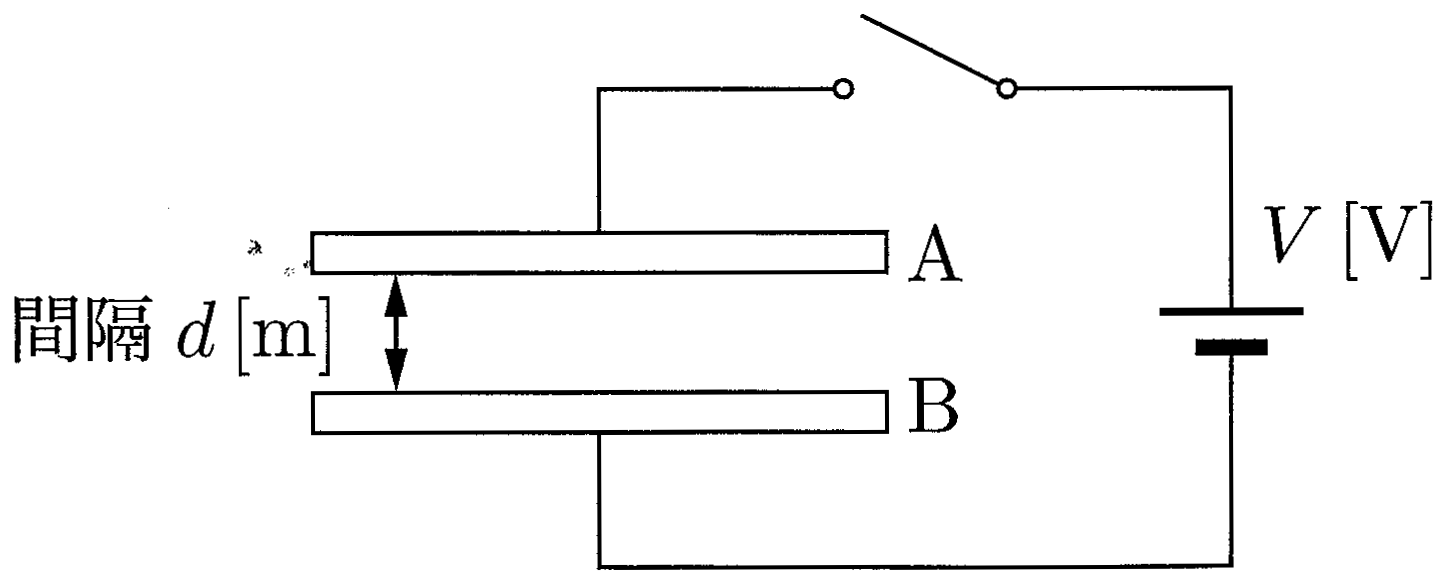
\includegraphics[keepaspectratio,width=62mm]{fig/n25_ex6_zu.png}
\end{zuright}
\begin{komon}
\ko{2} (1)の状態から，電池を接続したまま極板間隔を$2d\U{m}$にした．このときのコンデンサーの電気容量，蓄えられる電荷，静電エネルギー，およびコンデンサー間に作られる電場の大きさを求めよ．
\ko{3} (1)の状態から，電池を外してから極板間隔を$2d\U{m}$にした．このとき蓄えられる電荷，静電エネルギー，両極板間の電位差，およびコンデンサー間に作られる電場の大きさを求めよ．
\end{komon}
\end{reidai}

\begin{sisinE}
極板間隔を変える問題では，{\gtfamily 操作の前後でどの量が変化せず，どの量が変化するのか}を最初に押さえることが何より大切である．

電池をつないだままなら{\gtfamily 極板間の電圧$V$が一定}，電池を外してあるなら{\gtfamily 極板上の電荷$Q$が一定}である．
それ以外の量は，はっきり「変わらない」と読み取れない限りすべて変化しうると考えて，$C=\varepsilon_0\dfrac{S}{d}$で新しい電気容量を出したうえで$Q=CV$・$U$・$E=\dfrac{V}{d}$を一つずつ求め直すこと．
\end{sisinE}

\Key{$C=\varepsilon_0\dfrac{S}{d}\U{F}$\quad $Q=CV\U{C}$\quad $U=\dfrac{Q^2}{2C}=\dfrac{1}{2}QV=\dfrac{1}{2}CV^2\U{J}$}

\begin{kaitou}
\begin{komon}
\ko{1} コンデンサーには電池の電圧$V$がかかるので，
       \[Q=CV\U{C}\Ans\]
       \[U=\frac{1}{2}CV^2\U{J}\Ans\]
       極板間は一様電場だから，$V=Ed$より
       \[E=\frac{V}{d}\U{V/m}\Ans\]
\ko{2} 極板間隔が$2d$になったので，$C=\varepsilon_0\dfrac{S}{d}$より電気容量は
       \[C^\prime=\varepsilon_0\frac{S}{2d}=\frac{1}{2}C\U{F}\Ans\]
       電池を接続したままなので極板間の電圧は$V$のまま変化しない．よって
       \[Q^\prime=C^\prime V=\frac{1}{2}CV\U{C}\Ans\]
       \[U^\prime=\frac{1}{2}C^\prime V^2=\frac{1}{4}CV^2\U{J}\Ans\]
       \[E^\prime=\frac{V}{2d}\U{V/m}\Ans\]
\ko{3} 電池を外してから極板間隔を変えたので，{\gtfamily 極板上の電荷が変化しない}．電気容量は(2)と同じく$C^{\prime\prime}=\dfrac{1}{2}C\U{F}$であるから，
       \[Q^{\prime\prime}=Q=CV\U{C}\Ans\]
       \Ana{U^{\prime\prime}=\frac{(Q^{\prime\prime})^2}{2C^{\prime\prime}}=\frac{(CV)^2}{2\cdot\frac{1}{2}C}=CV^2\U{J}\Ans}
       また，極板間の電位差は
       \[V^{\prime\prime}=\frac{Q^{\prime\prime}}{C^{\prime\prime}}=2V\U{V}\Ans\]
       であり，極板間隔が$2d$であるから
       \[E^{\prime\prime}=\frac{V^{\prime\prime}}{2d}=\frac{V}{d}\U{V/m}\Ans\]
       \begin{chuu}
       (3)で$E^{\prime\prime}=E$となった．$E=\dfrac{Q}{\varepsilon_0S}$と書き直せば分かるように，{\gtfamily 極板上の電荷が変わらなければ極板間の電場は極板間隔によらない}．極板間の電場を作るのは極板上の電荷から出る電気力線であり，電荷が同じなら電気力線の様子は間隔を変えても変わらないからである．
       \end{chuu}
\end{komon}
\end{kaitou}
\end{reidaiunit}

\subsection{誘電体}

\begin{zuright}{40mm}
\hspace{1zw}コンデンサーの電気容量を増やすためには極板面積を大きく，極板間隔を小さくすればよいが，そのほかに，コンデンサーの極板間に絶縁体（{\gtfamily 誘電体}ともよぶ）を入れることによっても電気容量を増やすことができる．
\par
\hspace{1zw}誘電体は，金属などと異なり，電子がその原子核に比較的強く束縛されている．
通常の，外部電場の存在しない状態では電子の重心位置と核の位置とは一致しているが，これに外部から電場をかけるとその電場により原子核と電子の重心がずれ，その結果，元の状態と比較して微小電荷が生じた状態となる．
この現象を{\gtfamily 誘電分極}という．
\zusep

\includegraphics[keepaspectratio,width=40mm]{text2_p38_fig1.png}
\end{zuright}

\begin{zuright}{40mm}
\hspace{1zw}このため，誘電体を挟み込んだコンデンサーに電圧$V\U{V}$の電池を接続した場合，誘電分極により生じた電荷によって極板上の電荷が見かけ上少なくなる．
これを補うために，より多くの電荷を蓄えることが可能となる．
極板間が真空の場合の電気容量を$C_0\U{F}$，極板間を誘電体で満たした場合の電気容量を$C^\prime\U{F}$とするとき，その容量比を{\gtfamily 比誘電率}とよぶ．
\[\varepsilon_{\mathrm{r}}=\frac{C^\prime}{C_0}\]
\zusep

\includegraphics[keepaspectratio,width=40mm]{text2_p38_fig2.png}
\end{zuright}

ここで，比誘電率$\varepsilon_{\mathrm{r}}$は必ず$1$より大きな値となる．
比誘電率が$\varepsilon_{\mathrm{r}}$のコンデンサーの電気容量は
\[C^\prime=\varepsilon_{\mathrm{r}}\varepsilon_0\frac{S}{d}\U{F}\]
と書けるので，この$\varepsilon=\varepsilon_{\mathrm{r}}\cdot\varepsilon_0\U{C^2/N\cdot m^2}$をその誘電体の{\gtfamily 誘電率}とよぶ．

% 加筆（2026-09-24）：練習［50］の指針が「誘電体は極板間に引き込まれる方向に力を受ける」を
%   前提にしているが，原本の本文にはどこにも書かれていなかった．
なお，誘電体を入れた方が同じ電荷に対する静電エネルギーが小さくなるので（練習［50］），自然界はより安定な状態になろうとするという原則から，{\gtfamily 誘電体は極板間に引き込まれる向きに力を受ける}．
逆に誘電体を引きずり出すには，この力に逆らって外力を加えなければならない．

\bsNeed{36mm}
\begin{matome}{誘電体の挿入}
 \hspace{3mm} 比誘電率$\varepsilon_{\mathrm{r}}$の誘電体の誘電率は
 \[\varepsilon=\varepsilon_{\mathrm{r}}\cdot\varepsilon_0\U{C^2/N\cdot m^2}\]
 \hspace{3mm} 誘電率$\varepsilon\U{C^2/N\cdot m^2}$のコンデンサーの電気容量は
 \AnaBD{C^\prime=\varepsilon\frac{S}{d}=\varepsilon_{\mathrm{r}}\varepsilon_0\frac{S}{d}\U{F}}
\end{matome}

%%%%%%%%%%  例題7（25.3 の直後。原本の【例題9】）  %%%%%%%%%%%%%%%%%%%%
\bsNeed{86mm}
\begin{reidaiunit}
\begin{reidai}{誘電体}
\hspace{1zw}極板間隔$d\U{m}$，電気容量$C_0\U{F}$の平行平板コンデンサーをスイッチ$\mathrm{K}$を経て，起電力$V\U{V}$の電池につないだ．以下の設問に答えよ．
\begin{komon}
\ko{1} スイッチ$\mathrm{K}$を閉じるとき，極板に溜まる電荷$Q_0\U{C}$および極板間の電場の強さ$E_0\U{N/C}$を求めよ．
\ko{2} $\mathrm{K}$を開き，比誘電率$\varepsilon_{\mathrm{r}}$，厚さ$d\U{m}$の雲母板を極板間に挿入して満たした．極板間の電場の強さ$E^\prime\U{N/C}$，極板間電圧$V^\prime\U{V}$，および電気容量$C^\prime\U{F}$を求めよ．
\ko{3} 続いて$\mathrm{K}$を閉じた．$\mathrm{K}$を通して$\mathrm{G}\rightarrow\mathrm{H}$の向きに流れる電気量はどれだけか．$\mathrm{G}\rightarrow\mathrm{H}$の向きに流れる電気量を正として答えよ．また，このときの極板間の電場の強さ$E^{\prime\prime}\U{N/C}$を求めよ．
\end{komon}
\begin{center}
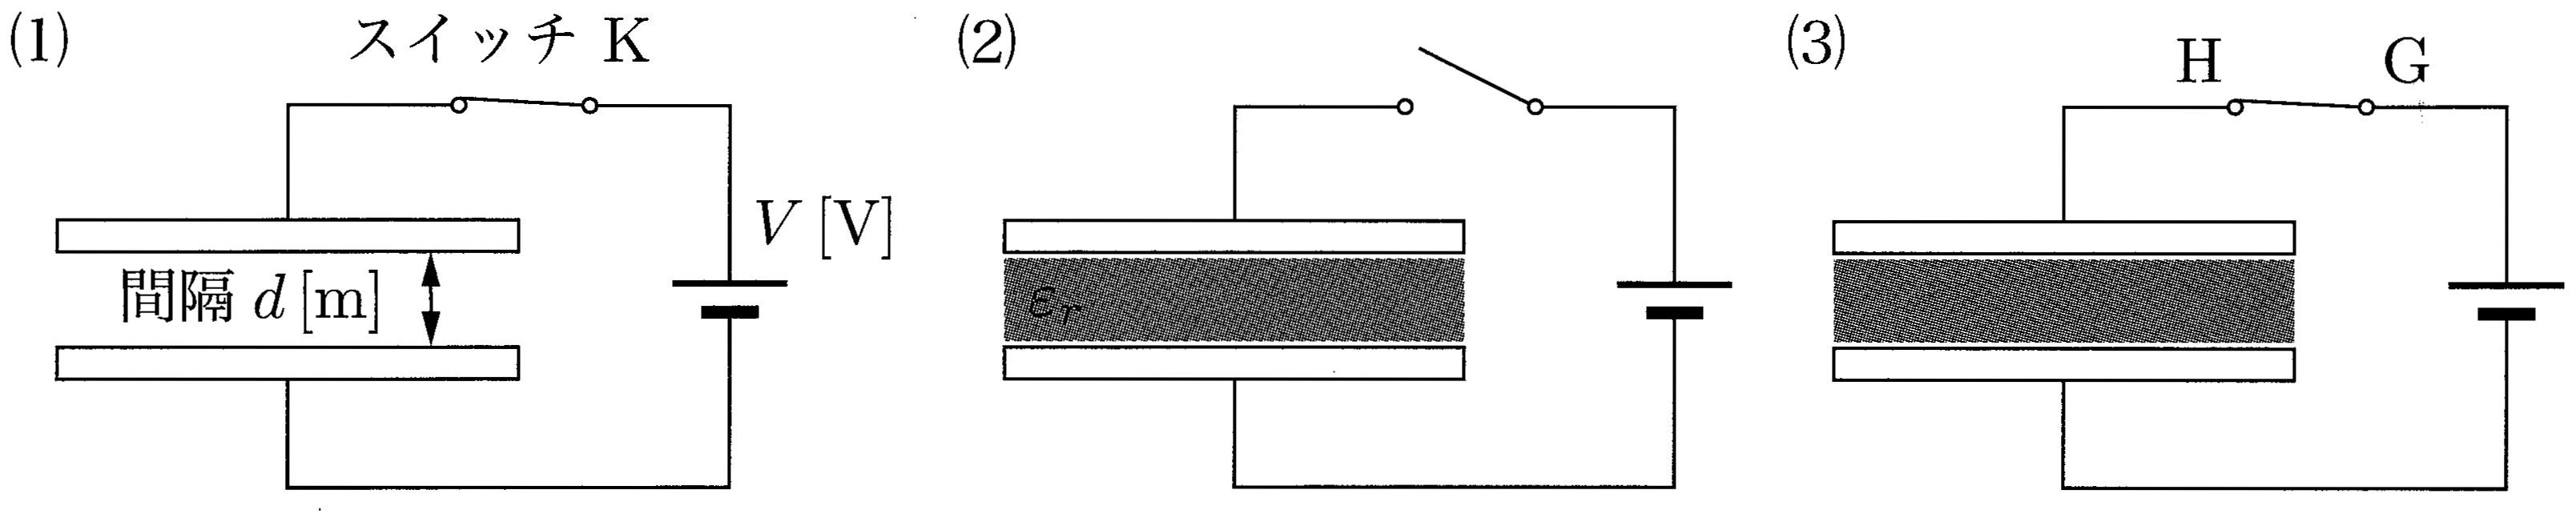
\includegraphics[keepaspectratio,width=150mm]{fig/n25_ex7_zu.png}
\end{center}
\end{reidai}

\begin{sisinE}
例題6と同じく，{\gtfamily どの量が変わらないか}から出発する．$\mathrm{K}$が開いていれば極板上の電荷が，閉じていれば極板間の電圧が保存される．

誘電体を差し込んだ場合の電気容量の変化は，そのつど$C=\varepsilon\dfrac{S}{d}$に戻って計算し，それを元の電気容量$C_0$で表すようにするとよい．
(3)でスイッチを通過する電気量は，{\gtfamily 操作の前後で極板上の電荷がどれだけ増えたか}を計算し，その増加分がどちら向きに流れ込んだのかを考える．
\end{sisinE}

\Key{$C=\varepsilon_0\dfrac{S}{d}\U{F}$\quad $Q=CV\U{C}$\quad $\varepsilon=\varepsilon_{\mathrm{r}}\cdot\varepsilon_0$\quad $C^\prime=\varepsilon\dfrac{S}{d}\U{F}$}

\begin{kaitou}
\begin{komon}
\ko{1} $\mathrm{K}$を閉じるとコンデンサーには電圧$V$がかかるので，
       \[Q_0=C_0V\U{C}\Ans\]
       \[E_0=\frac{V}{d}\U{N/C}\Ans\]
\ko{2} $\mathrm{K}$を開いたので極板上の電荷は$Q_0=C_0V$のまま保存する．雲母板で満たした後の電気容量は，$C_0=\varepsilon_0\dfrac{S}{d}$であることから
       \[C^\prime=\varepsilon_{\mathrm{r}}\varepsilon_0\frac{S}{d}=\varepsilon_{\mathrm{r}}C_0\U{F}\Ans\]
       よって極板間電圧は
       \[V^\prime=\frac{Q_0}{C^\prime}=\frac{C_0V}{\varepsilon_{\mathrm{r}}C_0}=\frac{V}{\varepsilon_{\mathrm{r}}}\U{V}\Ans\]
       であり，極板間隔は$d$のままだから
       \[E^\prime=\frac{V^\prime}{d}=\frac{V}{\varepsilon_{\mathrm{r}}d}\U{N/C}\Ans\]
\ko{3} 再び$\mathrm{K}$を閉じると極板間には電池の電圧$V$がかかるので，このとき極板に蓄えられる電荷は
       \[Q^{\prime\prime}=C^\prime V=\varepsilon_{\mathrm{r}}C_0V\U{C}\]
       である．上側極板の電荷は$+C_0V$から$+\varepsilon_{\mathrm{r}}C_0V$へと増加しており，その増加分は電池側から$\mathrm{K}$を通って上側極板へ流れ込んだと考えられる．よって$\mathrm{G}\rightarrow\mathrm{H}$の向きに流れた電気量は
       \Ana{Q^{\prime\prime}-Q_0=(\varepsilon_{\mathrm{r}}-1)C_0V\U{C}\Ans}
       また，極板間電圧は$V$に戻り極板間隔は$d$のままだから
       \[E^{\prime\prime}=\frac{V}{d}\U{N/C}\Ans\]
       \begin{chuu}
       $\varepsilon_{\mathrm{r}}>1$なので答えは正である．すなわち電気量は確かに$\mathrm{G}\rightarrow\mathrm{H}$の向きに流れた．
       \end{chuu}
\end{komon}
\end{kaitou}
\end{reidaiunit}

\subsection{キルヒホッフの第二法則と電荷保存の法則}

前節まで学んだコンデンサーと電池およびスイッチを導線でつなぐと様々な回路を作ることができるが，スイッチを開閉したときにコンデンサーにどのように電荷が蓄えられるかを考えるためには，{\gtfamily 電荷保存の法則}と{\gtfamily キルヒホッフの第二法則}とを組み合わせて考えていけばよい．

\begin{zuright}{54mm}
\hspace{1zw}電気回路において，導線中（導体中）の電位は必ず一定であるから，（急激な電荷の移動がなければ）{\gtfamily 導線でつながっているところは必ず等電位になっている}．
そして，{\gtfamily 電池や回路中の素子（コンデンサーや抵抗など）で電位が高くなったり低くなったりする}．
このとき，{\gtfamily 回路上の任意の閉ループをひと回りした場合には，必ず同じ電位に戻ってくる}．
これを{\gtfamily キルヒホッフの第二法則}という．
\zusep

\includegraphics[keepaspectratio,width=54mm]{text2_p40_fig1.png}
\end{zuright}

% 加筆（2026-09-24）：原本 p40 にある「立式の形」が旧 physics_ch32.tex では落ちていた．
立式するときは，起電力の総和を左辺に，素子にかかっている電圧（電圧降下）の総和を右辺にまとめて等号で結ぶ．
\[\underbrace{\sum E}_{\text{起電力の総和}}=\underbrace{\sum V}_{\text{電圧降下の総和}}\]
回路のキルヒホッフの法則は，右図のように{\gtfamily 導線部分を平坦な道，素子を坂道に例えて}捉えると分かりやすい．

コンデンサーを組み合わせて作られた回路で，各コンデンサーに蓄えられる電荷を求めるためには，各コンデンサーに蓄えられる電荷を文字で置き，回路のキルヒホッフ第二法則を立てればよい．

\bsNeed{22mm}
\begin{matome}{キルヒホッフの第二法則}
 \hspace{3mm} 回路上の任意の閉ループをひと回りした場合には，必ず\,\AnaB{同じ電位}\,に戻ってくる．
 \[\text{（起電力の総和）}=\text{（電圧降下の総和）}\]
\end{matome}

\begin{zuright}{46mm}
\hspace{1zw}また，電荷は電子の過不足により生じるものであるから，例えば右図のように{\gtfamily 他の回路から離れているような部分回路ではその内部で電子が移動するのみであるから，その全電気量は不変である}．
これを{\gtfamily 電荷保存の法則}という．
\par
\hspace{1zw}コンデンサー回路を考えていくときは，このような，{\gtfamily 他の回路から浮いている部分（孤立した部分）を発見し}，その部分に電荷保存の法則を考えていくことが大切である．
\zusep

\includegraphics[keepaspectratio,width=46mm]{text2_p40_fig2.png}
\end{zuright}

コンデンサーでは，向かい合う極板には必ず正負逆，大きさが同じ電荷が蓄えられるが，{\gtfamily 正の電荷が蓄えられている側がより高電位}である．

% 加筆（2026-09-24）：接地（アース）の意味が原本の本文になく，練習［54］［59］の
%   電荷保存の議論（接地された部分には電荷保存を使わない）が前提にしている．
%   原本では［59］の指針で初めて出てくる状態だった．
第24回で見たように，回路の一点を大地につなぐことを{\gtfamily 接地}（アース）といい，接地した点の電位を$0\U{V}$とする．
アースは正負の電荷が自由に出入りできるので，コンデンサー回路では{\gtfamily 接地された部分は「他から浮いている部分」ではなくなる}．
電荷保存の法則を使う範囲を探すときは，接地された導線を含む部分を選んではならない．

\bsNeed{26mm}
\begin{matome}{電荷保存の法則}
 \hspace{3mm} 他の部分から浮いている（孤立した）回路部分の全電気量は保存される．\\[1mm]
 \hspace{3mm} ただし\,\AnaB{接地}\,された部分は，大地との間で電荷が出入りできるので対象にしない．
\end{matome}

\subsection{コンデンサーの並列接続と直列接続}

コンデンサーを2つ組み合わせるつなぎ方には，両端どうしをそろえてつなぐ{\gtfamily 並列接続}と，数珠つなぎにする{\gtfamily 直列接続}とがある．
どちらの場合も，25.4の2つの法則だけで各コンデンサーの帯電量が求まる．
並列接続を例題8で，直列接続を例題9で，同じ手順で解いて比べてみよう．

%%%%%%%%%%  例題8（25.5。原本の【例題10】）  %%%%%%%%%%%%%%%%%%%%
\bsNeed{74mm}
\begin{reidaiunit}
\begin{reidai}{コンデンサーの並列接続}
\begin{zuright}{44mm}
\hspace{1zw}右図のように，電気容量$C_1\U{F}$，$C_2\U{F}$のコンデンサーを並列につなぎ，スイッチ$\mathrm{S}$を経て起電力$V\U{V}$の電池につないだ．最初，スイッチ$\mathrm{S}$は開いており，各コンデンサーに電荷は蓄えられていなかった．以下の設問に答えよ．
\begin{komon}
\ko{1} スイッチ$\mathrm{S}$を閉じてから十分時間がたったのちの，各コンデンサーに蓄えられている電気量を求めよ．
\ko{2} スイッチ$\mathrm{S}$を閉じてから(1)の状態に至るまでに導線で失われたエネルギーを求めよ．
\end{komon}
\zusep
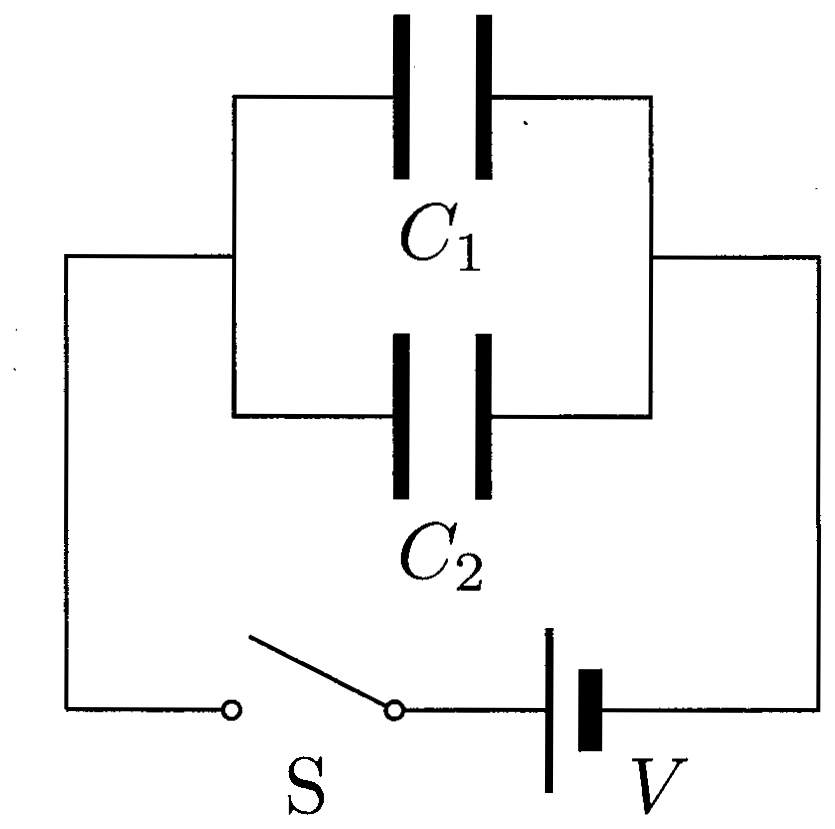
\includegraphics[keepaspectratio,width=44mm]{fig/n25_ex8_zu.png}
\end{zuright}
\end{reidai}

\begin{sisinE}
並列につながれた2つのコンデンサーは，どちらも両端が電池の両極と導線だけで結ばれている．
導線でつながっているところは等電位だから，{\gtfamily どちらのコンデンサーにも同じ電圧$V$がかかる}．

(2)は25.2で述べた「電池のした仕事」と「蓄えられた静電エネルギー」の差である．差はすべて導線のわずかな抵抗から熱として失われる．
\end{sisinE}

\Key{$Q=CV\U{C}$\quad 回路上の任意の閉ループをひと回りした場合には，必ず同じ電位に戻ってくる}

\begin{kaitou}
\begin{komon}
\ko{1} $\mathrm{C}_1$，$\mathrm{C}_2$を含む閉ループのそれぞれにキルヒホッフの第二法則を用いると，どちらにかかる電圧も$V$である．よって
       \[Q_1=C_1V\U{C}\Ans\]
       \[Q_2=C_2V\U{C}\Ans\]
\ko{2} 電池を負極側から正極側へ通過した電気量は$Q_1+Q_2=(C_1+C_2)V\U{C}$であるから，電池のした仕事は
       \[W_{\mathrm{E}}=(Q_1+Q_2)V=(C_1+C_2)V^2\U{J}\]
       である．一方，2つのコンデンサーに蓄えられた静電エネルギーの和は
       \[U=\frac{1}{2}C_1V^2+\frac{1}{2}C_2V^2=\frac{1}{2}(C_1+C_2)V^2\U{J}\]
       である．よって導線で失われたエネルギーは
       \Ana{W_{\mathrm{E}}-U=\frac{1}{2}(C_1+C_2)V^2\U{J}\Ans}
       \begin{chuu}
       電池がした仕事のうち，{\gtfamily ちょうど半分}しかコンデンサーに蓄えられない．これは$C_1$，$C_2$の値によらない．
       \end{chuu}
\end{komon}
\end{kaitou}
\end{reidaiunit}

%%%%%%%%%%  例題9（25.5。原本の【例題11】）  %%%%%%%%%%%%%%%%%%%%
\bsNeed{72mm}
\begin{reidaiunit}
\begin{reidai}{コンデンサーの直列接続}
\begin{zuright}{44mm}
\hspace{1zw}右図のように，電気容量$C_1\U{F}$，$C_2\U{F}$のコンデンサーを直列につなぎ，スイッチ$\mathrm{S}$を経て起電力$V\U{V}$の電池につないだ．最初，スイッチ$\mathrm{S}$は開いており，各コンデンサーに電荷は蓄えられていなかった．以下の設問に答えよ．
\begin{komon}
\ko{1} スイッチ$\mathrm{S}$を閉じてから十分時間がたったのちの，各コンデンサーの左側極板に蓄えられている電気量を$Q_1\U{C}$，$Q_2\U{C}$とおく．このとき，$Q_1$，$Q_2$の間に成り立つ関係式を2つ示せ．
\ko{2} $Q_1$，$Q_2$を求めよ．
\end{komon}
\zusep
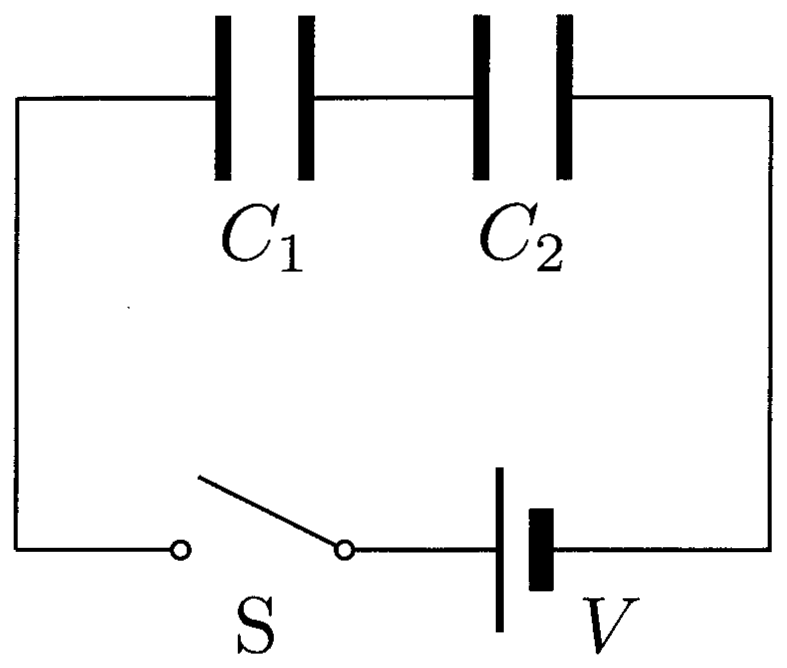
\includegraphics[keepaspectratio,width=44mm]{fig/n25_ex9_zu.png}
\end{zuright}
\end{reidai}

\begin{sisinE}
$\mathrm{C}_1$の右側極板と$\mathrm{C}_2$の左側極板は，導線でつながっているだけでほかのどこにもつながっていない．
つまりこの部分は{\gtfamily 他から浮いている}ので，ここに電荷保存の法則が使える．
これが1本目の式である．

2本目は，電池と2つのコンデンサーを通る閉ループについてのキルヒホッフの第二法則である．
\end{sisinE}

\Key{$Q=CV$\quad 閉ループをひと回りすると同じ電位に戻る\quad 浮いている部分の全電気量は保存される}

\begin{kaitou}
\begin{komon}
\ko{1} 左側極板の電荷を$+Q_1$，$+Q_2$とすると，向かい合う極板の電荷はそれぞれ$-Q_1$，$-Q_2$である．
       $\mathrm{C}_1$の右側極板と$\mathrm{C}_2$の左側極板からなる浮いた部分について，もともと電荷が無かったので電荷保存の法則より
       \[-Q_1+Q_2=0\qquad\text{すなわち}\qquad Q_1=Q_2\Ans\]
       また，電池と2つのコンデンサーを通る閉ループにキルヒホッフの第二法則を用いると
       \[V=\frac{Q_1}{C_1}+\frac{Q_2}{C_2}\Ans\]
\ko{2} 上の2式から$Q_2$を消去して
       \Ana{Q_1=Q_2=\frac{C_1C_2}{C_1+C_2}V\U{C}\Ans}
\end{komon}
\end{kaitou}
\end{reidaiunit}

% 加筆（2026-09-24）：原本の本文には合成容量が無く，例題10・例題11 で導いたきり
%   まとめられていなかった（練習［53］の指針は「コンデンサーの合成」に言及している）．
例題8・例題9の結果を，「1個のコンデンサーで置き換えるとしたら容量はいくつか」という形に読み替えておくと便利である．
並列接続では両方に同じ電圧$V$がかかって合計$(C_1+C_2)V$の電荷を蓄えるので，合成容量は$C_1+C_2$である．
直列接続では蓄えられる電荷が$\dfrac{C_1C_2}{C_1+C_2}V$なので，合成容量は$\dfrac{C_1C_2}{C_1+C_2}$，すなわち逆数の和が$\dfrac{1}{C_1}+\dfrac{1}{C_2}$となる．

\bsNeed{44mm}
\begin{matome}{コンデンサーの合成容量}
 \hspace{3mm} 並列接続（両方に同じ電圧がかかる）
 \[C=C_1+C_2\U{F}\]
 \hspace{3mm} 直列接続（両方に同じ電荷が蓄えられる）
 \AnaBD{\frac{1}{C}=\frac{1}{C_1}+\frac{1}{C_2}\qquad\text{すなわち}\qquad C=\frac{C_1C_2}{C_1+C_2}\U{F}}
\end{matome}

\subsection{コンデンサー回路の解き方}

キルヒホッフ第二法則と電荷保存の法則を組み合わせると，様々なコンデンサー回路の電荷分布の変化を計算することができる．
その方針をここで再度まとめておく．

\bsNeed{40mm}
\begin{matome}{コンデンサー回路の解き方}
\begin{description}
\item[\MARU{1}] 各コンデンサーの帯電量を文字$+q\U{C}$，$-q\U{C}$などでおく．
\item[\MARU{2}] 回路の浮いている部分について，\AnaB{電荷保存}\,の法則を適用する．
\item[\MARU{3}] 帯電量$+q\U{C}$側の極板の方が$\dfrac{q}{C}\U{V}$だけ電位が高いことを利用して，\AnaB{キルヒホッフ}\,の第二法則を立てる．
\end{description}
\end{matome}
% 原本 p41 のまとめ枠は③が「帯電量 $-q$ 側の極板の方が…電位が高い」と誤植されている
% （同じ枠が p42 の例題12の KEY では $+q$ になっていて，そちらが正しい）．$+q$ を採用した．

なお，スイッチを切り替える問題では，{\gtfamily 切り替えの前と後の回路図を必ず両方書き出し，それぞれに各極板の帯電量を書き込む}こと．
そのうえで「操作の前後で他の部分と接続していない部分」を探せば，そこが電荷保存の法則を使える場所である．

また，回路に{\gtfamily 検流計}（通過した電気量を測る装置）が入っている場合，定常状態では電荷が移動していないので検流計に電圧はかからない．
キルヒホッフの第二法則を立てる際には{\gtfamily ただの導線と同じ}に扱えばよい．

%%%%%%%%%%  例題10（25.6 の直後。原本の【例題12】）  %%%%%%%%%%%%%%%%%%%%
\bsNeed{62mm}
\begin{reidaiunit}
\begin{reidai}{コンデンサー回路}
\begin{zuright}{52mm}
\hspace{1zw}起電力$V\U{V}$の電池$\mathrm{E}_1$，$\mathrm{E}_2$および電気容量が$C_1\U{F}$，$C_2\U{F}$のコンデンサー$\mathrm{C}_1$，$\mathrm{C}_2$，スイッチ$\mathrm{S}_1$，$\mathrm{S}_2$，$\mathrm{S}_3$を用いて右図のような回路を作る．回路の左下を接地してこの点の電位を$0\U{V}$とする．今，スイッチがすべて開いた状態で，2つのコンデンサーのいずれにも電荷は蓄えられていない．以下の設問に答えよ．
\zusep
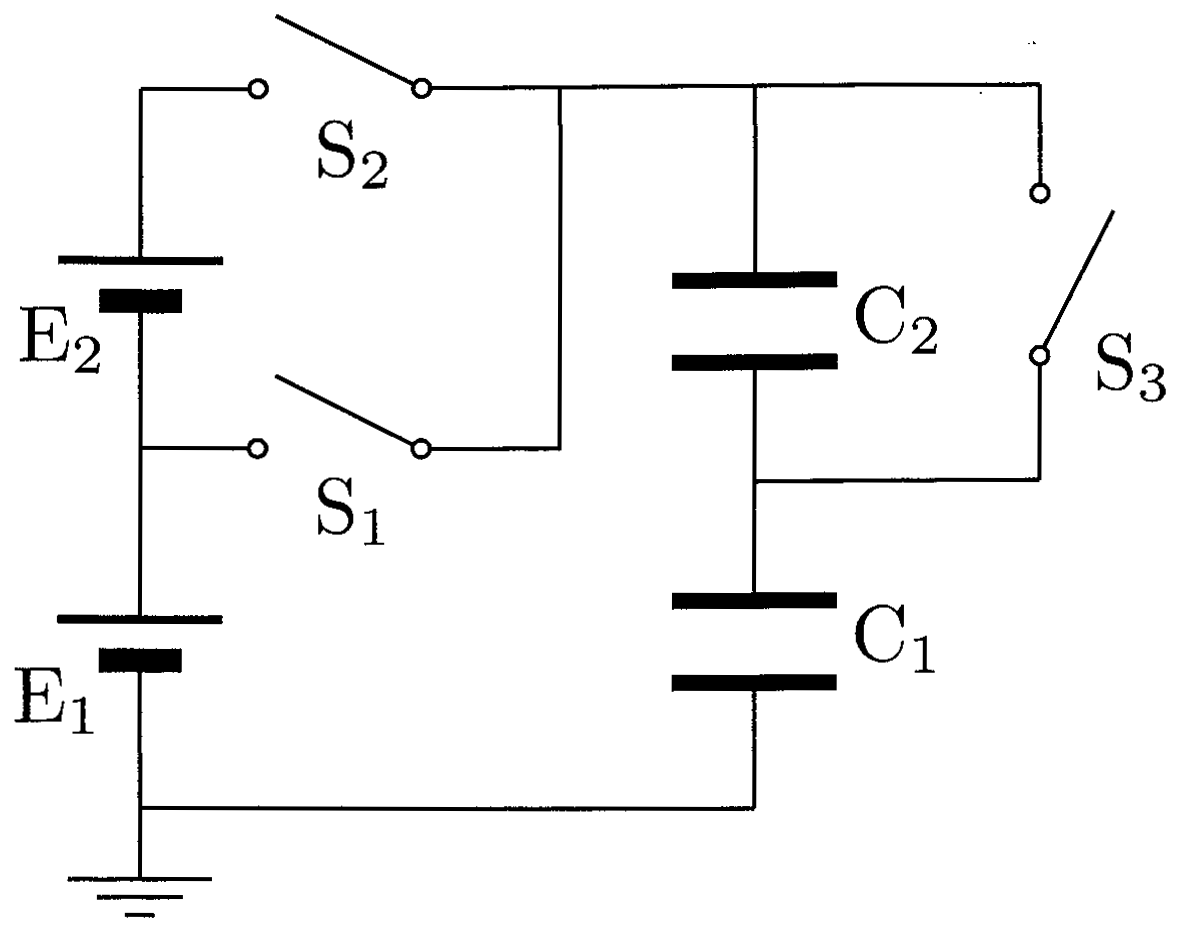
\includegraphics[keepaspectratio,width=52mm]{fig/n25_ex10_zu.png}
\end{zuright}
\begin{komon}
\ko{1} スイッチ$\mathrm{S}_2$，$\mathrm{S}_3$のみを閉じる．このとき，コンデンサー$\mathrm{C}_1$の上側極板に蓄えられる電荷$Q_0\U{C}$を求めよ．
\ko{2} 次に$\mathrm{S}_2$，$\mathrm{S}_3$を開き，その後でスイッチ$\mathrm{S}_1$を閉じた．このとき，コンデンサー$\mathrm{C}_1$の上側極板に蓄えられる電荷$Q_1\U{C}$およびコンデンサー$\mathrm{C}_2$の上側極板の電荷$Q_2\U{C}$を求めよ．
\ko{3} (2)のとき，コンデンサー$\mathrm{C}_1$と$\mathrm{C}_2$とを結んでいる導線の電位はいくらか．
\end{komon}
\end{reidai}

\begin{sisinE}
まず，接地点を$0\U{V}$として{\gtfamily 各部分の電位を書き込む}ところから始める．
$\mathrm{E}_1$，$\mathrm{E}_2$はどちらも起電力$V$なので，$\mathrm{E}_1$と$\mathrm{E}_2$の間の点は$V\U{V}$，$\mathrm{E}_2$の上端は$2V\U{V}$である．
$\mathrm{S}_1$を閉じれば上側の導線が$V\U{V}$に，$\mathrm{S}_2$を閉じれば$2V\U{V}$になる．

$\mathrm{S}_3$は$\mathrm{C}_2$の両端を結ぶスイッチなので，{\gtfamily $\mathrm{S}_3$を閉じると$\mathrm{C}_2$は短絡されて電圧が$0$になる}．
(2)で$\mathrm{S}_3$を開くと，$\mathrm{C}_2$の下側極板と$\mathrm{C}_1$の上側極板とをつなぐ導線が他とつながらなくなるので，ここに電荷保存の法則が使える．
\end{sisinE}

\Key{接地点を$0\U{V}$として各部の電位を書き込む\quad 浮いている部分に電荷保存\quad 閉ループにキルヒホッフ第二法則}

\begin{kaitou}
\begin{komon}
\ko{1} $\mathrm{S}_2$を閉じたので上側の導線の電位は$2V\U{V}$である．さらに$\mathrm{S}_3$が閉じているので$\mathrm{C}_2$の両端は短絡されており，$\mathrm{C}_1$の上側極板の電位も$2V\U{V}$である．$\mathrm{C}_1$の下側極板は接地されていて$0\U{V}$だから，$\mathrm{C}_1$にかかる電圧は$2V\U{V}$である．よって
       \[Q_0=C_1\cdot 2V=2C_1V\U{C}\Ans\]
\ko{2} $\mathrm{S}_2$，$\mathrm{S}_3$を開いて$\mathrm{S}_1$を閉じたので，上側の導線の電位は$V\U{V}$になる．$\mathrm{C}_1$と$\mathrm{C}_2$を結ぶ導線の電位を$V_{\mathrm{M}}\U{V}$とおく．

       この導線と，そこにつながる$\mathrm{C}_2$の下側極板・$\mathrm{C}_1$の上側極板は，$\mathrm{S}_3$を開いたので{\gtfamily 他の部分から浮いている}．操作前，この部分の電荷は$\mathrm{C}_2$の下側極板が$0$（$\mathrm{C}_2$は短絡されていた），$\mathrm{C}_1$の上側極板が$+Q_0=2C_1V$であったから，電荷保存の法則より
       \[-Q_2+Q_1=2C_1V\]
       また，上側の導線（$V$）→$\mathrm{C}_2$→$\mathrm{C}_1$→接地点（$0$）と回る閉ループにキルヒホッフの第二法則を用いると
       \[V=\frac{Q_2}{C_2}+\frac{Q_1}{C_1}\]
       この2式を解いて，
       \Ana{Q_1=\frac{C_1(2C_1+C_2)}{C_1+C_2}V\U{C}\Ans}
       \[Q_2=-\frac{C_1C_2}{C_1+C_2}V\U{C}\Ans\]
\ko{3} $\mathrm{C}_1$の下側極板が$0\U{V}$であるから，求める電位は
       \[V_{\mathrm{M}}=\frac{Q_1}{C_1}=\frac{2C_1+C_2}{C_1+C_2}V\U{V}\Ans\]
       \begin{chuu}
       $Q_2<0$となったのは，$\mathrm{C}_2$の上側極板が負に帯電しているという意味である．実際$V_{\mathrm{M}}>V$（下側極板の方が高電位）なので，これは正しい．
       仮定した電荷の正負が逆でも，符号をつけたまま答えればよい．
       \end{chuu}
\end{komon}
\end{kaitou}
\end{reidaiunit}

\subsection{複合極板コンデンサー}

今までは極板が2枚の平行平板コンデンサーを扱ってきたが，この極板間に導体を挟んだり，すき間の一部分にのみ誘電体を挿入するなどしたコンデンサーも存在する．
このようなコンデンサーを扱う場合には，以下のようにコンデンサーを書き換えて扱えばよい．

\bsNeed{132mm}
\noindent$\MARU{1}$\hspace{2mm}導体を挟んだコンデンサー：{\gtfamily 導体部を導線だとみなして}2つのコンデンサーに分解する
\begin{center}

\includegraphics[keepaspectratio,width=64mm]{text2_p42_fig1.png}
\end{center}

\noindent$\MARU{2}$\hspace{2mm}誘電体を挟んだコンデンサー：{\gtfamily 誘電体部分を別のコンデンサーだとみなす}
\begin{center}

\includegraphics[keepaspectratio,width=64mm]{text2_p42_fig2.png}
\end{center}

\noindent$\MARU{3}$\hspace{2mm}多極板コンデンサー：{\gtfamily 間に導線を仮想}して複数のコンデンサーに分解する
\begin{center}

\includegraphics[keepaspectratio,width=64mm]{text2_p43_fig1.png}
\end{center}

\noindent$\MARU{4}$\hspace{2mm}並列型に挿入された誘電体：横に分けて{\gtfamily 並列型コンデンサー}だとみなす
\begin{center}

\includegraphics[keepaspectratio,width=64mm]{text2_p43_fig2.png}
\end{center}

複雑なコンデンサーは単純なコンデンサーの合成だとみなして回路を書き換え，25.6のコンデンサー回路の考え方に従って電荷分布を求める．
実際の練習は練習［55］で行う．

\newpage

%%%%%%%%%%%%%%%%%%%%  練習問題  %%%%%%%%%%%%%%%%%%%%
% 第24回の［46］に続く．章単体で組んだときも番号が本体と一致するように明示しておく
\setcounter{qno}{46}

\filbreak
\Rank{A問題}

% A問題の統合（再編案の「A2→1」）：旧㉛[15]（(1)〜(6)）と旧㉜[22]（(1)(2)）を1題にまとめた．
%   設問は1つも失われていない（(7)(8) が旧㉜[22] の(1)(2)）．
\Mon{基本公式の確認}

\hspace{1zw}以下の設問に答えよ．
\begin{komon}
\ko{1} $1.5\U{\mu F}$のコンデンサーに$3.0\times 10^2\U{V}$の電圧をかけると，何$\U{C}$の電荷が蓄えられるか．
\ko{2} $1.5\U{V}$の電圧をかけると，$6.0\times 10^{-6}\U{C}$の電気量を蓄えることのできるコンデンサーの電気容量は何$\U{\mu F}$か．
\ko{3} 電気容量$1.0\U{\mu F}$の平行平板コンデンサーの極板の面積をそのままにして，極板間隔を半分にした．このときの電気容量は何$\U{\mu F}$か．
\ko{4} 極板間距離$2.5\times 10^{-3}\U{m}$の平行平板コンデンサーに$5.0\U{V}$の電圧をかけたとき，極板間にできる電場の強さは何$\U{V/m}$か．
\ko{5} 電気容量$2.0\U{\mu F}$のコンデンサーに，$50\U{V}$の電圧をかけて充電したとき，コンデンサーに蓄えられるエネルギーは何$\U{J}$か．
\ko{6} 電気容量$2.0\U{\mu F}$の平行平板コンデンサーの極板間を，ある誘電体で満たしたところ，その電気容量が$6.0\U{\mu F}$になった．この誘電体の比誘電率はいくらか．
\ko{7} 下図の$\mathrm{C}_1$，$\mathrm{C}_2$はいずれも電気容量が$6.0\U{\mu F}$の，電荷の蓄えられていないコンデンサーである．次のように接続し，$\mathrm{ab}$間にそれぞれ$10\U{V}$の電圧をかけたとき，コンデンサー$\mathrm{C}_1$に蓄えられる電気量は何$\U{\mu C}$か．
\end{komon}
\begin{center}
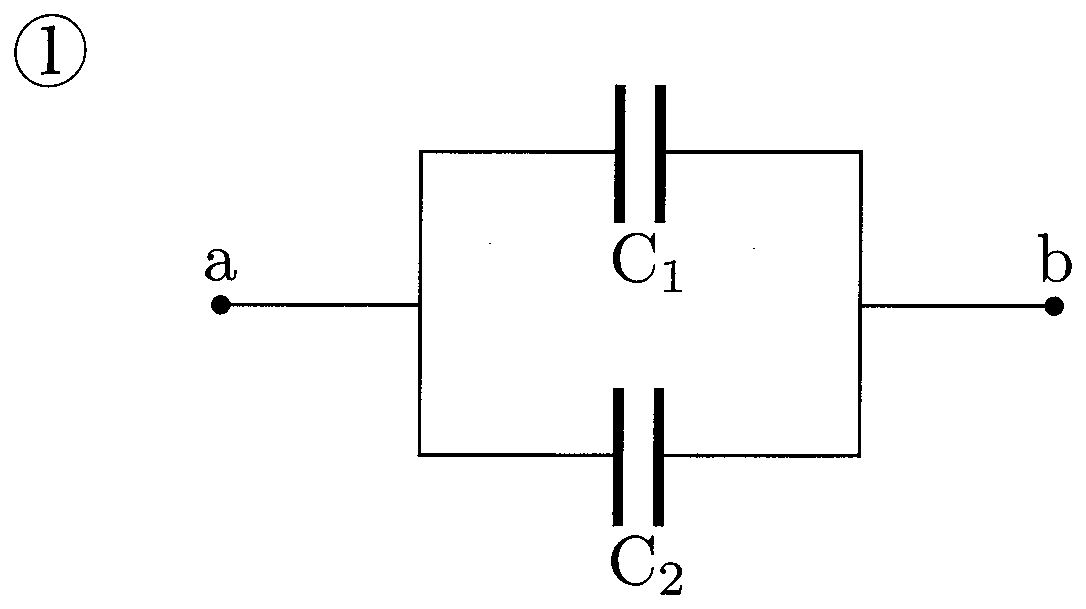
\includegraphics[keepaspectratio,width=72mm]{fig/n25_p47_zu1.png}\hspace{6mm}%
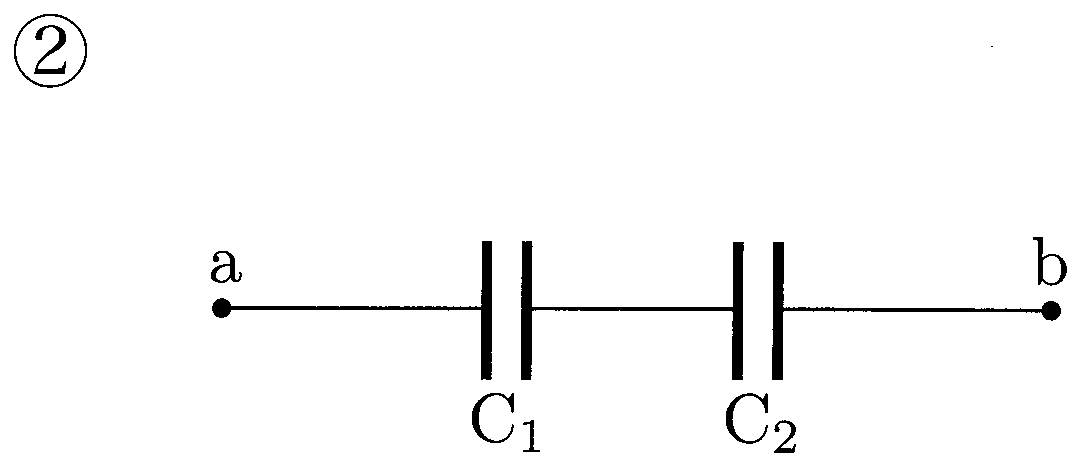
\includegraphics[keepaspectratio,width=68mm]{fig/n25_p47_zu2.png}
\end{center}
\begin{komon}
\ko{8} 極板間が真空であるときの電気容量が$C\U{F}$の平行平板コンデンサーの極板間に，比誘電率が$3$の誘電体を下図のように挿入した．これらのコンデンサーに電圧$V\U{V}$の電池を接続した場合に，コンデンサーの上側極板に蓄えられる電気量を求めよ．
\end{komon}
\begin{center}
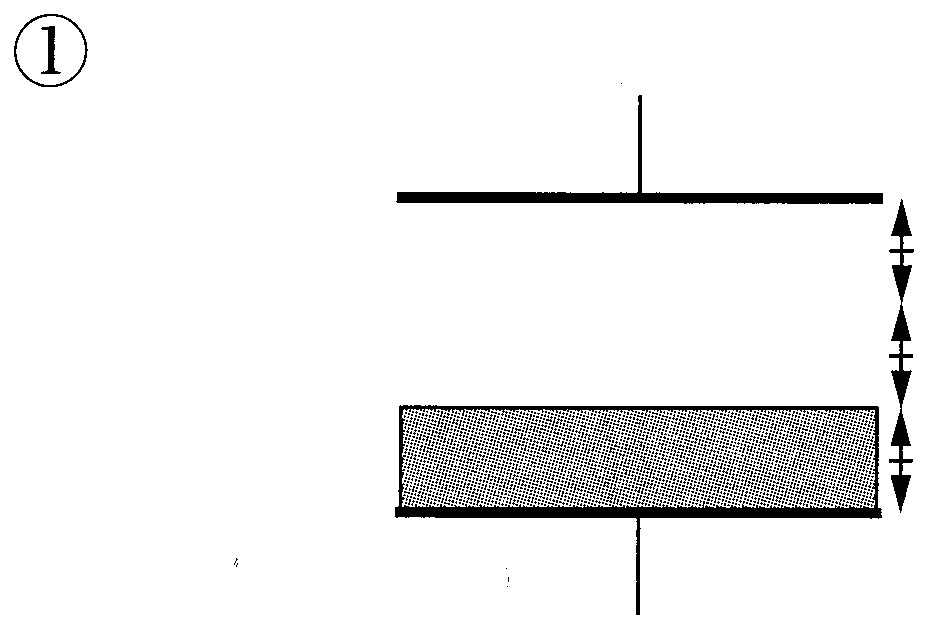
\includegraphics[keepaspectratio,width=60mm]{fig/n25_p47_zu3.png}\hspace{10mm}%
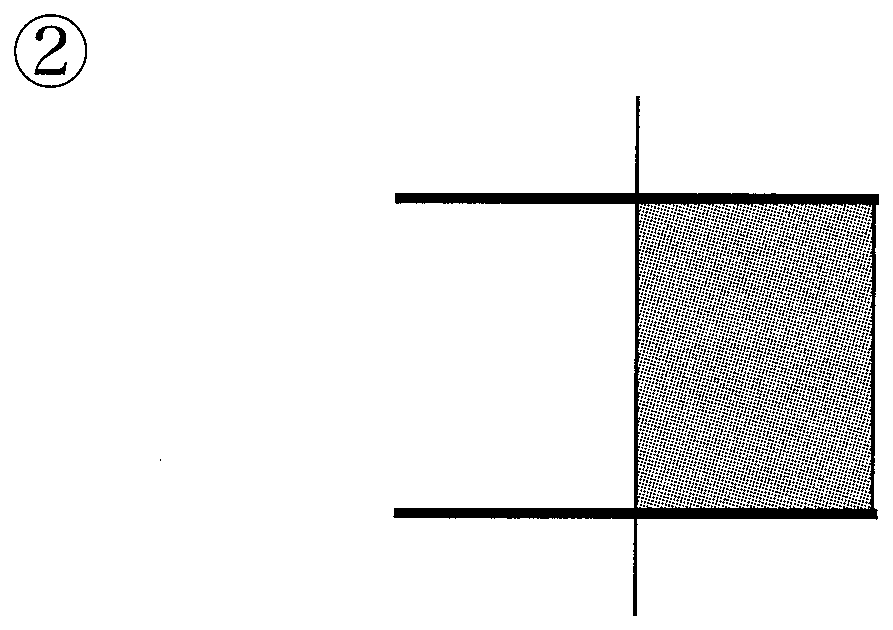
\includegraphics[keepaspectratio,width=58mm]{fig/n25_p47_zu4.png}
\end{center}

\filbreak
\Rank{B問題}

\Mon{平行平板コンデンサーの極板間隔の変化}

\hspace{1zw}断面積$S\U{m^2}$，極板間隔$d\U{m}$，極板間が真空の平行平板コンデンサーに電圧$V\U{V}$の電池を接続した．真空の誘電率を$\varepsilon_0\U{C^2/N\cdot m^2}$として以下の設問に答えよ．
\begin{komon}
\ko{1} このときコンデンサーの電気容量$C\U{F}$，蓄えられる電荷$Q\U{C}$，静電エネルギー$U\U{J}$，および極板間に生じる電場の強さ$E\U{V/m}$を求めよ．
\ko{2} (1)の状態から，電池を接続したまま極板間隔を$kd\U{m}$にした．このときのコンデンサーの電気容量$C^\prime\U{F}$，蓄えられる電気量$Q^\prime\U{C}$，静電エネルギー$U^\prime\U{J}$および極板間に生じる電場の強さ$E^\prime\U{V/m}$を求めよ．
\ko{3} (1)の状態から，電池を外してから極板間隔を$kd\U{m}$にした．このときのコンデンサーの電気容量$C^{\prime\prime}\U{F}$，蓄えられる電気量$Q^{\prime\prime}\U{C}$，静電エネルギー$U^{\prime\prime}\U{J}$および極板間に生じる電場の強さ$E^{\prime\prime}\U{V/m}$を求めよ．
\end{komon}

\Mon[\Sitei]{コンデンサーの極板間の引力}

\hspace{1zw}電気容量$C\U{F}$，間隔$d\U{m}$の平行平板コンデンサーを電圧$V\U{V}$の電池にスイッチ$\mathrm{K}$を通して接続する．コンデンサーに蓄えられるエネルギー$U\U{J}$に関する以下の設問に答えよ．
\begin{komon}
\ko{1} スイッチ$\mathrm{K}$を入れるとき，コンデンサーに蓄えられる電荷$Q_0\U{C}$および静電エネルギー$U_0\U{J}$を求めよ．
\ko{2} 続いて$\mathrm{K}$を開いたのち，極板間隔をゆっくりと3倍に広げた．このとき蓄えられている静電エネルギー$U_1\U{J}$を求めよ．
\ko{3} このエネルギーの変化分は何から得られたか，簡潔に説明せよ．
\ko{4} (2)の極板間隔を広げていく途中において，極板間隔が$x\U{m}$になったときを考える．この状態から，極板間隔を微小距離$dx\U{m}$だけゆっくりと広げた際の静電エネルギーの増加$dU\U{J}$を求めよ．
\ko{5} (4)の微小変化をするとき，ゆっくりと極板間隔を変化させているので，極板間に作用する引力と，加えた外力とが力のつり合いを保ったまま極板が移動する．このことを利用して，極板間に作用する引力$F(x)\U{N}$を求めよ．
\ko{6} (5)で求めた$F(x)\U{N}$を，極板上の電荷$Q_0\U{C}$，真空の誘電率$\varepsilon_0\U{C^2/N\cdot m^2}$，極板面積$S\U{m^2}$を用いて表せ．また同様に，$F(x)\U{N}$を極板上の電荷$Q_0\U{C}$および極板間に作られている電場の強さ$E(x)\U{V/m}$を用いて表せ．
\ko{7} 極板間隔を元に戻し，$\mathrm{K}$を閉じたまま極板間隔を3倍に広げた．このとき蓄えられている静電エネルギー$U_2\U{J}$を求めよ．
\end{komon}
\begin{center}
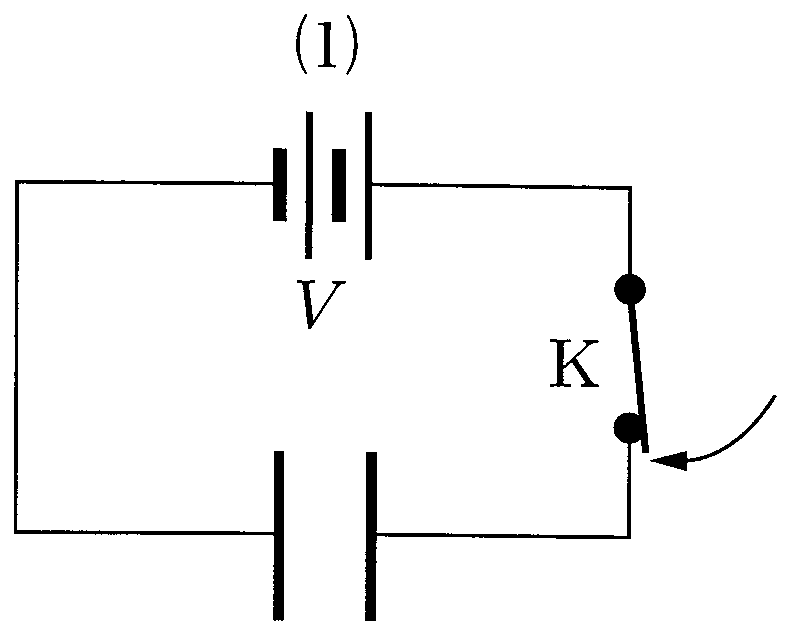
\includegraphics[keepaspectratio,width=48mm]{fig/n25_p49_zu1.png}\hspace{4mm}%
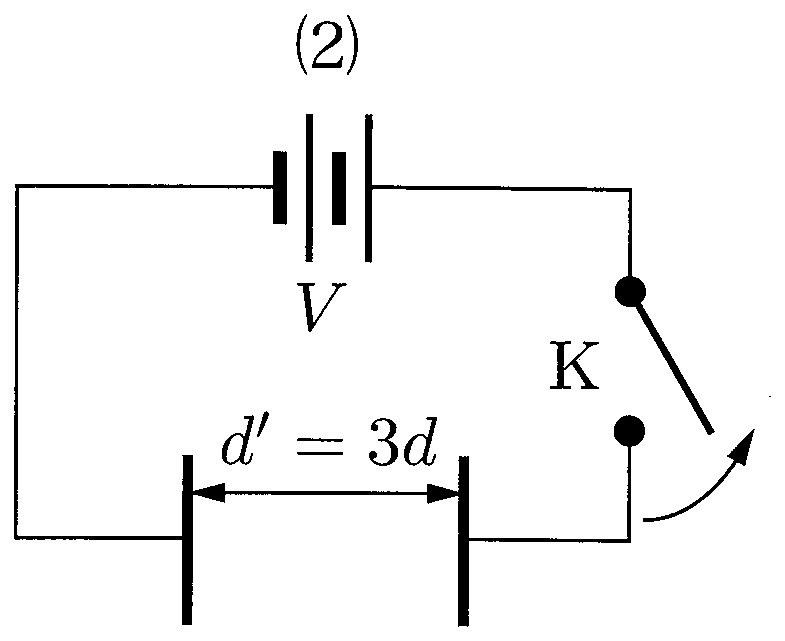
\includegraphics[keepaspectratio,width=48mm]{fig/n25_p49_zu2.png}\hspace{4mm}%
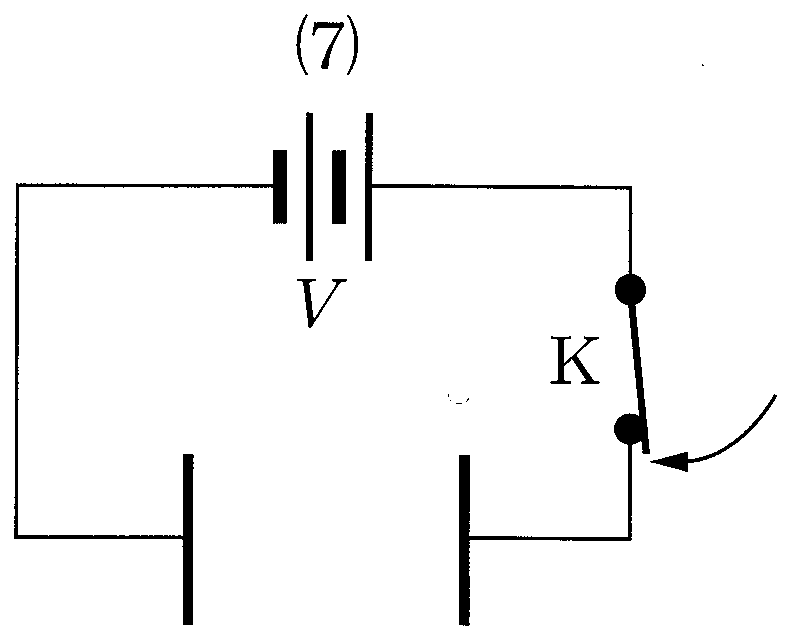
\includegraphics[keepaspectratio,width=48mm]{fig/n25_p49_zu3.png}
\end{center}
\noindent\hspace*{\fill}（左から (1)，(2)，(7) の状態）\hspace*{\fill}

\Mon[\Sitei]{誘電体とコンデンサー}

\begin{zuright}{58mm}
\hspace{1zw}右図のように，比誘電率$\varepsilon_{\mathrm{r}}$の誘電体で満たされた極板面積$S\U{m^2}$，極板間隔$d\U{m}$の平行平板コンデンサーを，スイッチ$\mathrm{K}$を経て起電力$V\U{V}$の電池に接続する．真空の誘電率を$\varepsilon_0\U{C^2/N\cdot m^2}$として以下の問いに答えよ．
\begin{komon}
\ko{1} スイッチ$\mathrm{K}$を閉じて十分な時間を置いたとき，極板に蓄えられる電荷はいくらか．
\end{komon}
\zusep
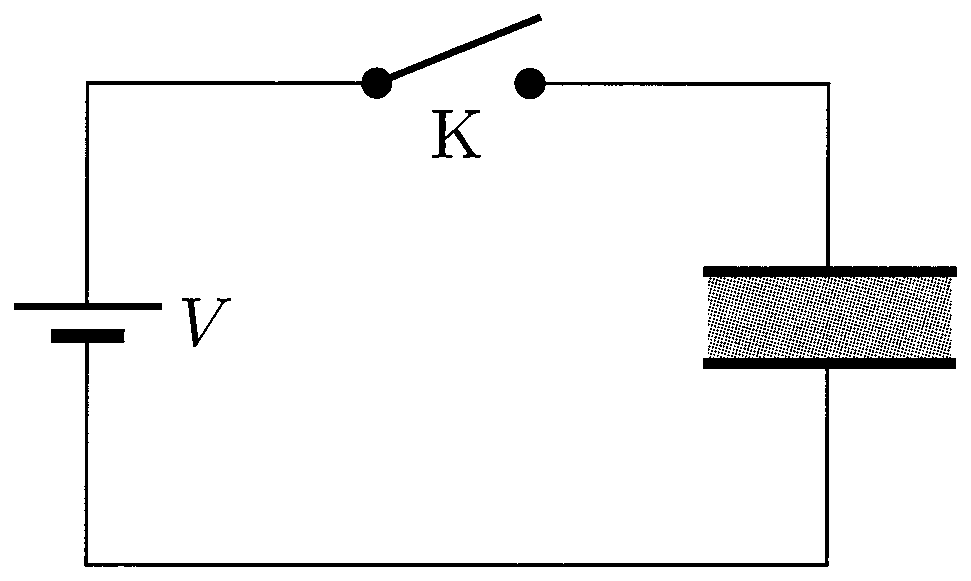
\includegraphics[keepaspectratio,width=58mm]{fig/n25_p50_zu.png}
\end{zuright}
\begin{komon}
\ko{2} $\mathrm{K}$を開き，誘電体を極板間から完全に引き抜いた．このときのコンデンサーの静電エネルギーは(1)の状態に比べてどれだけ変化しているか．もしエネルギーが減少したのならそのエネルギーは何に転化したか，またもし増加しているのであればその増加分は何から与えられたエネルギーか．
\ko{3} (2)の状態から再び$\mathrm{K}$を閉じた．このときスイッチ$\mathrm{K}$を電荷が通過するが，その大きさと通過する向きを求めよ．
\end{komon}

\Mon{並列接続}

\begin{zuright}{62mm}
\hspace{1zw}起電力$V\U{V}$の電池$\mathrm{E}$，スイッチ$\mathrm{S}_1$，$\mathrm{S}_2$，電気容量がそれぞれ$2C$，$C\U{F}$のコンデンサー$\mathrm{C}_1$，$\mathrm{C}_2$が右図のように接続されている．はじめ$\mathrm{C}_1$，$\mathrm{C}_2$には電荷が蓄えられていなかった．各スイッチ操作の後には十分時間を置くものとして，以下の設問に答えよ．
\par
\hspace{1zw}まず$\mathrm{S}_2$を開いたままで$\mathrm{S}_1$を閉じる．
\zusep
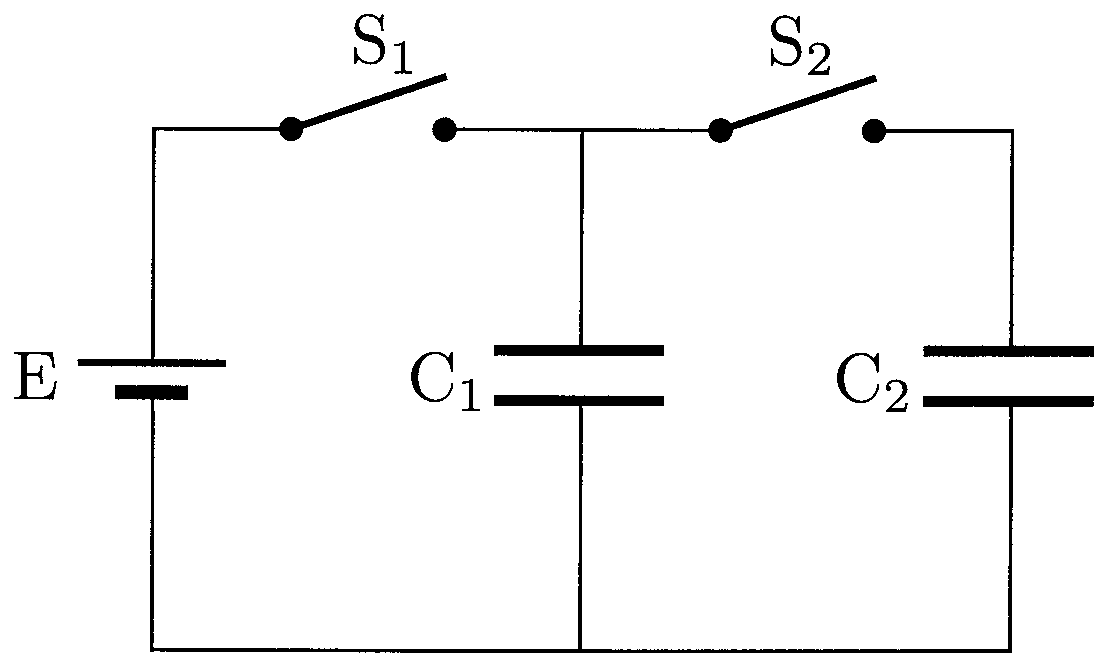
\includegraphics[keepaspectratio,width=62mm]{fig/n25_p51_zu.png}
\end{zuright}
\begin{komon}
\ko{1} $\mathrm{C}_1$に蓄えられている電気量$Q_0\U{C}$および静電エネルギー$U_0\U{J}$を求めよ．
\end{komon}
\hspace{1zw}次に$\mathrm{S}_1$を開き，$\mathrm{S}_2$を閉じる．
\begin{komon}
\ko{2} $\mathrm{C}_1$，$\mathrm{C}_2$に蓄えられている電気量$Q_1$，$Q_2\U{C}$を求めよ．
\ko{3} $\mathrm{C}_1$，$\mathrm{C}_2$全体の静電エネルギーの和の減少量を求めよ．
\end{komon}

\Mon[\Sitei]{直列回路}

\begin{zuright}{60mm}
\hspace{1zw}起電力がそれぞれ$V$，$\dfrac{1}{2}V\U{V}$の電池$\mathrm{E}_1$，$\mathrm{E}_2$，スイッチ$\mathrm{S}$，電気容量がそれぞれ$2C$，$C\U{F}$のコンデンサー$\mathrm{C}_1$，$\mathrm{C}_2$が右図のように接続されている．はじめ$\mathrm{C}_1$，$\mathrm{C}_2$には電荷が蓄えられていなかった．各スイッチ操作の後には十分時間を置くものとして，以下の設問に答えよ．
\par
\hspace{1zw}まず$\mathrm{S}$を$\mathrm{a}$側に接続した．
\zusep
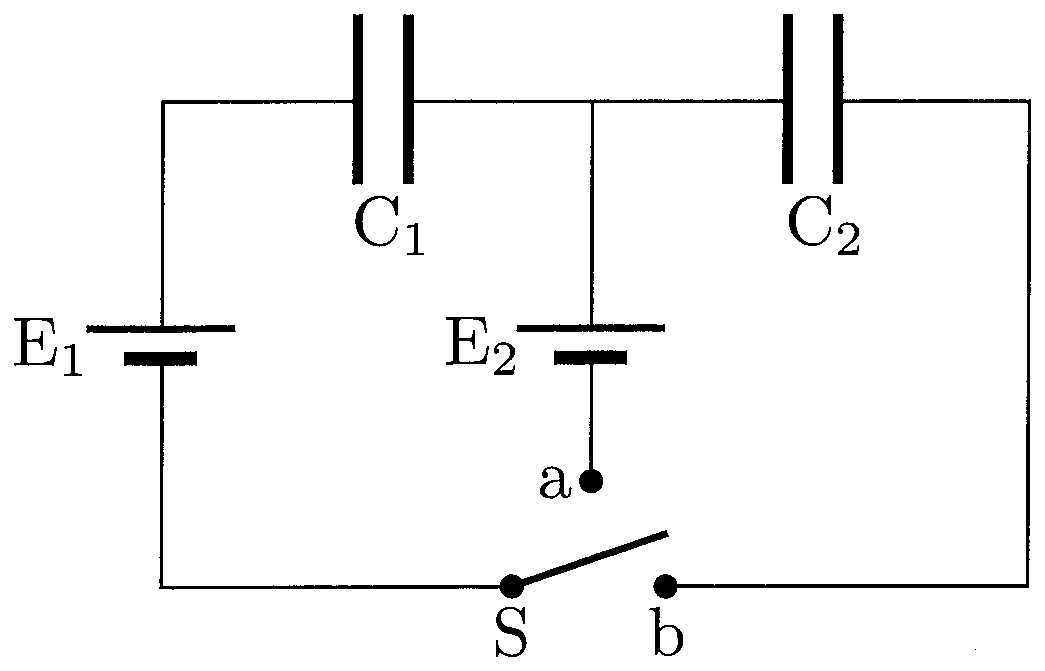
\includegraphics[keepaspectratio,width=60mm]{fig/n25_p52_zu.png}
\end{zuright}
\begin{komon}
\ko{1} $\mathrm{C}_1$に蓄えられる電気量$Q_0\U{C}$および静電エネルギー$U_0\U{J}$を求めよ．
\end{komon}
\hspace{1zw}次に$\mathrm{S}$を$\mathrm{b}$側に接続した．
\begin{komon}
\ko{2} $\mathrm{C}_1$，$\mathrm{C}_2$に蓄えられている電気量$Q_1$，$Q_2\U{C}$を求めよ．
\ko{3} $\mathrm{C}_1$，$\mathrm{C}_2$全体の静電エネルギーの和の変化量を求めよ．
\end{komon}

\Mon{コンデンサーの連結}

\begin{zuright}{58mm}
\hspace{1zw}電気容量がそれぞれ$2C$，$3C$，$5C\U{F}$のコンデンサー$\mathrm{C}_1$，$\mathrm{C}_2$，$\mathrm{C}_3$を右図のように起電力$V\U{V}$の電池$\mathrm{E}$に接続した．はじめ$\mathrm{C}_1$，$\mathrm{C}_2$，$\mathrm{C}_3$には電荷が蓄えられていなかった．この状態からスイッチ$\mathrm{S}$を閉じ，十分時間を置いた状態について，以下の設問に答えよ．
\begin{komon}
\ko{1} $\mathrm{C}_1$，$\mathrm{C}_2$，$\mathrm{C}_3$に蓄えられている電気量$Q_1$，$Q_2$，$Q_3\U{C}$を求めよ．
\ko{2} $\mathrm{C}_1$，$\mathrm{C}_2$，$\mathrm{C}_3$の両極板間の電位差$V_1$，$V_2$，$V_3\U{V}$を求めよ（大きさのみでよい）．
\end{komon}
\zusep
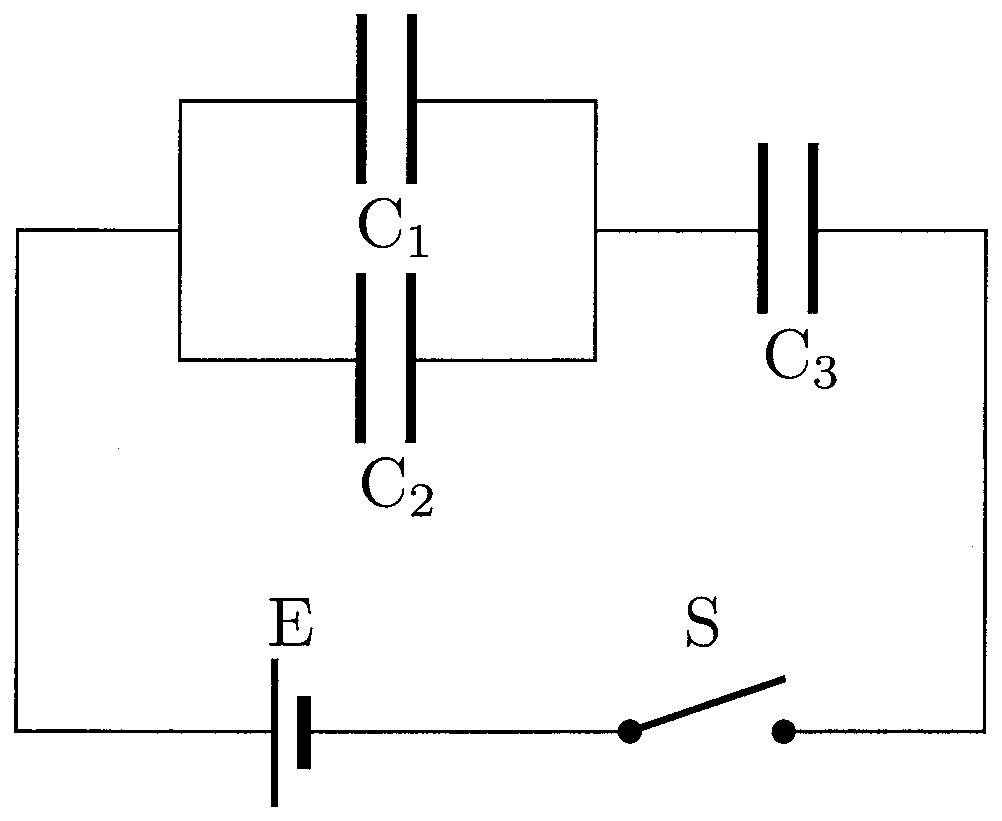
\includegraphics[keepaspectratio,width=58mm]{fig/n25_p53_zu.png}
\end{zuright}

\Mon[\Sitei]{コンデンサー回路のスイッチ操作}

\begin{zuright}{68mm}
\hspace{1zw}起電力$E\U{V}$の電池$\mathrm{E}$に，電気容量がそれぞれ$C$，$2C$，$3C\U{F}$のコンデンサー$\mathrm{C}_1$，$\mathrm{C}_2$，$\mathrm{C}_3$およびスイッチ$\mathrm{K}_1$，$\mathrm{K}_2$，検流計$\mathrm{G}$を右図のように接続し，$\mathrm{B}$点を接地しておく．はじめスイッチはいずれも開いており，すべてのコンデンサーについて電荷は蓄えられていなかった．
\zusep
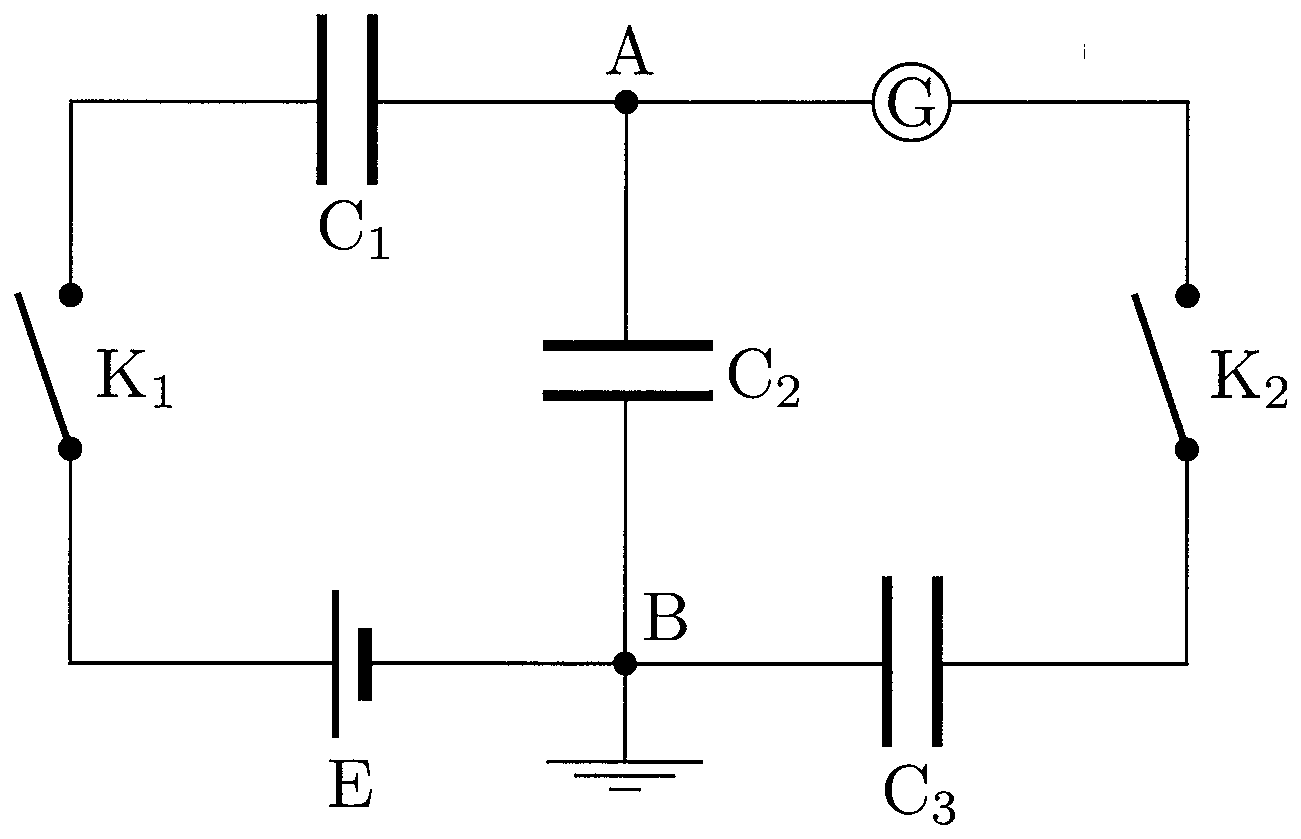
\includegraphics[keepaspectratio,width=68mm]{fig/n25_p54_zu.png}
\end{zuright}
\hspace{1zw}この状態から以下のようにスイッチを操作する．各スイッチの操作の後には十分な時間を置き，定常状態になってから電位を測るものとする．なお，検流計は通過した電気量を測る装置で，定常状態では検流計$\mathrm{G}$には電圧がかからないものとみなす．以下の設問に答えよ．
\begin{komon}
\ko{1} まず$\mathrm{K}_1$のみを閉じる．このときの$\mathrm{A}$点の電位を求めよ．
\ko{2} 次に，$\mathrm{K}_1$を開いてから$\mathrm{K}_2$を閉じた．このときの$\mathrm{A}$点の電位を求めよ．
\ko{3} (2)の操作で検流計$\mathrm{G}$を通過した電気量はいくらか．
\ko{4} さらに$\mathrm{K}_2$を開いてから$\mathrm{K}_1$を閉じた．このときの$\mathrm{A}$点の電位を求めよ．
\end{komon}

% ［55］は原本の【例題13】（再編案で例題→練習へ格下げ）．25.7 の直後に解く練習として置いた．
\Mon{複合極板コンデンサー}

\hspace{1zw}電気容量$C\U{F}$の平行平板コンデンサーに起電力$V\U{V}$の電池をつなぎ，両極板間に(1)〜(3)のように物質を入れたとき，コンデンサーに蓄えられる電気量をそれぞれ求めよ．
\begin{komon}
\ko{1} 極板間隔の半分の厚さの，帯電していない金属板を，極板と平行に中央に挿入した場合
\ko{2} 極板間の右半分を，比誘電率$\varepsilon_{\mathrm{r}}$の誘電体で満たした場合
\ko{3} 極板間の下半分を(2)と同じ誘電体で満たし，その誘電体の上面を，厚さの無視できる帯電していない金属板で覆った場合
\end{komon}
\begin{center}
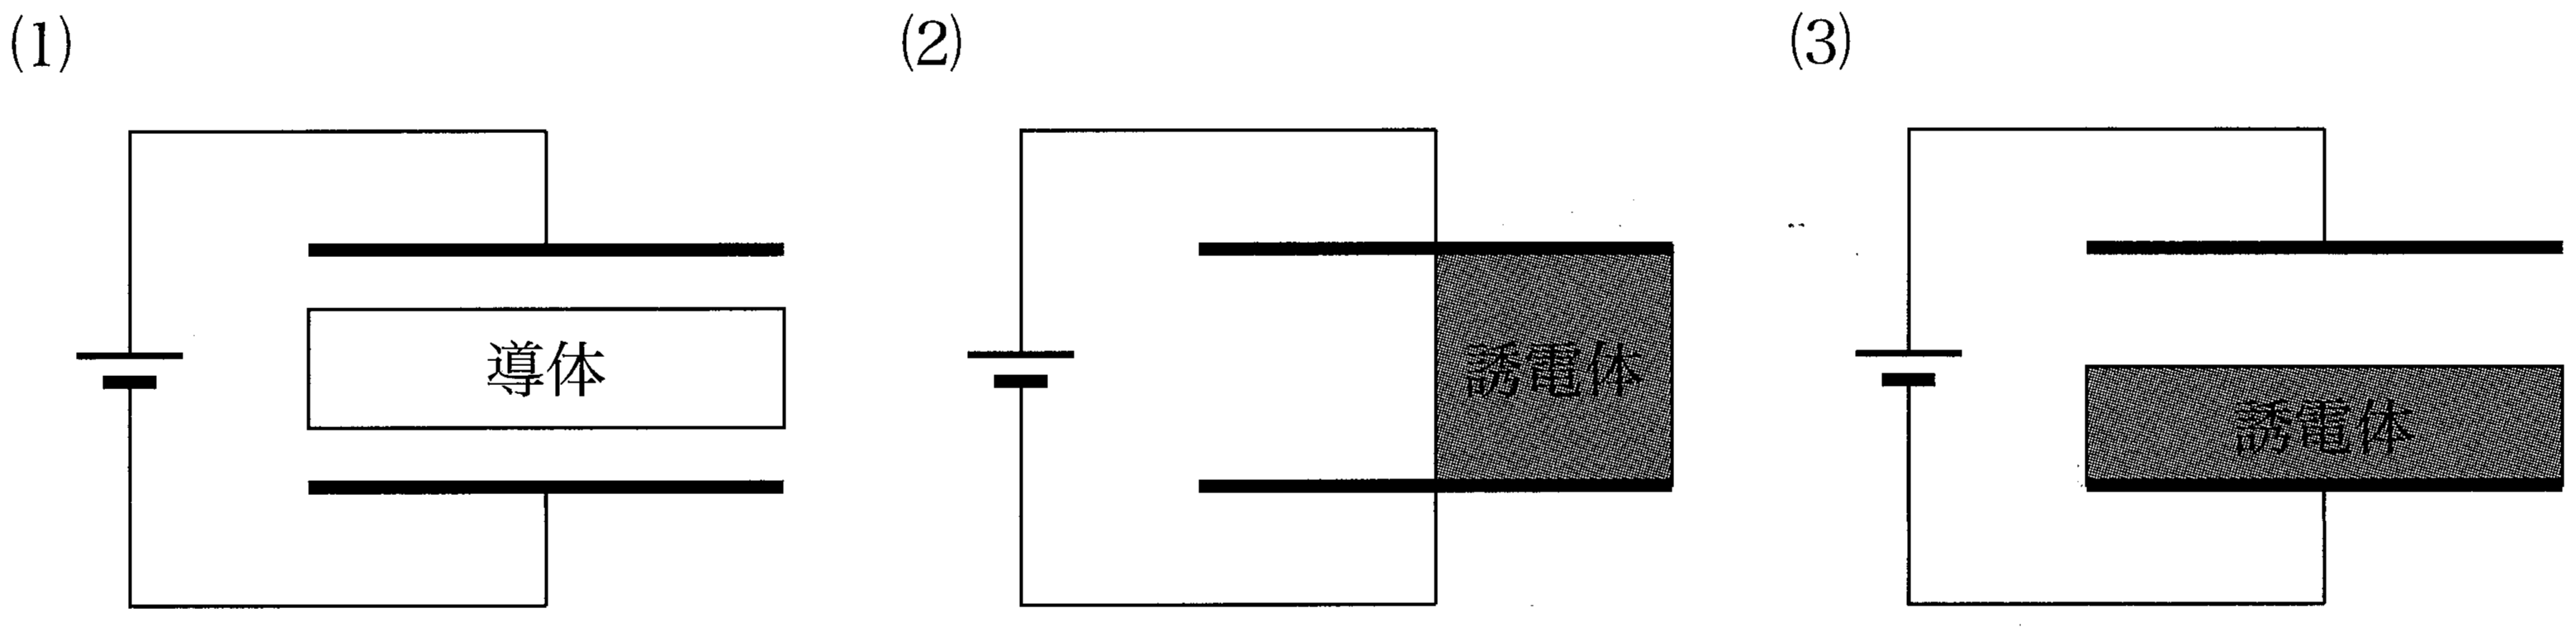
\includegraphics[keepaspectratio,width=150mm]{fig/n25_p55_zu.png}
\end{center}

\filbreak
\Rank{C問題}

\Mon{導体球の電気容量}

\hspace{1zw}次の文の空欄に入る適当な語句および式を示せ．ただし，電位の基準点は無限遠方に取るものとする．
\par
\hspace{1zw}孤立した球形の導体に正電荷$Q\U{C}$を与える場合について考えよう．この場合，同種の電荷同士は互いに\framebox[4zw]{\rule{0pt}{1.1zw}1}しあうので，電荷は球の\framebox[4zw]{\rule{0pt}{1.1zw}2}に分布する．導体球の表面は\framebox[4zw]{\rule{0pt}{1.1zw}3}面となるから，電気力線は球の表面に対して\framebox[4zw]{\rule{0pt}{1.1zw}4}に出ていく．このとき，導体球の内部には電気力線は作られないが，導体球の外側の電気力線の様子は，正電荷$Q\U{C}$が球の\framebox[4zw]{\rule{0pt}{1.1zw}5}に点電荷として存在しているときに作られる電気力線の様子と全く同じである．したがって球の表面および外側における電場，電位は点電荷の場合と同じように考えることができる．クーロンの法則の比例定数を$k\U{N\cdot m^2/C^2}$とすると，点電荷$Q\U{C}$から距離$r\U{m}$の点の電位は\framebox[4zw]{\rule{0pt}{1.1zw}6}であるから，半径$a\U{m}$の導体球の表面の電位は\framebox[4zw]{\rule{0pt}{1.1zw}7}となる．球の内部の電位はこの値\framebox[3zw]{\rule{0pt}{1.1zw}8}（\MARU{1}より大きい，\MARU{2}に等しい，\MARU{3}より小さい，から選べ）．
\par
\hspace{1zw}ここで，この導体球を一つの極板とみなし，さらに無限遠方をそれと対をなす仮想的な極板だとみなすと，これは電荷を蓄えるコンデンサーだとみなせる．このとき，このコンデンサーは$Q\U{C}$の電荷を蓄えており，極板間の電位差は\framebox[4zw]{\rule{0pt}{1.1zw}9}であるから，以上より導体球の電気容量$C\U{F}$は\framebox[4zw]{\rule{0pt}{1.1zw}10}であるとみなせる．

\Mon{誘電体と誘電分極}

\begin{zuright}{62mm}
\hspace{1zw}次の文の空欄に入る適当な語句および式を示せ．
\par
\hspace{1zw}誘電体（不導体，絶縁体とも呼ばれる）の場合，すべての電子は原子や分子に束縛されているため，金属の\framebox[4zw]{\rule{0pt}{1.1zw}1}とは異なり，電気伝導に寄与しない．今，極板面積$S\U{m^2}$，極板間距離$d\U{m}$の平行平板コンデンサーを2個用意する．一方のコンデンサー（以下$\mathrm{A}$と呼ぶ）の極板間は真空（誘電率$\varepsilon_0\U{C^2/N\cdot m^2}$）にし，他方のコンデンサー（以下$\mathrm{B}$と呼ぶ）の極板間を比誘電率$\varepsilon_{\mathrm{r}}$の誘電体で満たす．
\zusep
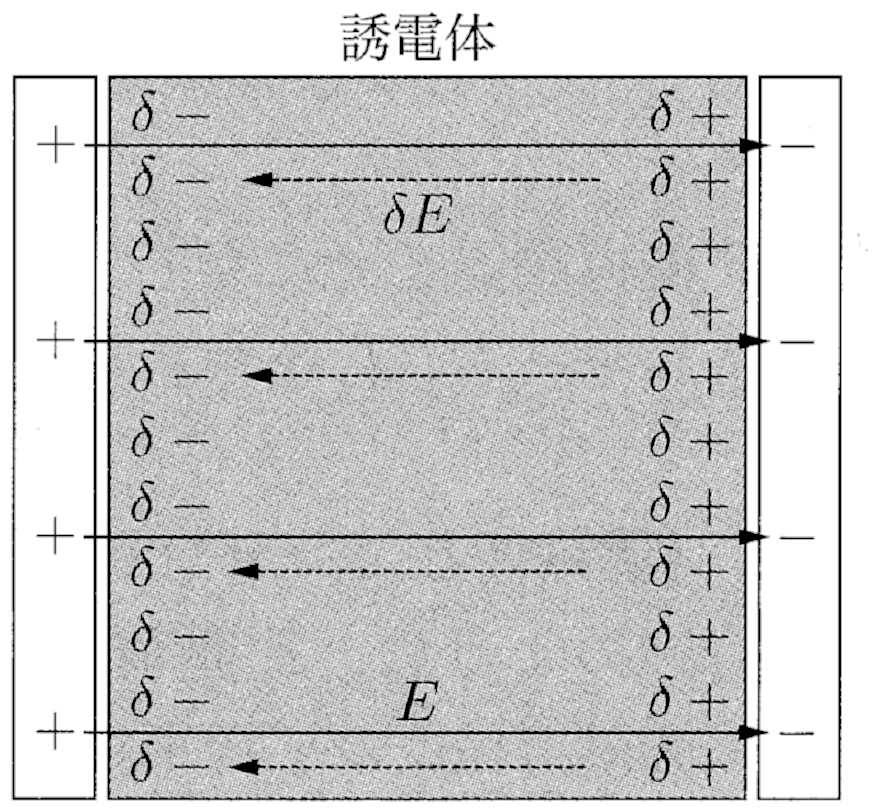
\includegraphics[keepaspectratio,width=62mm]{fig/n25_a57_zu0.png}
\end{zuright}
\hspace{1zw}これらのコンデンサーを起電力$V\U{V}$の電池にそれぞれ接続すると，極板間の電位差は電池により$V\U{V}$に保たれているので，コンデンサー$\mathrm{A}$，$\mathrm{B}$に蓄えられる電気量はそれぞれ\framebox[4zw]{\rule{0pt}{1.1zw}2}，\framebox[4zw]{\rule{0pt}{1.1zw}3}であり，極板間にはそれぞれ\framebox[4zw]{\rule{0pt}{1.1zw}4}，\framebox[4zw]{\rule{0pt}{1.1zw}5}の電場が生じている．このとき，$\mathrm{B}$のコンデンサーの極板上の電荷だけに着目すると，この電荷はガウスの法則を考えることにより極板間に強さが\framebox[4zw]{\rule{0pt}{1.1zw}6}の電場を作っている．しかし，コンデンサー$\mathrm{B}$のすき間を満たした誘電体で\framebox[4zw]{\rule{0pt}{1.1zw}7}と呼ばれる現象が起こり，その表面に発生する電荷が\framebox[4zw]{\rule{0pt}{1.1zw}6}の電場を弱めるような向きに電場を作るため，その結果，極板間の電場が\framebox[4zw]{\rule{0pt}{1.1zw}5}の値になる．よって，誘電体の表面に発生する電荷が作る電場の大きさは\framebox[4zw]{\rule{0pt}{1.1zw}8}であり，その電気量の大きさは\framebox[4zw]{\rule{0pt}{1.1zw}9}である．

\Mon{コンデンサーと静電エネルギー}

\begin{zuright}{70mm}
\hspace{1zw}起電力が$10V\U{V}$の電池$\mathrm{E}$，スイッチ$\mathrm{S}_1$，$\mathrm{S}_2$，抵抗$\mathrm{R}$，電気容量がそれぞれ$3C$，$2C$，$4C$，$6C\U{F}$のコンデンサー$\mathrm{C}_1$，$\mathrm{C}_2$，$\mathrm{C}_3$，$\mathrm{C}_4$が右図のように接続されている．はじめ$\mathrm{C}_1$，$\mathrm{C}_2$，$\mathrm{C}_3$，$\mathrm{C}_4$には電荷が蓄えられていなかった．各スイッチ操作の後には十分な時間を置くものとして，以下の設問に答えよ．
\par
\hspace{1zw}まず$\mathrm{S}_2$を開いたまま$\mathrm{S}_1$を閉じた．
\zusep
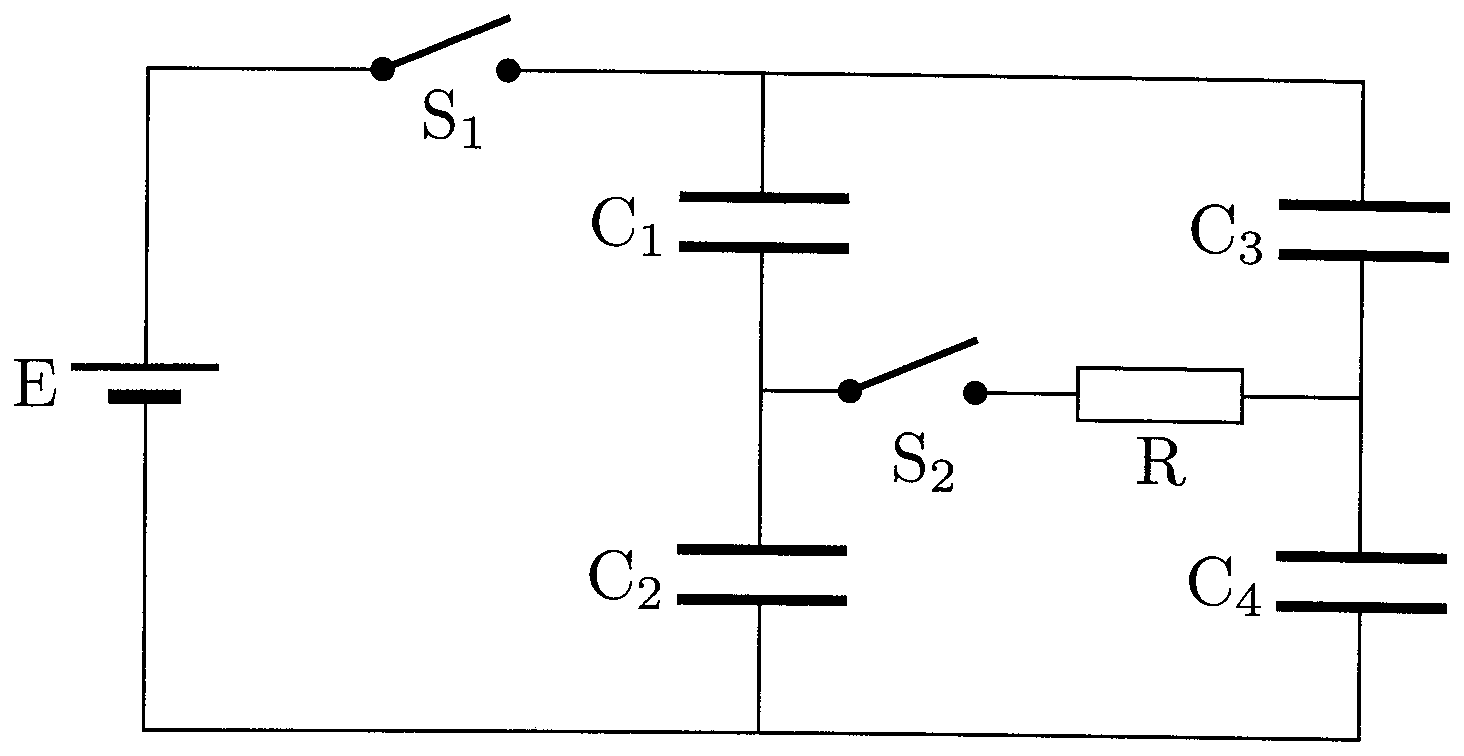
\includegraphics[keepaspectratio,width=70mm]{fig/n25_p58_zu.png}
\end{zuright}
\begin{komon}
\ko{1} 各コンデンサーの上側極板に蓄えられた電気量$Q_1$，$Q_2$，$Q_3$，$Q_4\U{C}$を求めよ．
\ko{2} 各コンデンサーに蓄えられた静電エネルギーの和$U\U{J}$を求めよ．
\end{komon}
\hspace{1zw}次に$\mathrm{S}_1$を開いてから続いて$\mathrm{S}_2$を閉じた．
\begin{komon}
\ko{3} 各コンデンサーの上側極板に蓄えられた電気量$Q_1^\prime$，$Q_2^\prime$，$Q_3^\prime$，$Q_4^\prime\U{C}$を求めよ．
\end{komon}

\Mon{多極板コンデンサー}

\begin{zuright}{62mm}
\hspace{1zw}極板$\mathrm{A}$，$\mathrm{B}$からなる間隔が$2d\U{m}$，電気容量が$\dfrac{1}{2}C\U{F}$の平行平板コンデンサーと，極板と同形で厚さの無視できる薄い金属板$\mathrm{D}$がある．右図のように，金属板$\mathrm{D}$を両極板$\mathrm{A}$，$\mathrm{B}$から等距離になるように置き，起電力$V\U{V}$の電池$\mathrm{E}$およびスイッチ$\mathrm{S}$を通して図のような回路を作った．はじめ，スイッチは開いており，各極板上に電荷は蓄えられていなかった．各スイッチ操作の後には十分な時間を置くものとして，以下の設問に答えよ．
\zusep
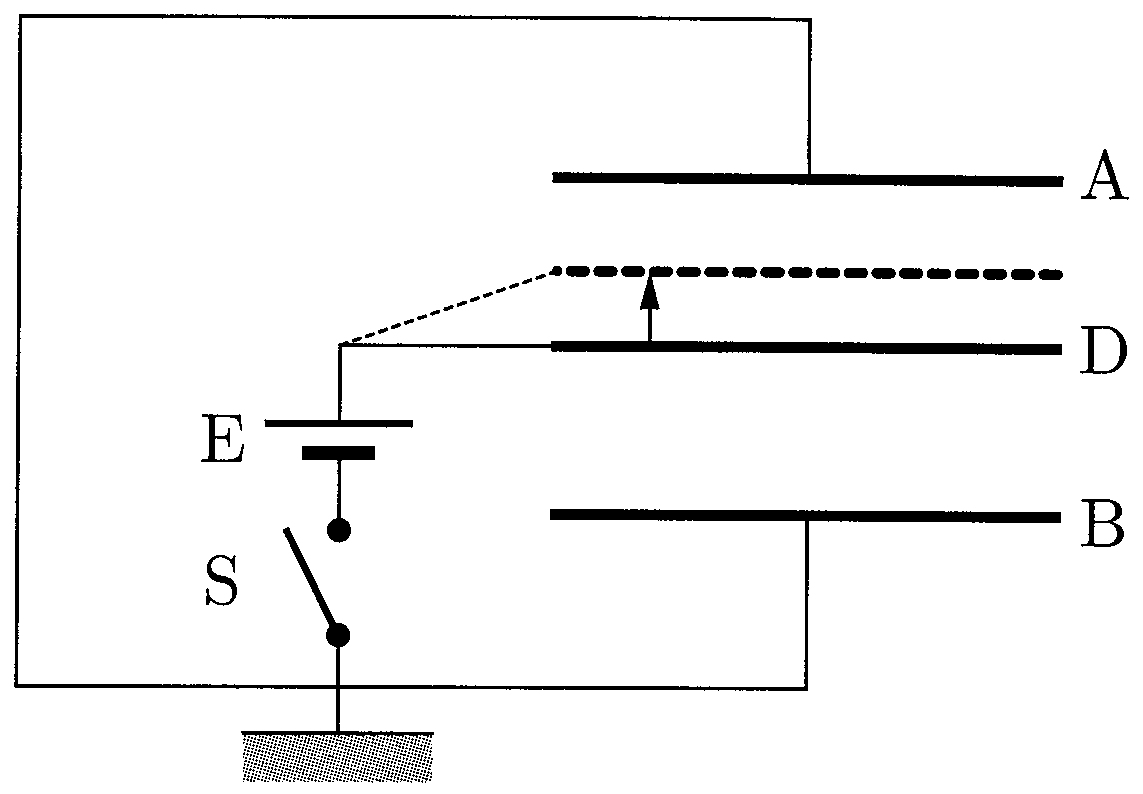
\includegraphics[keepaspectratio,width=62mm]{fig/n25_p59_zu.png}
\end{zuright}
\begin{komon}
\ko{1} まずスイッチ$\mathrm{S}$を閉じた．このとき，金属板$\mathrm{D}$に蓄えられる電気量$Q\U{C}$を求めよ．
\end{komon}
\hspace{1zw}次に，スイッチ$\mathrm{S}$を開き，その後，図の点線のように金属板$\mathrm{D}$を$\mathrm{A}$の方向に距離$x\U{m}$だけ移動した．
\begin{komon}
\ko{2} 極板$\mathrm{A}$，$\mathrm{B}$に蓄えられる電荷$Q_1$，$Q_2\U{C}$を求めよ．
\end{komon}

\newpage

%%%%%%%%%%%%%%%%%%%%  解答  %%%%%%%%%%%%%%%%%%%%
\KaiTitle{第25回　コンデンサーとコンデンサー回路}
\setlength{\columnseprule}{0.4pt}
\begin{multicols}{2}
\raggedcolumns

\Rank{A問題}
\MonN{47}{基本公式の確認}\par\nopagebreak
\begin{sisin}
(1)〜(6) $Q=CV$，$U=\dfrac{1}{2}CV^2=\dfrac{1}{2}QV=\dfrac{Q^2}{2C}$，$E=\dfrac{V}{d}$，$C=\varepsilon_0\dfrac{S}{d}$などを利用していく問題であるが，まずはこれらの式をきちんと暗記せよ．どの文字が何を表しているのか，どの文字の値が与えられているのかをよく考えながら適用していくこと．

「電圧」とは（極板間などの）電位差を意味する用語である．例えば電圧$1.5\U{V}$の電池とは，両端子の間の電位差が$1.5\U{V}$の電池を意味する．

マイクロ（$\mu$）は$10^{-6}$を表す．この機会に他の接頭語についても覚えておくこと．ミリ（m）は$10^{-3}$，マイクロ（$\mu$）は$10^{-6}$，ナノ（n）は$10^{-9}$，ピコ（p）は$10^{-12}$である．また，キロ（k）は$10^{3}$，メガ（M）は$10^{6}$，ギガ（G）は$10^{9}$，テラ（T）は$10^{12}$である．

(7)(8) コンデンサーの帯電量を求める問題では，どのような問題であろうとも，基本的には，\MARU{1}回路図を描いて適当な文字を用いて電荷分布を仮定する，\MARU{2}電荷保存の法則およびキルヒホッフの第二法則（コンデンサーにかかっている電圧と電池の起電力の関係式）を適用する，の流れで解くことができる．並列接続・直列接続の公式を用いて解くことも可能ではあるが，\underline{上述の}\hskip0pt\underline{攻め方で}\hskip0pt\underline{解けるよ}\hskip0pt\underline{うにして}\hskip0pt\underline{おくこと}．
\end{sisin}
\KaiHead
\begin{komon}
\ko{1} \[\begin{aligned}
         Q&=CV=1.5\times 10^{-6}\cdot 3.0\times 10^2\\
          &=4.5\times 10^{-4}\U{C}\Ans
       \end{aligned}\]
\ko{2} \[\begin{aligned}
         C&=\frac{Q}{V}=\frac{6.0\times 10^{-6}}{1.5}=4.0\times 10^{-6}\U{F}\\
          &=4.0\U{\mu F}\Ans
       \end{aligned}\]
\ko{3} $C=\varepsilon_0\dfrac{S}{d}\propto\dfrac{1}{d}$ゆえ，極板間隔に反比例する．よって，
       \[C^\prime=2C=2.0\U{\mu F}\Ans\]
\ko{4} \[\begin{aligned}
         E&=\frac{V}{d}=\frac{5.0}{2.5\times 10^{-3}}\\
          &=2.0\times 10^3\U{V/m}\Ans
       \end{aligned}\]
\ko{5} \[\begin{aligned}
         U&=\frac{1}{2}CV^2=\frac{1}{2}\cdot 2.0\times 10^{-6}\cdot 50^2\\
          &=2.5\times 10^{-3}\U{J}\Ans
       \end{aligned}\]
\ko{6} $C^\prime=\varepsilon\dfrac{S}{d}=\varepsilon_{\mathrm{r}}\cdot\varepsilon_0\dfrac{S}{d}=\varepsilon_{\mathrm{r}}C$ゆえ，
       \[\varepsilon_{\mathrm{r}}=\frac{C^\prime}{C}=\frac{6.0\times 10^{-6}}{2.0\times 10^{-6}}=3.0\]
       \hspace*{\fill}（単位はない）\Ans
\ko{7} \MARU{1}\ 電池を接続した場合の回路は次図のように書ける．このときの帯電量をそれぞれ$q_1\U{C}$，$q_2\U{C}$とおく．
       \begin{center}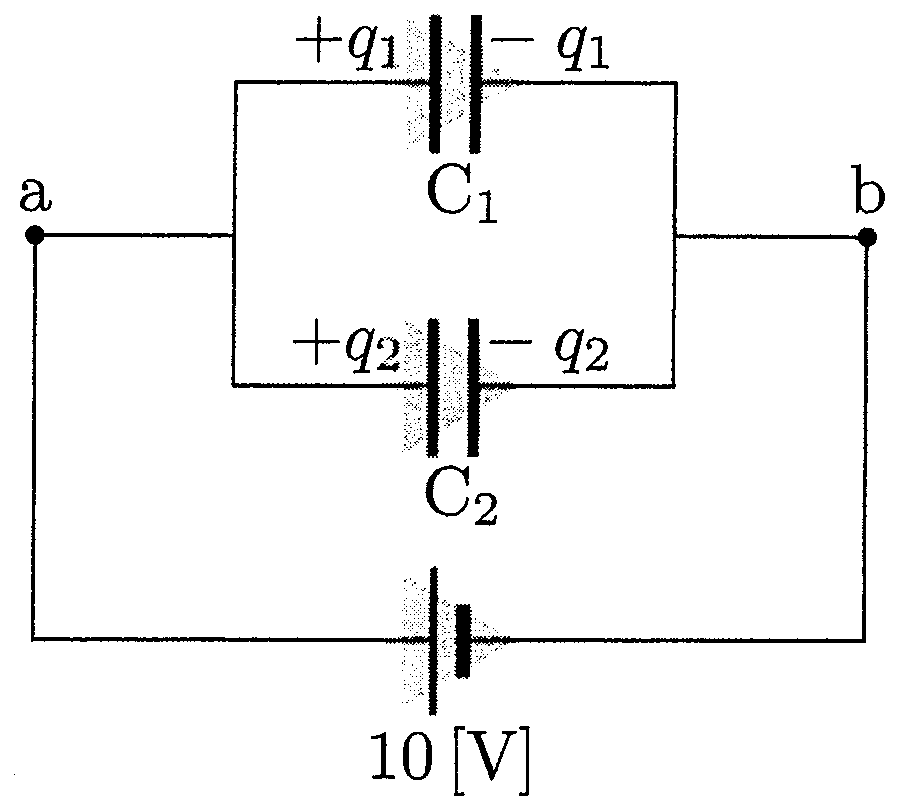
\includegraphics[keepaspectratio,width=58mm]{fig/n25_a47_zu1.png}\end{center}
       このとき，$\mathrm{C}_1$，$\mathrm{C}_2$にかかっている電圧は$10\U{V}$なので，
       \[q_1=6.0\times 10^{-6}\cdot 10,\quad q_2=6.0\times 10^{-6}\cdot 10\]
       が成立する．コンデンサー$\mathrm{C}_1$に蓄えられる電気量は
       \[q_1=6.0\times 10^{-5}\U{C}=6.0\times 10\U{\mu C}\Ans\]

       \MARU{2}\ 電池を接続した場合の回路は次図のように書ける．向かい合う極板には正負逆，大きさが同じ電荷が帯電すること，および図の点線部分（真ん中の部分）の電荷保存の法則（もともとコンデンサーには電荷がなかったので総電荷が$0$になる）を考えることにより，コンデンサー$\mathrm{C}_1$の左側極板の電荷を$+Q\U{C}$とおくと，図のような電荷分布になると考えられる．
       \begin{center}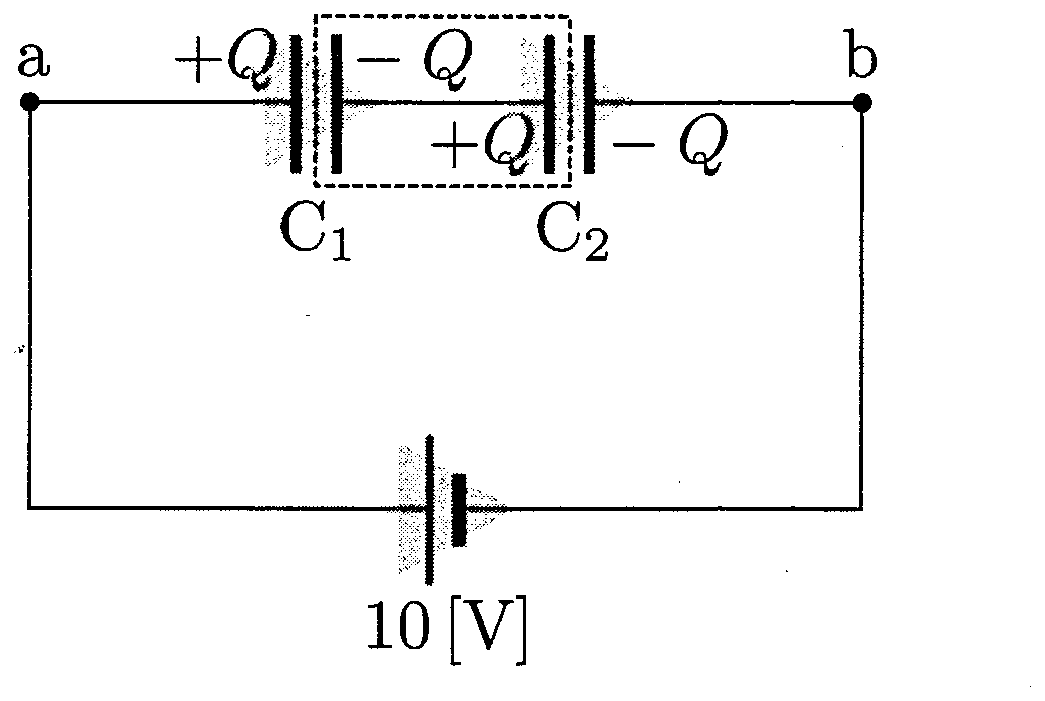
\includegraphics[keepaspectratio,width=58mm]{fig/n25_a47_zu2.png}\end{center}
       このとき，$\mathrm{C}_1$，$\mathrm{C}_2$にかかっている電圧の和が電池の起電力に等しいので，
       \[10=\frac{Q}{6.0\times 10^{-6}}+\frac{Q}{6.0\times 10^{-6}}\]
       これより，
       \[Q=3.0\times 10^{-5}\U{C}=3.0\times 10\U{\mu C}\Ans\]
\ko{8} 与えられたコンデンサーを分解し，それに対して電圧$V\U{V}$の電池を接続して考える．電気容量は極板面積に比例し，極板間隔に反比例し，誘電体を挟んだ場合は電気容量が比誘電率倍になることに注意して考えると，

       \MARU{1}\ このコンデンサーは，極板間隔が$\dfrac{2}{3}$倍になった真空コンデンサー$\mathrm{C}_1$（電気容量が$\dfrac{3}{2}$倍）と，極板間隔が$\dfrac{1}{3}$倍になった誘電体を挟んだコンデンサー$\mathrm{C}_2$（電気容量が$3\times 3$倍）との直列接続であるとみなせる．向かい合う極板には正負逆，大きさが同じ電荷が帯電すること，および図の点線部分（真ん中の部分）の電荷保存の法則（もともと誘電体の上面には電荷がなかったので総電荷が$0$になる）を考えることにより，コンデンサー$\mathrm{C}_1$の上側極板の電荷を$+Q\U{C}$とおくと，次図のような電荷分布になると考えられる．
       \begin{center}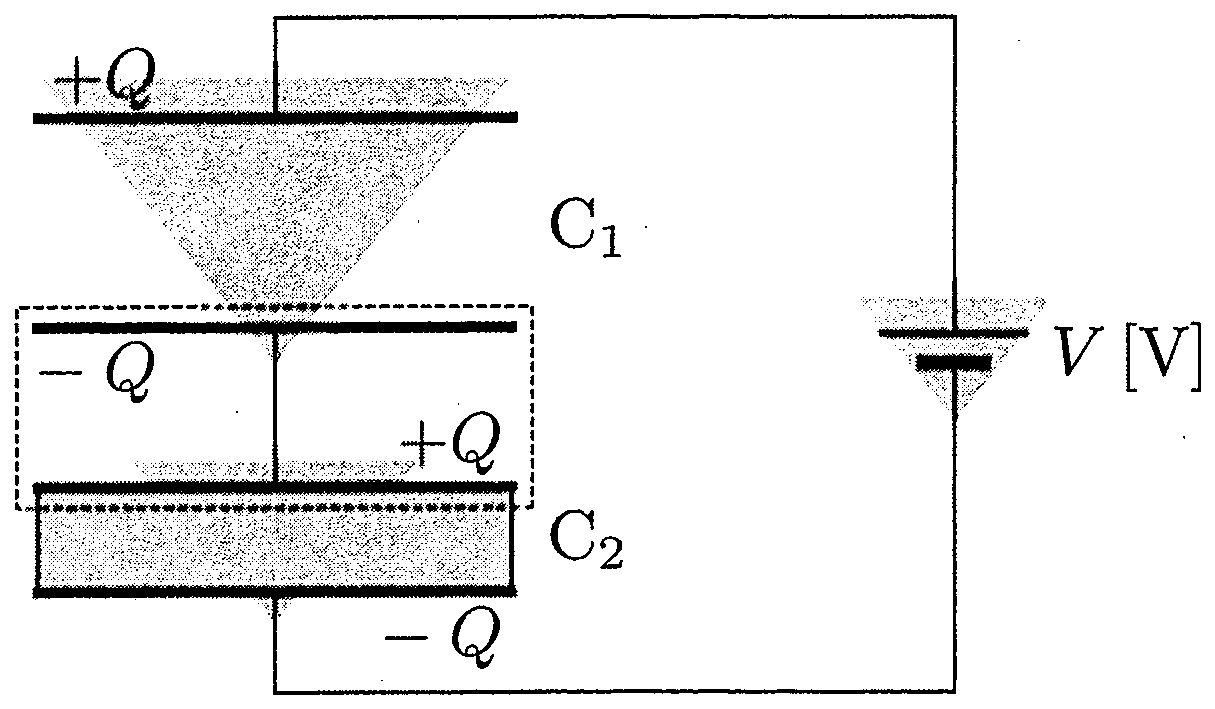
\includegraphics[keepaspectratio,width=56mm]{fig/n25_a47_zu3.png}\end{center}
       二つのコンデンサーにかかっている電圧の和が電池の起電力に等しいので，
       \[V=\frac{Q}{\frac{3}{2}C}+\frac{Q}{9C}\]
       となるのでこれを解いて，
       \[Q=\frac{9}{7}CV\U{C}\]
       である．求めるべき値は，コンデンサーの上側極板の帯電量であるから，
       \[+Q=+\frac{9}{7}CV\U{C}\Ans\]

       \MARU{2}\ このコンデンサーは，極板面積が$\dfrac{1}{2}$倍になった真空コンデンサー$\mathrm{C}_1$（電気容量が$\dfrac{1}{2}$倍）と，極板面積が$\dfrac{1}{2}$倍になった誘電体を挟んだコンデンサー$\mathrm{C}_2$（電気容量が$\dfrac{1}{2}\times 3$倍）との並列接続であるとみなせる．このときの帯電量をそれぞれ$q_1\U{C}$，$q_2\U{C}$とおく．
       \begin{center}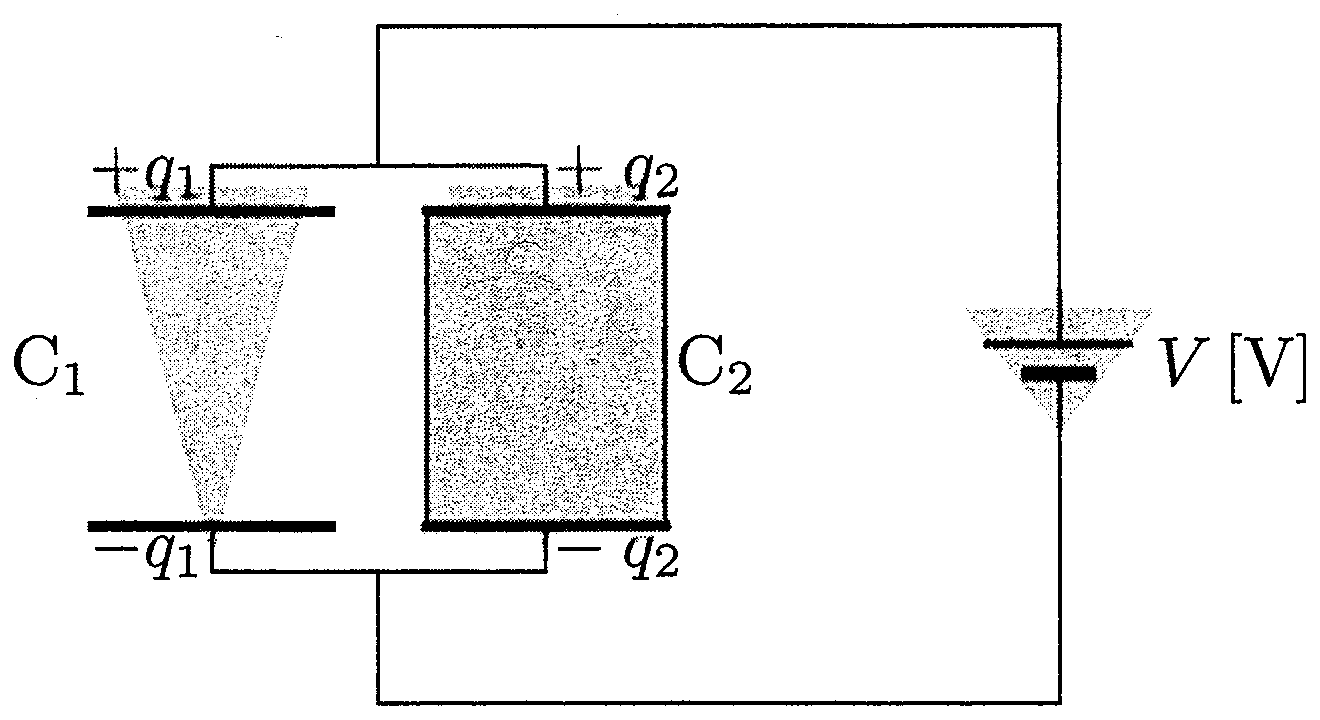
\includegraphics[keepaspectratio,width=58mm]{fig/n25_a47_zu4.png}\end{center}
       二つのコンデンサーにかかっている電圧はそれぞれ電池の起電力に等しいので，
       \[q_1=\frac{1}{2}CV\U{C},\quad q_2=\frac{3}{2}CV\U{C}\]
       と求められる．今，上のように回路を書き換える際には，もともとのコンデンサーの上側極板を，$\mathrm{C}_1$の上側部分と$\mathrm{C}_2$の上側部分とに分けて考えたので，もともとのコンデンサーの上側極板に蓄えられる電気量は，
       \[+q_1+q_2=2CV\U{C}\Ans\]
\end{komon}

\Rank{B問題}
\MonN{48}{平行平板コンデンサーの極板間隔の変化}\par\nopagebreak
\begin{sisin}
面積$S\U{m^2}$，間隔$d\U{m}$，極板間が真空の場合の平行平板コンデンサーの電気容量は$C=\varepsilon_0\dfrac{S}{d}\U{F}$となるが，この式から，\underline{電気容量}\hskip0pt\underline{は極板面}\hskip0pt\underline{積が大き}\hskip0pt\underline{いほど，}\hskip0pt\underline{また極板}\hskip0pt\underline{間隔が狭}\hskip0pt\underline{いほど大}\hskip0pt\underline{きくなる}（すなわち同じ電圧でもたくさんの電荷を蓄えることができる）ということが言える．このことは常識としておくこと．

またこのとき，極板間に生じる電場の強さは
\[E=\frac{V}{d}=\frac{Q}{\varepsilon_0 S}\U{V/m}\]
となり，これは{\gtfamily 蓄えられている電荷$Q$が変わらなければ極板間隔に依らない}ことを意味する．なぜなら，極板間の電場を作るのは極板上の電荷から上下に出される電気力線であり，その電気力線の様子は電荷$Q$が同じであれば極板間隔が変わっても不変だからである．

電気容量$C\U{F}$，極板間電圧$V\U{V}$，蓄えられている電荷$Q\U{C}$のコンデンサーのもつ静電エネルギーは$U=\dfrac{1}{2}CV^2\U{J}$であるが，$Q=CV$の式を利用すれば，
\[U=\frac{Q^2}{2C}=\frac{1}{2}QV=\frac{1}{2}CV^2\U{J}\]
と他の物理量を利用しても表すことができる．これらの式のうちのどれを利用すれば一番簡単に求められるのかを考えよ．

極板間隔を変化させる問題では，{\gtfamily 操作前後でどの量が変化せず，どの量が変化するのかを把握する}ことが重要である．{\gtfamily 問題文から明らかに変化しないと読み取れる物理量}（たいていは一つだけ）{\gtfamily 以外の量はすべて変化する可能性がある}ので，改めて上述した関係式を利用して一つずつ求めなければならない．

(2)では，電池を接続したまま極板間距離を変化させているので，コンデンサーにかかる電圧はずっと電池の電圧のまま操作前後で変化しない．

(3)では，電池を外して極板間距離を変化させているので，コンデンサーに蓄えられている電荷が操作前後で変化しない．
\end{sisin}
\KaiHead
\begin{komon}
\ko{1} 誘電率$\varepsilon_0$，面積$S$，極板間隔$d$なので，このコンデンサーの電気容量は，
       \[C=\varepsilon_0\frac{S}{d}\U{F}\Ans\]
       またコンデンサーにかかる電圧は$V\U{V}$であるから，蓄えられる電気量，静電エネルギーおよび極板間に生じる電場の強さは，
       \[Q=CV,\quad U=\frac{1}{2}CV^2,\quad E=\frac{V}{d}\]
       の関係式より，
       \[Q=\frac{\varepsilon_0SV}{d}\U{C},\quad U=\frac{\varepsilon_0SV^2}{2d}\U{J}\]
       \[E=\frac{V}{d}\U{V/m}\Ans\]
\ko{2} 極板間隔が$kd\U{m}$に変化したので，コンデンサーの電気容量は
       \[C^\prime=\varepsilon_0\frac{S}{kd}\U{F}\Ans\]
       に変化した．このとき，電池を接続したまま操作を行ったので，コンデンサーにかかる電圧は変化後も電池の電圧$V\U{V}$になる．よって，このときの各物理量は，
       \[Q^\prime=C^\prime V,\quad U^\prime=\frac{1}{2}C^\prime V^2,\quad E^\prime=\frac{V}{kd}\]
       などの関係式を利用して，
       \[Q^\prime=\frac{\varepsilon_0SV}{kd}\U{C},\quad U^\prime=\frac{\varepsilon_0SV^2}{2kd}\U{J}\]
       \[E^\prime=\frac{V}{kd}\U{V/m}\Ans\]
\ko{3} 前問と同様，極板間隔が$kd\U{m}$に変化したので，コンデンサーの電気容量は
       \[C^{\prime\prime}=\varepsilon_0\frac{S}{kd}\U{F}\Ans\]
       に変化した．このとき，電池を外してから極板間隔を変化させているので，コンデンサーに蓄えられた電気量が$Q\U{C}$のまま変わらなくなる．このときの極板間の電位差を$V^{\prime\prime}\U{V}$とすると（注：極板間の電位差は変わらないとはどこにも書かれていないので変化しうる物理量である），このときの各物理量の間には，
       \[Q=C^{\prime\prime}V^{\prime\prime},\quad U^{\prime\prime}=\frac{1}{2}C^{\prime\prime}V^{\prime\prime 2},\quad E^{\prime\prime}=\frac{V^{\prime\prime}}{kd}\]
       などの関係式が成立する．よってこれらを解いて，
       \[Q^{\prime\prime}=Q=\frac{\varepsilon_0SV}{d}\U{C},\quad U^{\prime\prime}=\frac{\varepsilon_0kSV^2}{2d}\U{J}\]
       \[E^{\prime\prime}=\frac{V}{d}\U{V/m}\Ans\]
\end{komon}
\begin{bekkai}
$U^{\prime\prime}$については，$U^{\prime\prime}=\dfrac{1}{2}C^{\prime\prime}V^{\prime\prime 2}\U{J}$の関係式を利用して求めようとすると$Q=C^{\prime\prime}V^{\prime\prime}$の式からいったん$V^{\prime\prime}$を求めなければならないため面倒である．このような場合には，
\[U^{\prime\prime}=\frac{Q^2}{2C^{\prime\prime}}\]
を利用すれば簡単に求めることができる．ただし，この式を利用する場合であっても，極板間の電位差が変わっていることに注意すること．また，指針でも述べたように，$E^{\prime\prime}$については，
\[\begin{aligned}
  E^{\prime\prime}&=\frac{V^{\prime\prime}}{kd}=\frac{Q/C^{\prime\prime}}{kd}=\frac{Q\cdot\frac{kd}{\varepsilon_0S}}{kd}\\
   &=\frac{Q}{\varepsilon_0S}
\end{aligned}\]
と変形してから求めるのも一つの手である．
\end{bekkai}

\MonN[\Sitei]{49}{コンデンサーの極板間の引力}\par\nopagebreak
\begin{sisin}
コンデンサーの二つの極板は，帯電すると正電荷・負電荷を持つため互いに引力を及ぼし合う．この引力は，コンデンサー極板間の間隔を微小変化させた際の静電エネルギー変化から求めることができ，これを考えるのが本問である．

本問から導かれる極板間引力の式
\[F=\frac{1}{2}QE\U{N}\]
は結果式として暗記しておくこと（25.2のまとめ枠）．
\end{sisin}
\KaiHead
真空の誘電率を$\varepsilon_0\U{C^2/N\cdot m^2}$，極板面積を$S\U{m^2}$とすると，極板間隔$d\U{m}$の最初の状態の電気容量は
\[C=\varepsilon_0\frac{S}{d}\U{F}\]
と表される．
\begin{komon}
\ko{1} スイッチ$\mathrm{K}$を閉じるとコンデンサーには$V\U{V}$の電圧がかかるので，
       \[\begin{aligned}
         &Q_0=CV\U{C}\\
         &U_0=\frac{Q_0^2}{2C}=\frac{1}{2}CV^2\U{J}\Ans
       \end{aligned}\]
\ko{2} スイッチ$\mathrm{K}$を開いたことにより，極板間隔を変化させても左側極板には$-Q_0=-CV\U{C}$が，右側極板には$+Q_0=+CV\U{C}$が蓄えられたままになり，これらが保存する．

       極板間隔を$3d\U{m}$にしたときの電気容量は，
       \[C_1=\varepsilon_0\frac{S}{3d}=\frac{1}{3}C\U{F}\]
       になるので，このときの静電エネルギーは
       \[U_1=\frac{Q_0^2}{2C_1}\]
       であり，各値を代入して，
       \[U_1=\frac{3}{2}CV^2\U{J}\Ans\]
       \begin{chuu}
       $U_1=\dfrac{1}{2}C_1V^2\U{J}$ではないことに注意．極板間隔を3倍にしたときにはもはや電池はつないでいないので，極板間の電位差は電池の電圧$V\U{V}$に等しいとは限らない（変化している）．
       \end{chuu}
\ko{3} (1)と(2)で求めた静電エネルギーを比較すると，
       \[U_1>U_0\]
       であるから，静電エネルギーは増加している．
       \begin{center}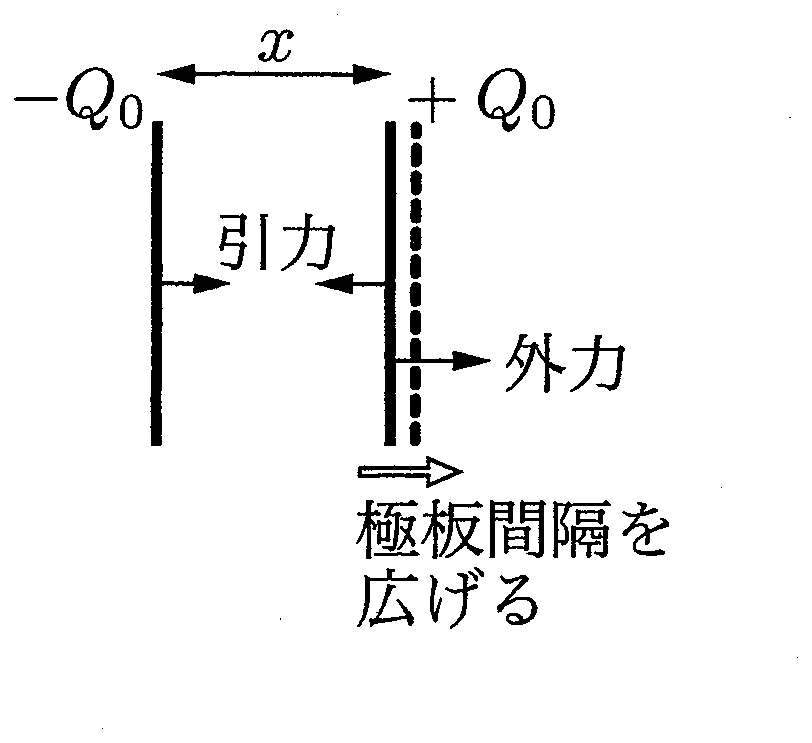
\includegraphics[keepaspectratio,width=50mm]{fig/n25_a49_zu1.png}\end{center}
       スイッチ$\mathrm{K}$を開くと左側極板には$-Q_0=-CV\U{C}$が，右側極板には$+Q_0=+CV\U{C}$が蓄えられたままになり，これらが保存するが，これらは逆符号の電荷であるから互いに引き合っている．よって極板間隔を広げるためには，この引力に逆らって外力を加えなければならない．ゆえに，この外力が極板を広げた際にした仕事が，静電エネルギーの増加としてコンデンサーに蓄えられる．\hspace*{\fill}\Ans
\ko{4} このコンデンサーに蓄えられている電荷は$Q_0=CV\U{C}$のまま変わらない．コンデンサーの極板間隔が$x\U{m}$のときのコンデンサーの電気容量は
       \[C(x)=\varepsilon_0\frac{S}{x}\U{F}\]
       であり，このときの静電エネルギーは
       \[U(x)=\frac{Q_0^2}{2C(x)}=\frac{Q_0^2x}{2\varepsilon_0S}\U{J}\]
       である．極板間隔をさらに$dx\U{m}$だけ広げた際の電気容量は
       \[C(x+dx)=\varepsilon_0\frac{S}{x+dx}\U{F}\]
       であり，このときの静電エネルギーは
       \[U(x+dx)=\frac{Q_0^2(x+dx)}{2\varepsilon_0S}\U{J}\]
       である．よって，極板間隔を変化させたときの静電エネルギーの増加量$dU$は，
       \[dU=U(x+dx)-U(x)=\frac{Q_0^2}{2\varepsilon_0S}dx\U{J}\]
       であり，これに$Q_0=CV\U{C}$，$C=\varepsilon_0\dfrac{S}{d}\U{F}$を代入して，
       \[dU=\frac{CV^2}{2d}dx\U{J}\Ans\]
\ko{5} 極板間隔を広げるために加える外力の大きさを$f(x)\U{N}$とすると，このときに極板に作用する力は次図の通り．
       \begin{center}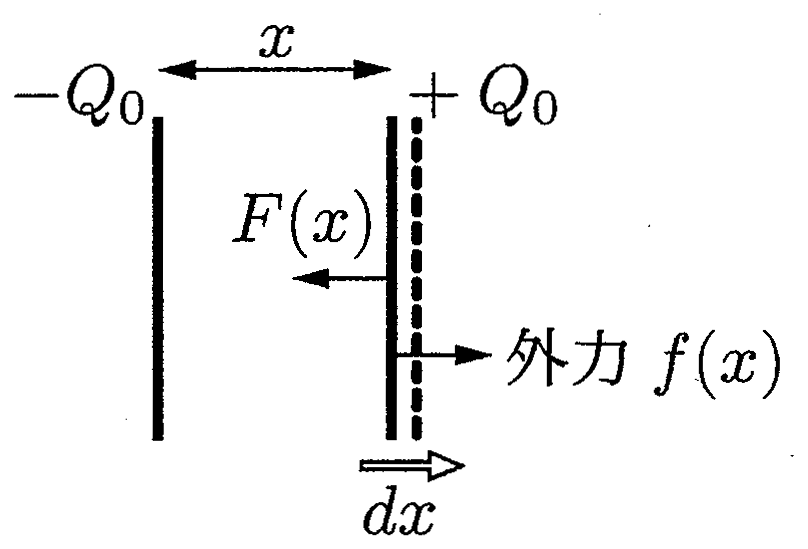
\includegraphics[keepaspectratio,width=52mm]{fig/n25_a49_zu2.png}\end{center}
       ゆっくりと極板を移動させるので，極板に作用する力がつり合いを保ちつつ極板が移動する．よって，力のつり合いより，
       \[F(x)=f(x)\]
       が成立する．

       極板間隔を$dx\U{m}$だけ広げるとき，この外力$f(x)$が極板に対してなす仕事は，仕事の定義式より$f(x)\cdot dx\cdot\cos 0^\circ\U{J}$であり，この仕事が(4)で求めた静電エネルギーの増加に利用されるので，
       \[dU=f(x)\cdot dx\cdot\cos 0^\circ\]
       が成立する．以上を整理して，
       \[f(x)=\frac{CV^2}{2d}\U{N}\]
       であるから，極板間引力は
       \[F(x)=\frac{CV^2}{2d}\U{N}\Ans\]
\ko{6} (5)のときの極板間の電位差$V(x)$および極板間の電場の強さ$E(x)$は，
       \[V(x)=\frac{Q_0}{C(x)},\quad E(x)=\frac{V(x)}{x}\]
       の2式より，
       \[E(x)=\frac{Q_0}{\varepsilon_0S}\U{V/m}\]
       である．$Q_0=CV\U{C}$，$C=\varepsilon_0\dfrac{S}{d}\U{F}$であるから(5)の答えを変形すると，
       \[F(x)=\frac{CV^2}{2d}=\frac{Q_0^2}{2dC}=\frac{Q_0^2}{2\varepsilon_0S}\U{N}\Ans\]
       また，さらに変形すると，
       \[F(x)=\frac{1}{2}Q_0E(x)\U{N}\Ans\]
       \begin{bsHosoku}{参考}
       (6)の答え$F(x)=\dfrac{Q_0^2}{2\varepsilon_0S}\U{N}$から分かるように，{\gtfamily 極板上の電荷が同じであれば，極板間隔が変化しても極板間引力は不変である}．
       \end{bsHosoku}
\ko{7} 一方，$\mathrm{K}$を閉じたまま極板間隔を$3d\U{m}$にした場合には，電池が接続されたままであるから極板上の電荷は変化し，極板間には電圧$V\U{V}$がかかったままになる．よって，電気容量$C_1=\dfrac{1}{3}C\U{F}$のコンデンサーに電圧$V\U{V}$がかかることになるので，このときに蓄えられる静電エネルギーは
       \[U_2=\frac{1}{2}C_1V^2=\frac{1}{6}CV^2\U{J}\Ans\]
       \begin{bsHosoku}{参考}
       (5)において，外力がなした仕事が静電エネルギー増加になると述べたが，極板間引力$F(x)=\dfrac{CV^2}{2d}\U{N}$のする仕事は考えなくてよい．なぜなら，この極板間引力は保存力であり，静電エネルギーに基づいて生じる力だからである．一般に，位置エネルギーに基づいて生じる力と，位置エネルギーとの間には（向きを含めて）
       \[F(x)=-\frac{dU}{dx}\]
       の関係があり，この式を用いても(5)の極板間引力を求めることが可能である．極板間隔が$x\U{m}$のときの静電エネルギーは
       \[U(x)=\frac{Q_0^2}{2C(x)}=\frac{Q_0^2x}{2\varepsilon_0S}\U{J}\]
       であるから，これより極板間引力は
       \[F(x)=-\frac{dU}{dx}=-\frac{Q_0^2}{2\varepsilon_0S}\U{N}\]
       % 原本はここの単位が [J] になっているが，力なので [N] が正しい（誤植）．
       となり，確かに(5)から求まる答えに一致する（マイナス符号は$x$が減少する向きであることを意味する）．
       \end{bsHosoku}
\end{komon}

\MonN[\Sitei]{50}{誘電体とコンデンサー}\par\nopagebreak
\begin{sisin}
一般に，エネルギーは小さい方が安定な状態に対応する．誘電体を入れた状態の時の方が静電エネルギーが小さくなるということは，誘電体は極板間にあった方が安定であるということを意味する．

また，自然界はなるべく安定な状態になろうとする性質を持つから，\underline{誘電体は}\hskip0pt\underline{極板間に}\hskip0pt\underline{引き込ま}\hskip0pt\underline{れる方向}\hskip0pt\underline{に力を受}\hskip0pt\underline{ける}（25.3）．
\end{sisin}
\KaiHead
\begin{komon}
\ko{1} この誘電体の誘電率は$\varepsilon=\varepsilon_{\mathrm{r}}\cdot\varepsilon_0\U{C^2/N\cdot m^2}$であるから，このコンデンサーの電気容量は
       \[C=\varepsilon\frac{S}{d}=\varepsilon_{\mathrm{r}}\varepsilon_0\frac{S}{d}\U{F}\]
       このコンデンサーには電池によって$V\U{V}$の電圧がかかっているので，蓄えられる電気量は，
       \[Q_0=CV=\frac{\varepsilon_{\mathrm{r}}\varepsilon_0SV}{d}\U{C}\Ans\]
\ko{2} (1)のときの静電エネルギーは
       \[U_0=\frac{Q_0^2}{2C}=\frac{\varepsilon_{\mathrm{r}}\varepsilon_0SV^2}{2d}\U{J}\]
       である．

       誘電体を引き抜いた後のコンデンサーの電気容量$C_0$は，
       \[C_0=\varepsilon_0\frac{S}{d}\U{F}\]
       になる．

       スイッチ$\mathrm{K}$を開くと上側極板には$+Q_0\U{C}$が，下側極板には$-Q_0\U{C}$が蓄えられたままになり，これらが保存する．よってこのときの静電エネルギーは，
       \[U_1=\frac{Q_0^2}{2C_0}=\frac{\varepsilon_{\mathrm{r}}^2\varepsilon_0SV^2}{2d}\U{J}\]
       である．この二つの静電エネルギーの大小を比較すると，$\varepsilon_{\mathrm{r}}$は必ず$1$より大きくなることに注意すると，
       \[U_1-U_0=(\varepsilon_{\mathrm{r}}-1)\frac{\varepsilon_{\mathrm{r}}\varepsilon_0SV^2}{2d}\U{J}\Ans\]
       であり，これは正の値であるから静電エネルギーは増加している．

       この答えより，誘電体を入れた状態の時の方が静電エネルギーが小さくなるので，誘電体は極板間にあった方が安定である．よって，誘電体は極板間に引き込まれる方向に力を受けるので，誘電体を引きずり出すためにはこの力に逆らって外力を加える必要がある．よって，誘電体を引きずり出すために加えた外力がした仕事によって，静電エネルギーが増加した．\hspace*{\fill}\Ans
\ko{3} 再び$\mathrm{K}$を閉じるとコンデンサーには再び電池の電圧$V\U{V}$がかかるので，極板には，
       \[Q_1=C_0V=\frac{\varepsilon_0SV}{d}\U{C}\]
       の電荷が蓄えられる．上側の極板に着目すると，スイッチ$\mathrm{K}$を閉じる前と後で，その電荷は
       \[+Q_0=+\frac{\varepsilon_{\mathrm{r}}\varepsilon_0SV}{d}\U{C}\]
       から，
       \[+Q_1=+\frac{\varepsilon_0SV}{d}\U{C}\]
       へと変化（減少）している．その減少分はスイッチ$\mathrm{K}$を左向きに通過して下側極板の側へ移動したと考えられる．よって，通過した電気量は，
       \[Q_0-Q_1=(\varepsilon_{\mathrm{r}}-1)\frac{\varepsilon_0SV}{d}\U{C}\]
       であり，これだけの電荷が$\mathrm{K}$を左向きに通過した．\hspace*{\fill}\Ans
\end{komon}

\MonN{51}{並列接続}\par\nopagebreak
\begin{sisin}
この先，［51］〜［59］でコンデンサー回路のスイッチ切り替え問題について扱うが，その基本的取り扱いはすべての問題について共通であり，このやり方さえ覚えておけば（手間はともかくとして）どんな回路，どんなスイッチ切り替えについてもその帯電量を求めることができる．この方法をきっちりとマスターしておくこと．

\MARU{1} スイッチ切り替え前と切り替え後の回路図を書き出して，スイッチ切り替え前の各極板の帯電量を書き込んでおく．

\MARU{2} 次に，スイッチ切り替え後の各極板の帯電量を適当な文字で仮定する．この際，向かい合う極板には必ず正負逆，同じ大きさの電荷が帯電することに注意する．また，極板の高電位の側に正電荷が帯電するが，回路によってはどちらの極板の方が電位が高いかが分からないこともある．このような場合は，とりあえず適当にカンで，電位が高くなるだろうと思った方をプラスとして文字設定を行っておく（間違っていた場合は，文字の中味がマイナスになるような答えが出てくるのですぐに分かる）．

\MARU{3} それぞれの極板間の電位差を求め，回路の閉ループ部分それぞれに対してキルヒホッフの第二法則を用いる．例えば本問の場合，左側のループ，右側のループ，回路をぐるりと回る外周のループの三つが考えられるが，数学的に独立な方程式はこれらのうち二つしかなく，もう一つはその二つの式の足し合わせなどの数学的変形によって導ける．

\MARU{4} スイッチ操作前後の図を見比べた際に，回路の他の部分と接続していない部分を見つけ出し，その部分に対して電荷保存の法則を適用する．

\MARU{5} あとは\MARU{3}，\MARU{4}を解く（ただの計算問題である）．

指針そのものは決して難しくないが，コンデンサー回路問題はある程度の慣れを要求される．横着せずにスイッチ操作\underline{前後の図}\hskip0pt\underline{の両方を}\hskip0pt\underline{ひとつず}\hskip0pt\underline{つ書き出}\hskip0pt\underline{し}，それに対して帯電量を書き込んで考えれば，コンデンサー回路問題は入試問題といえど易問である．
\end{sisin}
\KaiHead
\begin{komon}
\ko{1} スイッチの操作前後の回路図は下の通りである．この際，スイッチ$\mathrm{S}_2$は開いたままであるから，コンデンサー$\mathrm{C}_2$の上側極板については点線で囲んだ枠内の電荷保存の法則を考えると$0\U{C}$のまま変化しないので，それに向かい合う$\mathrm{C}_2$の下側極板の帯電量も$0\U{C}$である．$\mathrm{C}_1$は明らかに上側極板の方が電位が高いので，上側極板の帯電量が$+Q_0\U{C}$，下側極板の帯電量が$-Q_0\U{C}$である．
       \begin{center}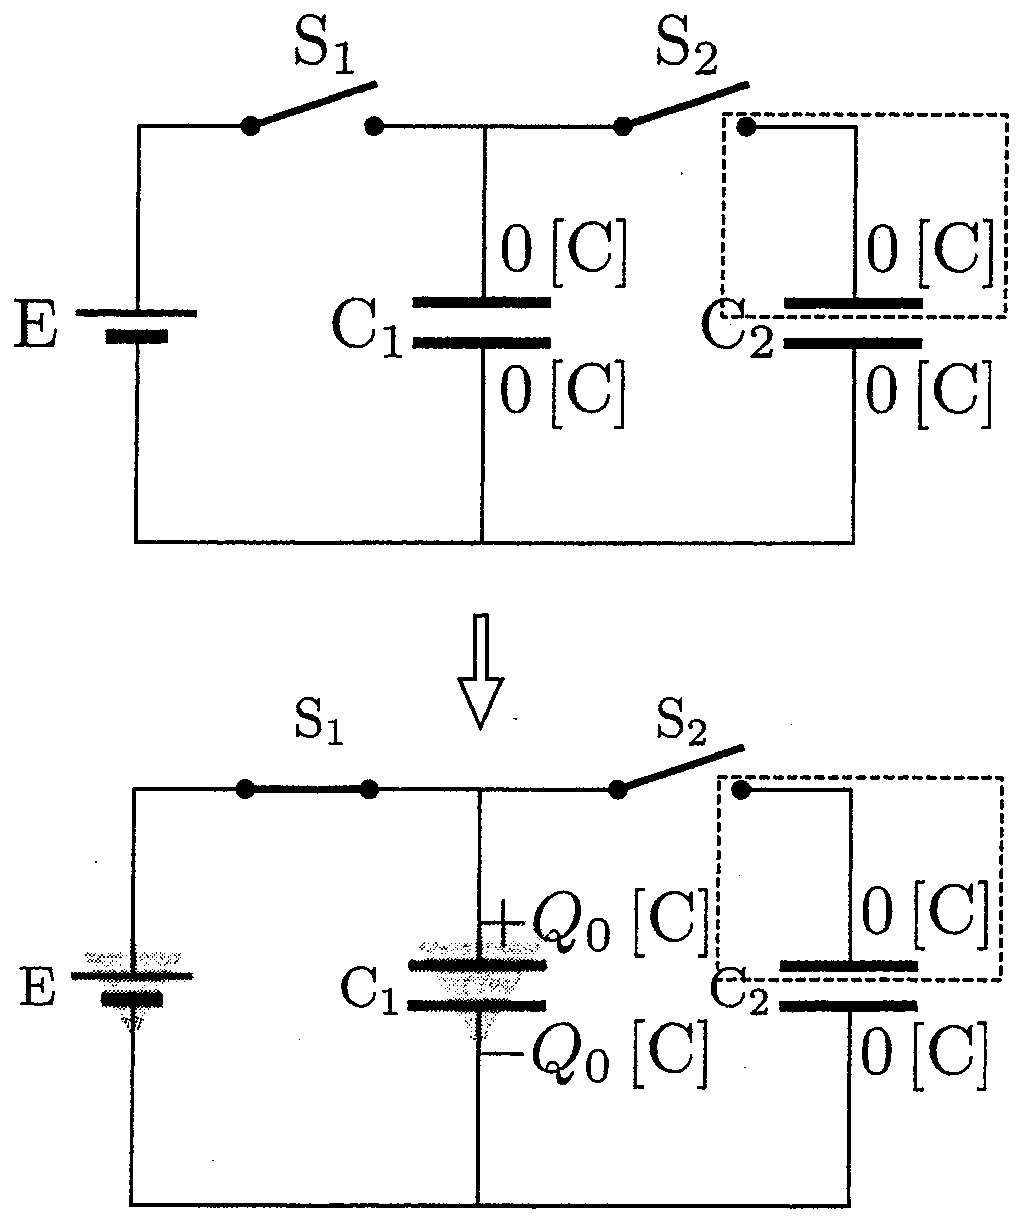
\includegraphics[keepaspectratio,width=60mm]{fig/n25_a51_zu1.png}\end{center}
       このとき，閉ループを作っているのは左側の部分だけであり，このループに対してキルヒホッフの第二法則を用いると，
       \[V=\frac{Q_0}{2C}\]
       である．よってこれを解いて，
       \[Q_0=2CV\U{C}\Ans\]
       またこのとき，$\mathrm{C}_1$に蓄えられている静電エネルギーは，
       \[U_0=\frac{1}{2}\cdot\frac{Q_0^2}{2C}=CV^2\U{J}\Ans\]
\ko{2} $\mathrm{S}_1$を開いても電荷は移動しないので，$\mathrm{S}_1$を開いた状態での帯電状態は次図のようになる．
       \begin{center}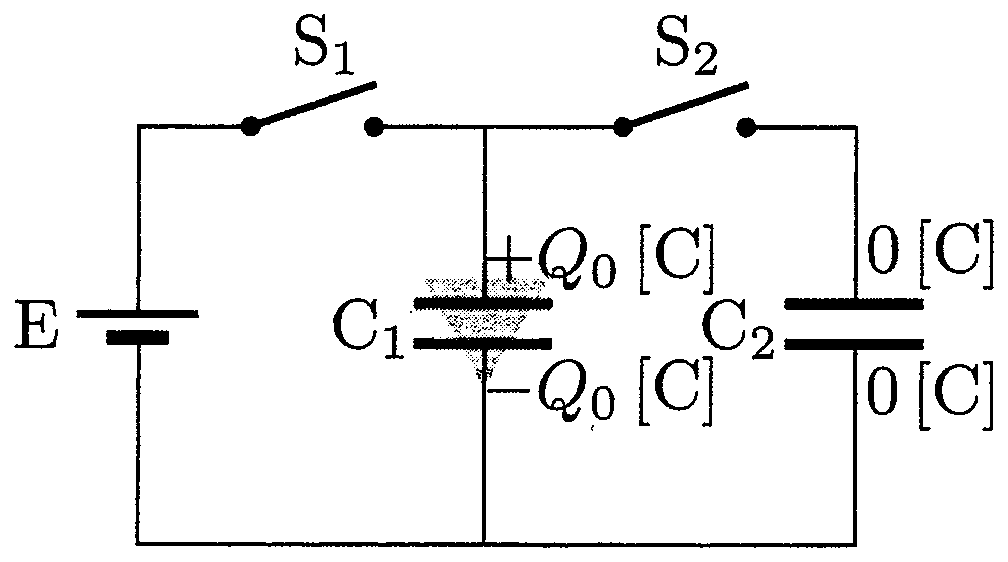
\includegraphics[keepaspectratio,width=58mm]{fig/n25_a51_zu2.png}\end{center}
       この状態からスイッチ$\mathrm{S}_2$を閉じると，コンデンサー$\mathrm{C}_2$に対して電圧がかかるため，電荷が移動して新しい電荷分布となる．各コンデンサーの上側極板に帯電する電気量をそれぞれ$+Q_1\U{C}$，$+Q_2\U{C}$とおくと，スイッチ操作前後の帯電状態は次図のように変化する．
       \begin{center}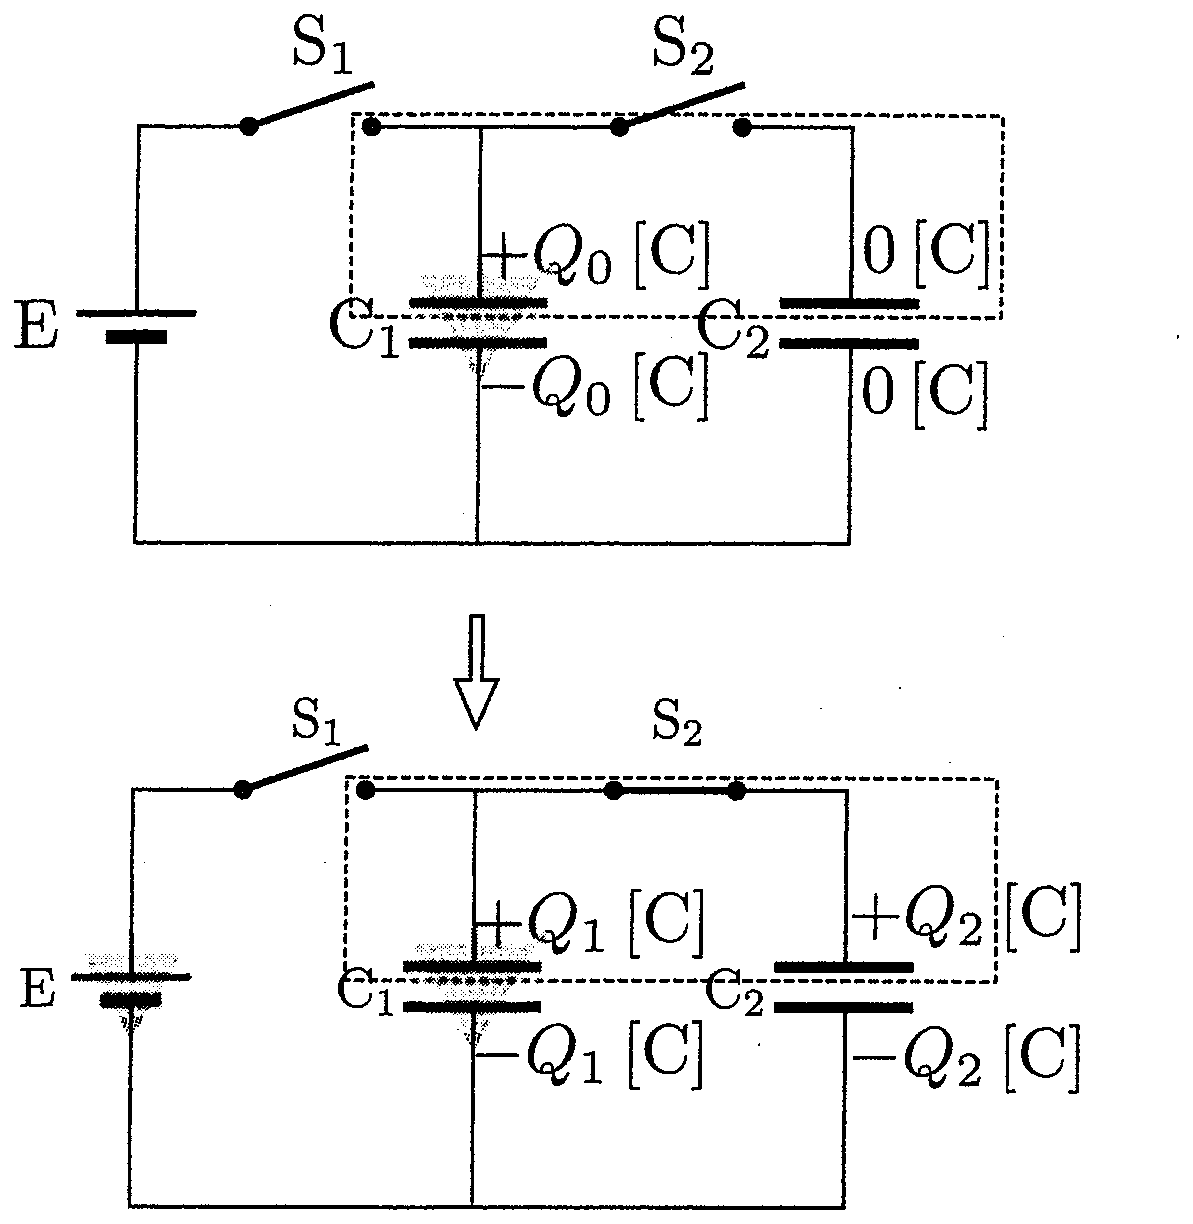
\includegraphics[keepaspectratio,width=60mm]{fig/n25_a51_zu3.png}\end{center}
       このとき，閉ループを作っているのは右側の部分だけであり，このループに対してキルヒホッフの第二法則を用いると，
       \[0=\frac{Q_1}{2C}-\frac{Q_2}{C}\]
       である．また，図の点線の四角枠囲み部分に着目すると，ここはスイッチ操作前後について，回路の他の部分と接続していない部分である．よって，この部分に対して電荷保存の法則を適用すると，
       \[+Q_0+0=+Q_1+Q_2\]
       である．以上2式および(1)の答えを用いて計算すると，
       \[Q_1=\frac{4}{3}CV\U{C},\quad Q_2=\frac{2}{3}CV\U{C}\Ans\]
\ko{3} (2)の終状態での静電エネルギーの総和は，
       \[U_1=\frac{1}{2}\cdot\frac{Q_1^2}{2C}+\frac{1}{2}\cdot\frac{Q_2^2}{C}=\frac{2}{3}CV^2\U{J}\]
       であるから，全体の静電エネルギーの減少量は，
       \[\left(U_0+\frac{1}{2}\cdot\frac{0^2}{C}\right)-U_1=\frac{1}{3}CV^2\U{J}\Ans\]
       \begin{bsHosoku}{参考}
       (3)で失われた静電エネルギーは，導線の持つごくわずかな抵抗から熱エネルギーとして散逸している．
       \end{bsHosoku}
\end{komon}

\MonN[\Sitei]{52}{直列回路}\par\nopagebreak
\begin{sisin}
前問題と全く同様の指針で処理できる．横着せずに，\underline{必ず操作}\hskip0pt\underline{前後の図}\hskip0pt\underline{を書き出}\hskip0pt\underline{して考え}\hskip0pt\underline{ること}．
\end{sisin}
\KaiHead
\begin{komon}
\ko{1} スイッチの操作前後の回路図は次の通りである．この際，スイッチ$\mathrm{S}$を$\mathrm{a}$側に接続すると，コンデンサー$\mathrm{C}_2$の右側極板については点線で囲んだ枠内の電荷保存の法則を考えると$0\U{C}$のまま変化しないので，それに向かい合う$\mathrm{C}_2$の左側極板の帯電量も$0\U{C}$のまま変化しない．$\mathrm{C}_1$は明らかに左側極板の方が電位が高いので，左側極板の帯電量が$+Q_0\U{C}$，右側極板の帯電量が$-Q_0\U{C}$である（$\mathrm{a}$点に対して，$\mathrm{C}_1$の左側極板および右側極板の電位がそれぞれ$+V$，$+\dfrac{1}{2}V\U{V}$になっていることからこのことが分かる）．
       \begin{center}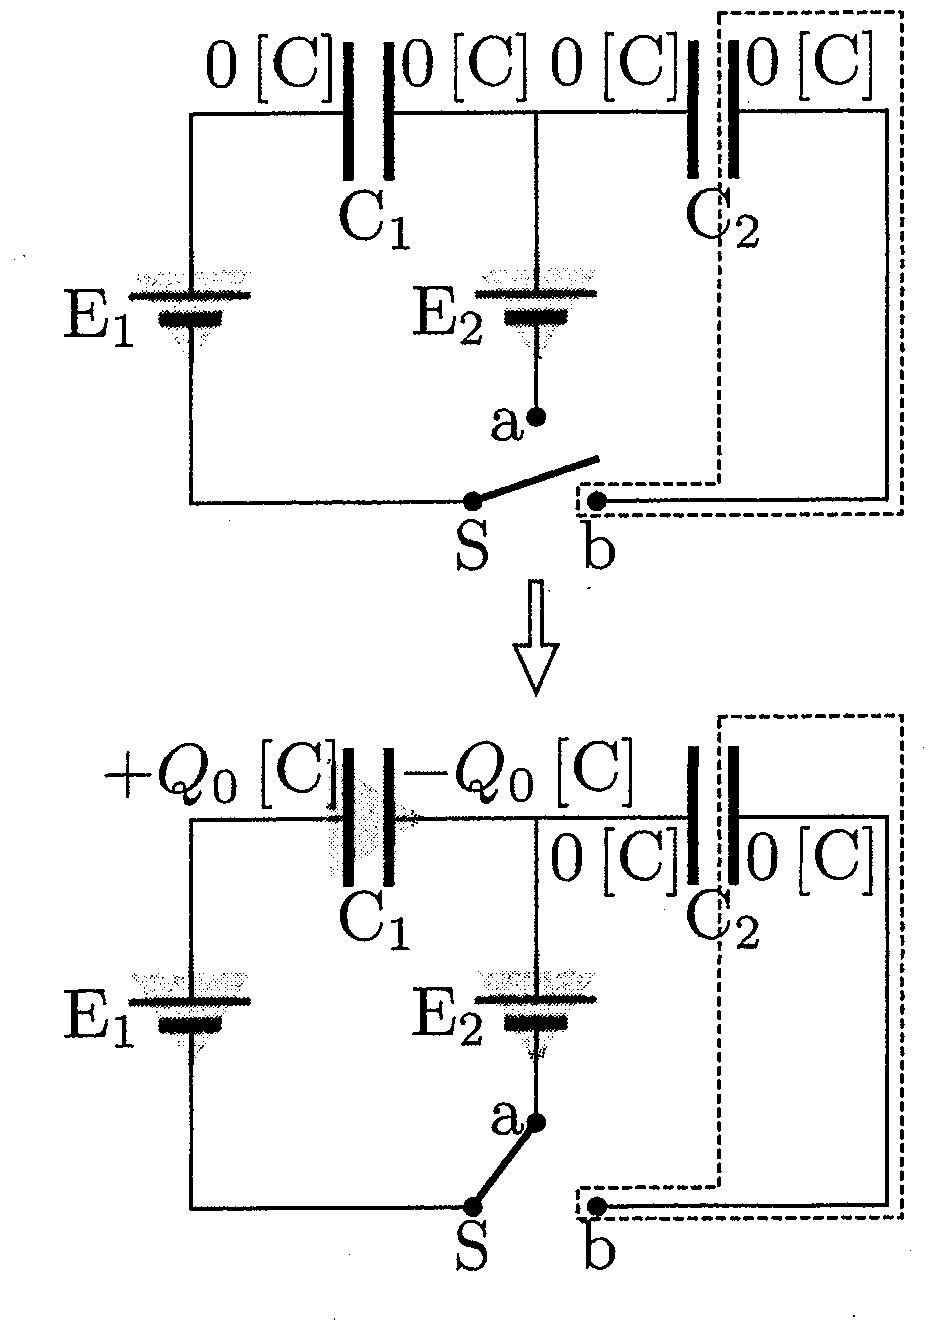
\includegraphics[keepaspectratio,width=58mm]{fig/n25_a52_zu1.png}\end{center}
       このとき，閉ループを作っているのは左側の部分だけであり，このループに対してキルヒホッフの第二法則を用いると（$\mathrm{a}$点を起点として時計回りに式を立てると），
       \[V-\frac{1}{2}V=\frac{Q_0}{2C}\]
       である．よってこれを解いて，
       \[Q_0=CV\U{C}\Ans\]
       またこのとき，$\mathrm{C}_1$に蓄えられている静電エネルギーは，
       \[U_0=\frac{1}{2}\cdot\frac{Q_0^2}{2C}=\frac{1}{4}CV^2\U{J}\Ans\]
\ko{2} $\mathrm{S}$を$\mathrm{a}$からいったん離したとき，電荷は移動しないので，$\mathrm{S}$を$\mathrm{a}$から離した状態での帯電状態は次図のようになる．
       \begin{center}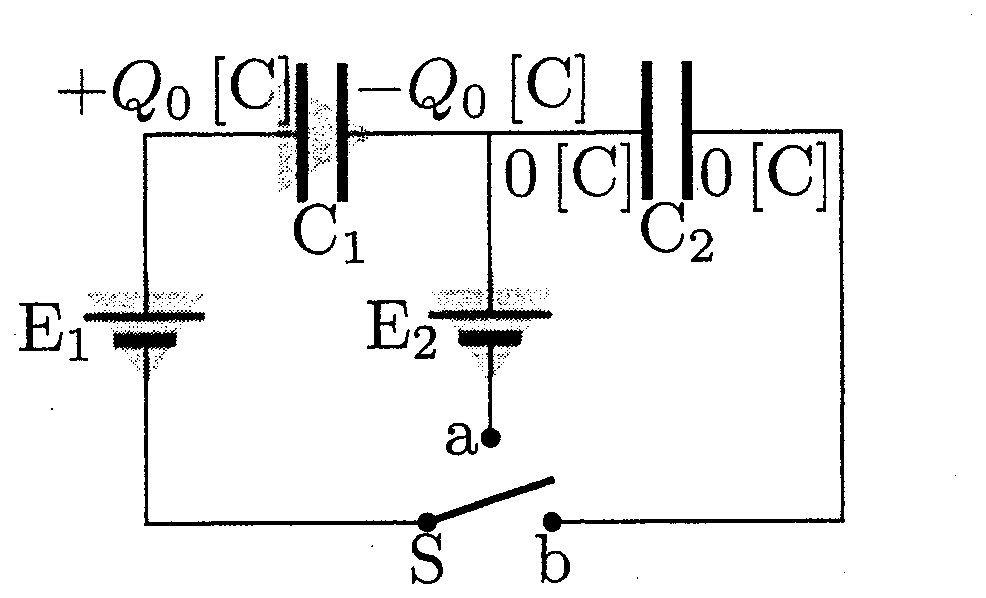
\includegraphics[keepaspectratio,width=56mm]{fig/n25_a52_zu2.png}\end{center}
       この状態からスイッチ$\mathrm{S}$を$\mathrm{b}$につなぐと，コンデンサー$\mathrm{C}_2$に対して電圧がかかるため，電荷が移動して新しい電荷分布となる．各コンデンサーの左側極板に帯電する電気量をそれぞれ$+Q_1\U{C}$，$+Q_2\U{C}$とおくと（どちらに正電荷が溜まるのかはっきりしないので適当に仮定した），スイッチ操作前後の帯電状態は次図のように変化する．
       \begin{center}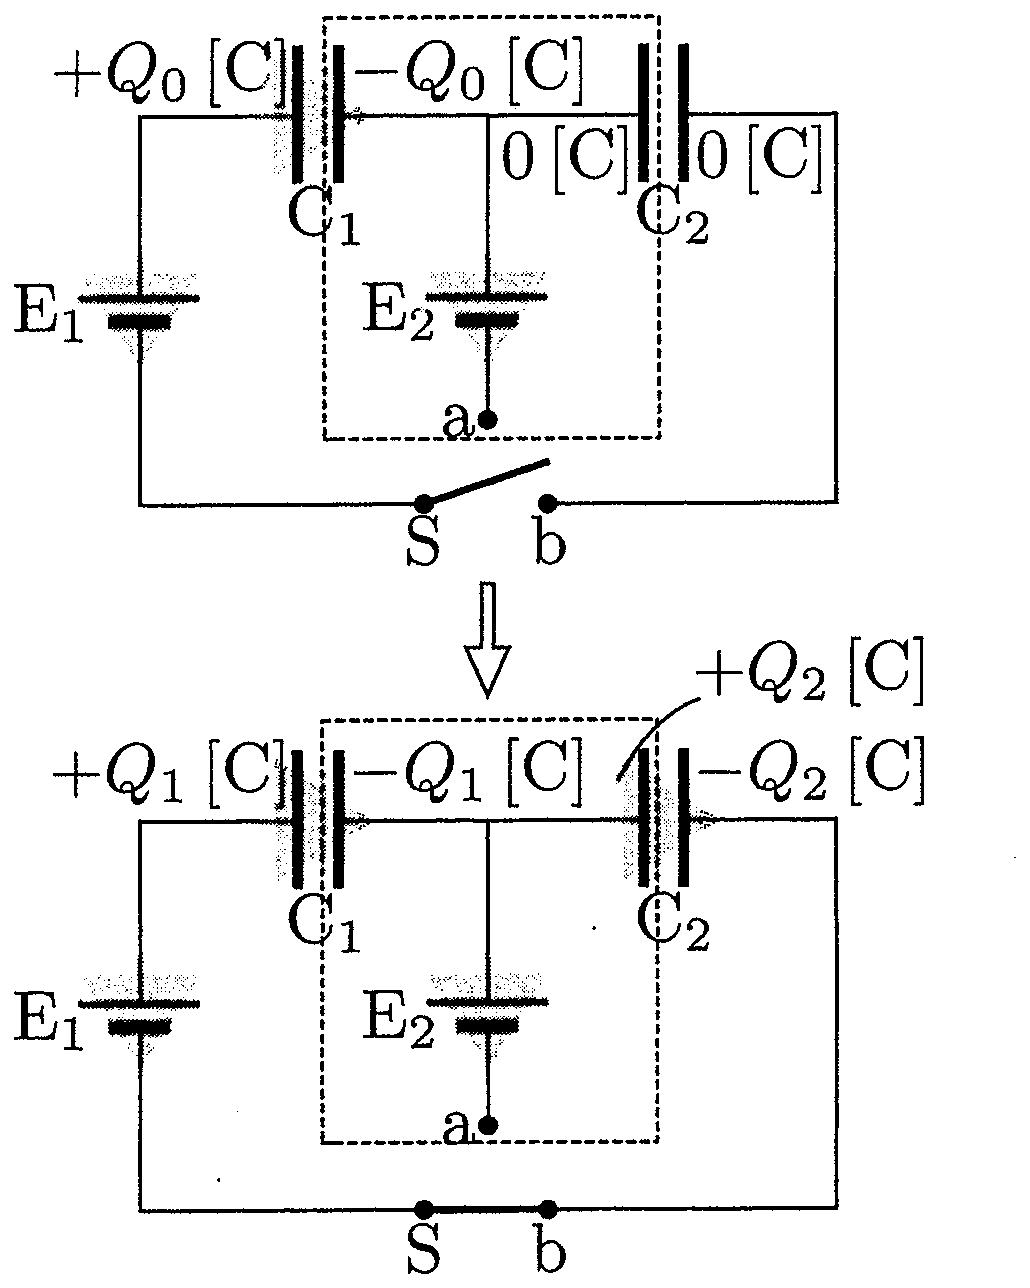
\includegraphics[keepaspectratio,width=56mm]{fig/n25_a52_zu3.png}\end{center}
       このとき，閉ループを作っているのは外周の部分だけであり，このループに対してキルヒホッフの第二法則を用いると，
       \[V=\frac{Q_1}{2C}+\frac{Q_2}{C}\]
       である．また，図の点線の四角枠囲み部分に着目すると，ここはスイッチ操作前後について，回路の他の部分と接続していない．よって，この部分に対して電荷保存の法則を適用すると，
       \[-Q_0+0=-Q_1+Q_2\]
       である．以上2式および(1)の答えを用いて計算すると，
       \[Q_1=\frac{4}{3}CV\U{C},\quad Q_2=\frac{1}{3}CV\U{C}\Ans\]
       \begin{chuu}
       出てきた答えの$Q_1$，$Q_2\U{C}$が確かに正であったので，仮定した電荷の正負の向きは正しかったことになる．

       また，上図では電池$\mathrm{E}_2$を含んだ点線枠内に対して電荷保存の法則を適用しているが，電荷保存の法則は枠内に電池を含んでいても構わない．なぜなら，電荷は枠内から出られないからである．ただし，コンデンサーと同じつもりで次図のように電池の二本線の間に点線を引いたりしないように！　記号では正極と負極は離れているが，電池はコンデンサーとは違い，正極と負極は電池内部で電気回路的につながっている．
       \begin{center}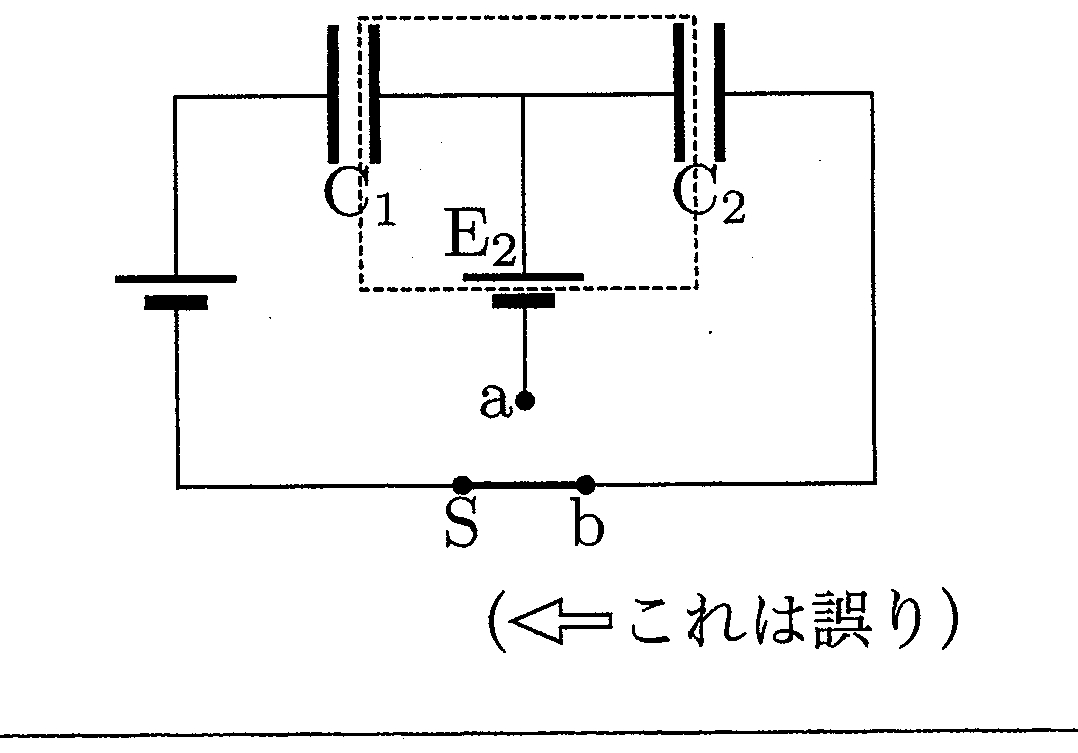
\includegraphics[keepaspectratio,width=52mm]{fig/n25_a52_zu4.png}\end{center}
       \end{chuu}
\ko{3} (2)の終状態での静電エネルギーの総和は，
       \[U_1=\frac{1}{2}\cdot\frac{Q_1^2}{2C}+\frac{1}{2}\cdot\frac{Q_2^2}{C}=\frac{1}{2}CV^2\U{J}\]
       であるから，全体の静電エネルギーの変化量は，
       \[U_1-\left(U_0+\frac{1}{2}\cdot\frac{0^2}{C}\right)=\frac{1}{4}CV^2\U{J}\Ans\]
       \begin{bsHosoku}{参考}
       (3)の結果より，静電エネルギーは増加しているが，これは電池を通って$\mathrm{C}_2$の右側極板から$\mathrm{C}_1$の左側極板に電荷が移動しているからである．電池$\mathrm{E}_1$を通過した電気量は
       \[Q_1-Q_0=\frac{1}{3}CV\U{C}\]
       であるから，電池は
       \[\frac{1}{3}CV\cdot V=\frac{1}{3}CV^2\U{J}\]
       の仕事をしている．よって，導線の持つわずかな抵抗から散逸した熱エネルギーは，電池がした仕事から静電エネルギーの増加に利用された分を差し引いて，
       \[\frac{1}{3}CV^2-\frac{1}{4}CV^2=\frac{1}{12}CV^2\U{J}\]
       になる．
       \end{bsHosoku}
\end{komon}

\MonN{53}{コンデンサーの連結}\par\nopagebreak
\begin{sisin}
考え方は前問と全く同様である．本問の場合はコンデンサーの合成（25.5）を利用しても考えられるが，前問と同様の方法で解いてみよう．
\end{sisin}
\KaiHead
\begin{komon}
\ko{1} スイッチの操作前後の回路図は下の通りである．左側を正として各極板の帯電量を次図のように仮定する．
       \begin{center}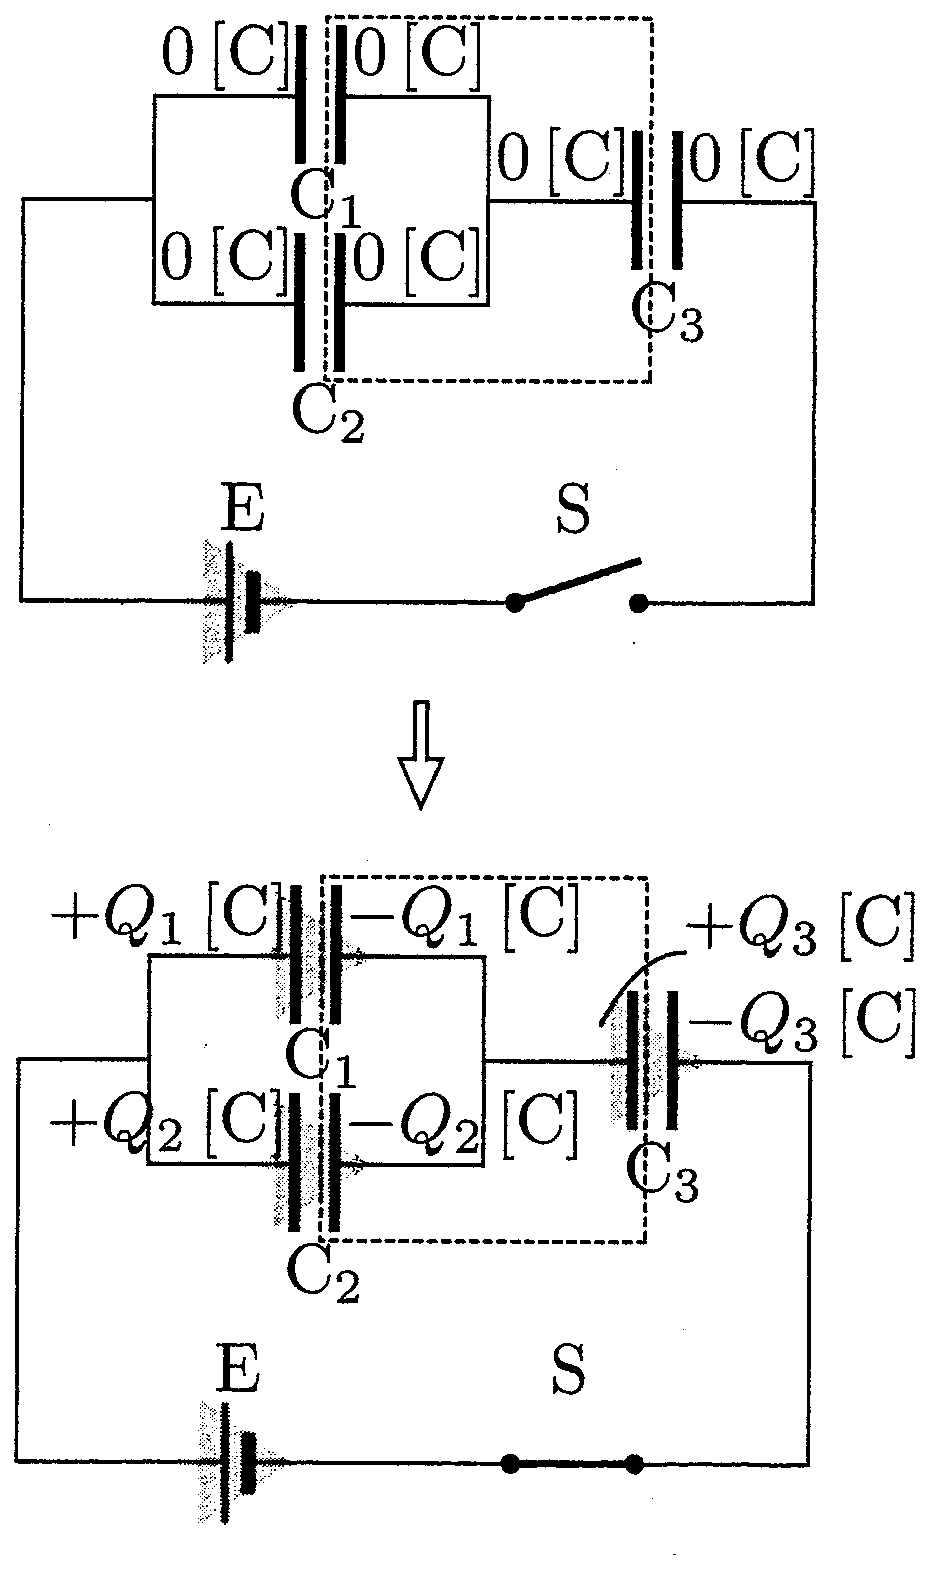
\includegraphics[keepaspectratio,width=56mm]{fig/n25_a53_zu.png}\end{center}
       このとき閉ループを作っているのは，\MARU{1}上側のコンデンサー$\mathrm{C}_1$，$\mathrm{C}_2$の部分のループと，\MARU{2}下側の，コンデンサー$\mathrm{C}_2$，$\mathrm{C}_3$，スイッチ$\mathrm{S}$，電池$\mathrm{E}$を含むループの二つであるから，これらのループに対してキルヒホッフの第二法則を用いると（時計回りに式を立てると），
       \[0=-\frac{Q_1}{2C}+\frac{Q_2}{3C},\quad V=\frac{Q_2}{3C}+\frac{Q_3}{5C}\]
       である．また，図の点線の四角枠囲み部分に着目すると，ここはスイッチ操作前後について，回路の他の部分と接続していない．よって，この部分に対して電荷保存の法則を適用すると，
       \[0+0+0=-Q_1-Q_2+Q_3\]
       である．以上3式を整理・計算すると，
       \[Q_1=CV\U{C},\quad Q_2=\frac{3}{2}CV\U{C}\]
       \[Q_3=\frac{5}{2}CV\U{C}\Ans\]
       \begin{chuu}
       上述の解答では，\MARU{1}と\MARU{2}のループについてキルヒホッフの第二法則を用いたが，これ以外に，\MARU{3}外周の，コンデンサー$\mathrm{C}_1$，$\mathrm{C}_3$，スイッチ$\mathrm{S}$，電池$\mathrm{E}$を含むループも考えることができる．これに対してキルヒホッフの第二法則を用いると，
       \[V=\frac{Q_1}{2C}+\frac{Q_3}{5C}\]
       という式を立てることができるが，この式は\MARU{1}と\MARU{2}のキルヒホッフの第二法則の式の変形によって導くことができるため，\MARU{1}，\MARU{2}と数学的に独立な式ではない．そのため，本問のように回路上ではさまざまなループが考えられる場合であっても，\MARU{1}〜\MARU{3}のうち，数学的に意味のある式は二つしかない．
       \end{chuu}
\ko{2} このときの各極板間電位差は，
       \[V_1=\frac{Q_1}{2C}=\frac{1}{2}V\U{V},\quad V_2=\frac{Q_2}{3C}=\frac{1}{2}V\U{V}\]
       \[V_3=\frac{Q_3}{5C}=\frac{1}{2}V\U{V}\Ans\]
\end{komon}

\MonN[\Sitei]{54}{コンデンサー回路のスイッチ操作}\par\nopagebreak
\begin{sisin}
スイッチの複数回切り替えの問題であるが，やはり解き方は前問までと全く同じである．本問のように多数回切り替えの場合には文字がこんがらがってくる危険性があるので，うまく文字を設定しながら考えていくとよい．

ただし，本問のようなスイッチの多数回の切り替え問題の場合は，電位を元に考えていくと容易に解ける場合があり，本問の場合は電位を元に各極板の帯電量を考えるとあっさりと解ける．これについては別解として示す．

なお，本問で利用している検流計とは通過した電気量を測る装置であるが，電荷が移動しなくなったとき（電流が流れていないとき）には検流計には電圧がかからないので，キルヒホッフの第二法則を用いる際にはただの導線と同様にして扱えばよい（25.6）．
\end{sisin}
\KaiHead
\begin{komon}
\ko{1} $\mathrm{K}_1$のみを閉じたとき，$\mathrm{C}_3$の右側極板には電荷が流入しないので，$\mathrm{C}_3$の帯電量は$0$のままである（右下点線枠内の電荷保存則より）．$\mathrm{C}_1$，$\mathrm{C}_2$の帯電量を図のように$Q_1$，$Q_2\U{C}$とする．
       \begin{center}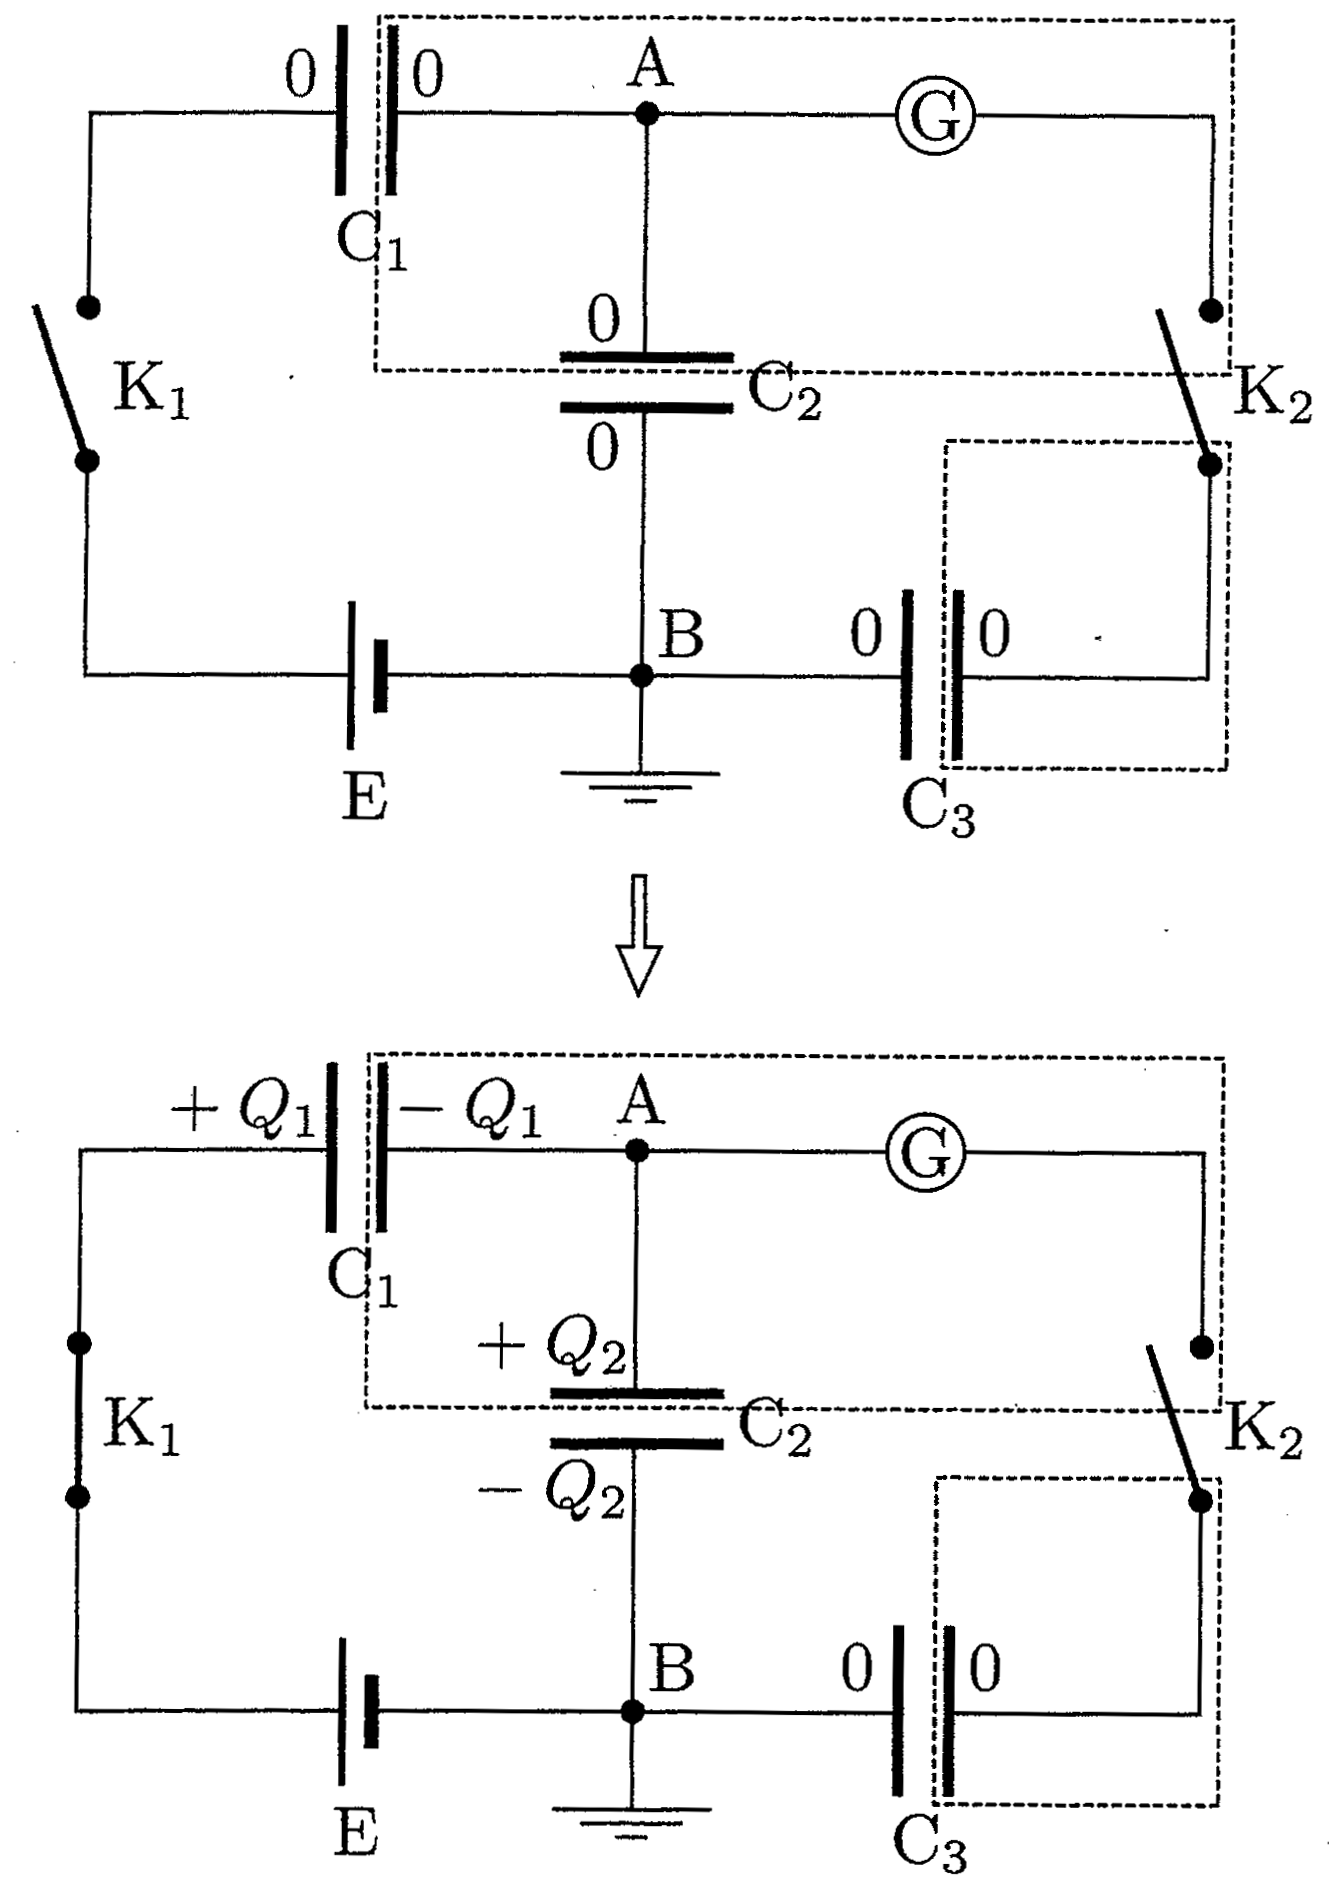
\includegraphics[keepaspectratio,width=64mm]{fig/n25_a54_zu1.png}\end{center}
       このとき，上の枠内の電荷保存則およびキルヒホッフの第二法則より，
       \[0=-Q_1+Q_2,\quad E=\frac{Q_1}{C}+\frac{Q_2}{2C}\]
       であるから，これらを解いて，
       \[Q_1=Q_2=\frac{2}{3}CE\U{C}\]
       よって，$\mathrm{A}$点の電位は
       \[\frac{Q_2}{2C}=\frac{1}{3}E\U{V}\Ans\]
\ko{2} $\mathrm{K}_1$を開いてから$\mathrm{K}_2$を閉じる．このとき，左上の部分は回路の他の部分と接触がないので，$\mathrm{C}_1$の左側極板の帯電量$+\dfrac{2}{3}CE\U{C}$はそのまま保たれる．また，コンデンサーは必ず向かい合う極板に正負逆，同じ大きさの電荷が帯電するので，$\mathrm{C}_1$の右側極板の帯電量は$-\dfrac{2}{3}CE\U{C}$のまま変化しないことになる．

       $\mathrm{C}_2$，$\mathrm{C}_3$の帯電量は変化しうるので，その帯電量を図のように$Q_2^\prime$，$Q_3^\prime\U{C}$とする．
       \begin{center}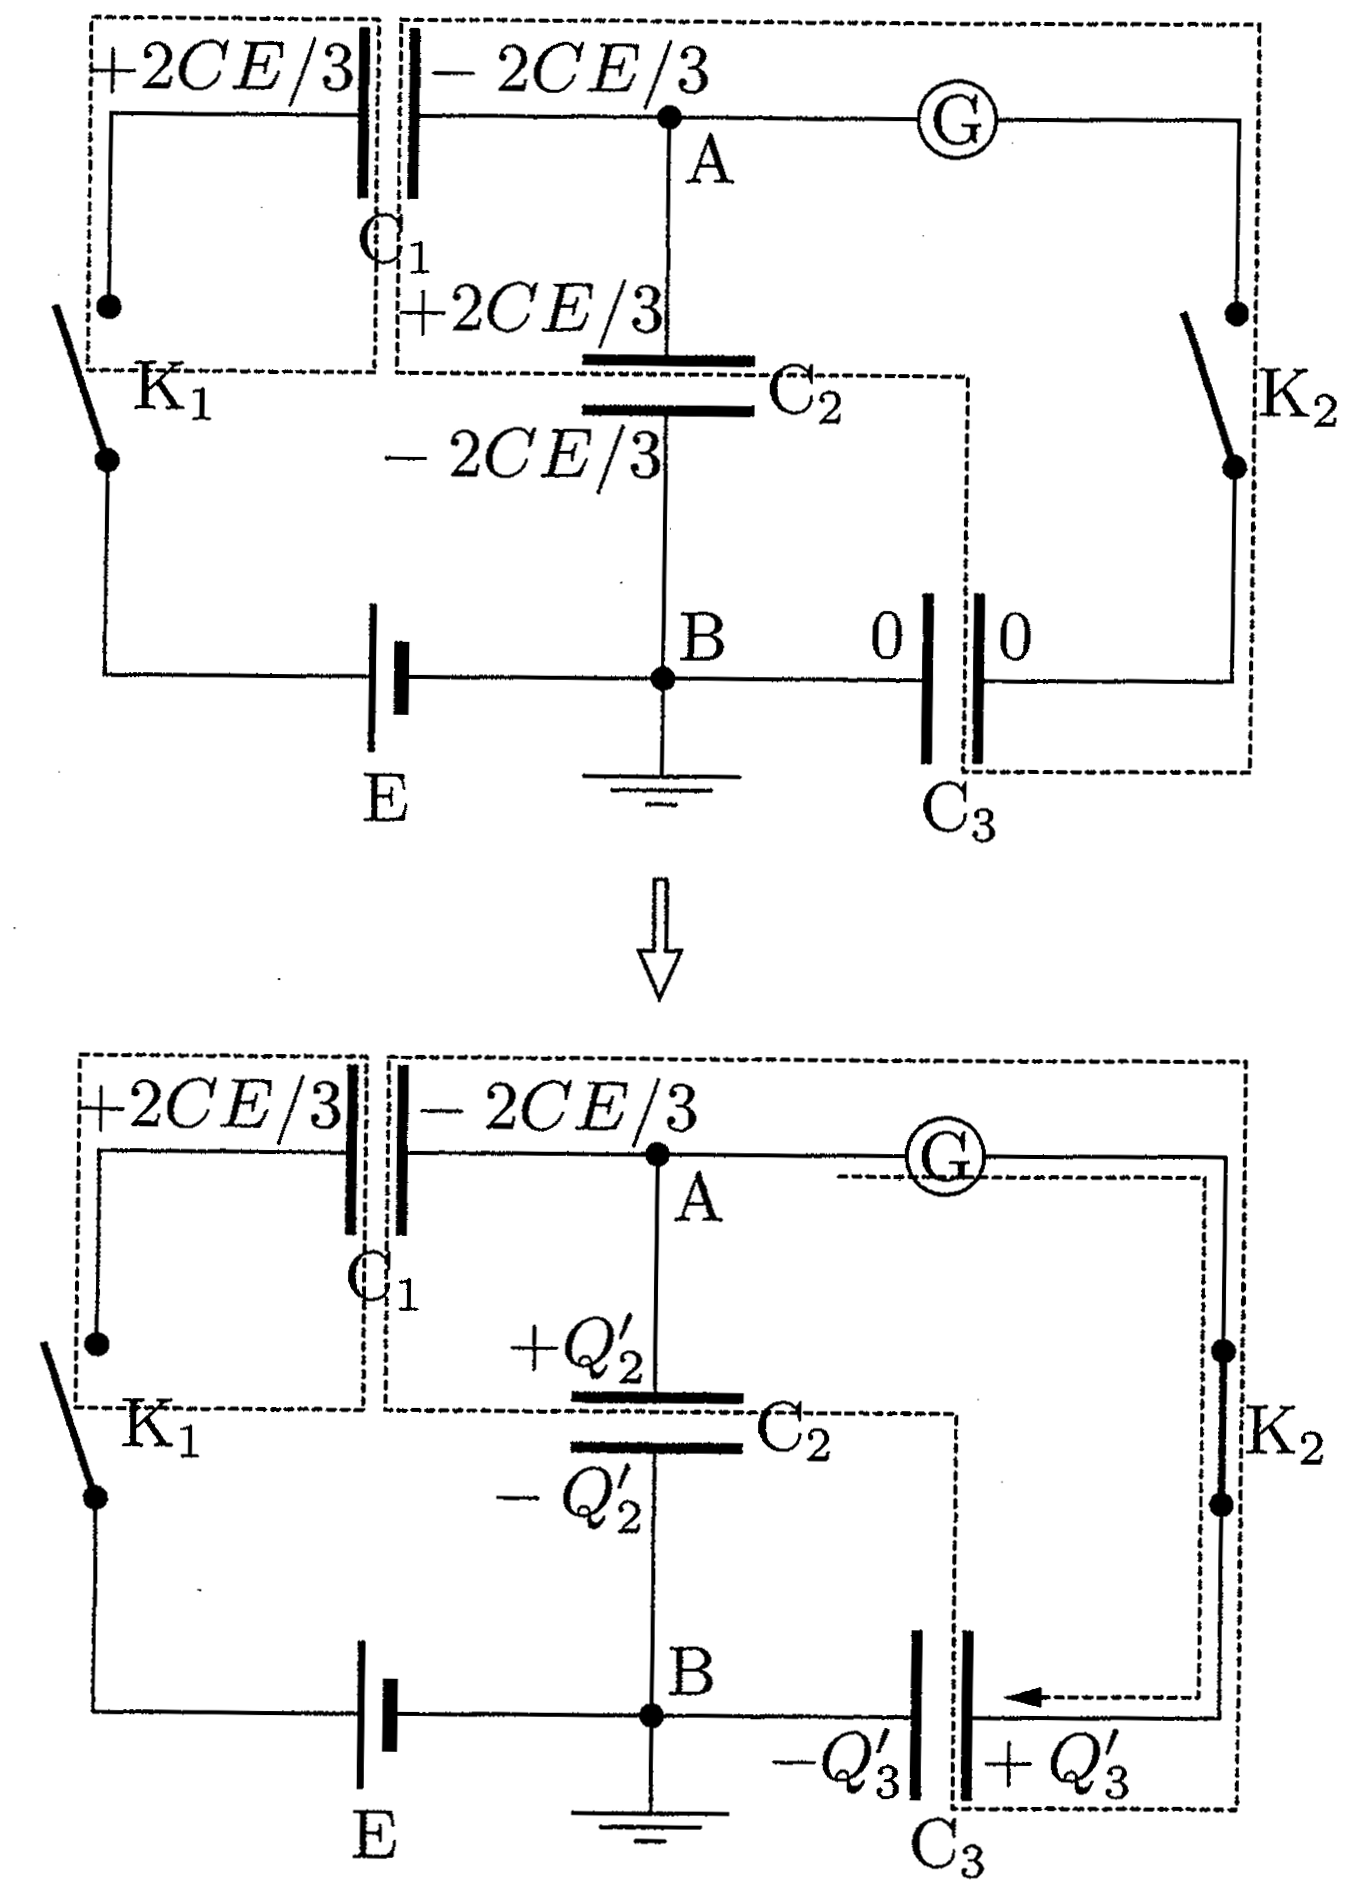
\includegraphics[keepaspectratio,width=64mm]{fig/n25_a54_zu2.png}\end{center}
       このとき，右側の枠内の電荷保存則およびキルヒホッフの第二法則より，
       \[-\frac{2}{3}CE+\frac{2}{3}CE+0=-\frac{2}{3}CE+Q_2^\prime+Q_3^\prime\]
       \[0=\frac{Q_2^\prime}{2C}-\frac{Q_3^\prime}{3C}\]
       であるから，これらを解いて，
       \[Q_2^\prime=\frac{4}{15}CE\U{C},\quad Q_3^\prime=\frac{2}{5}CE\U{C}\]
       である．よって，このときの$\mathrm{A}$点の電位は
       \[\frac{Q_2^\prime}{2C}=\frac{2}{15}E\U{V}\Ans\]
\ko{3} 検流計$\mathrm{G}$を通過した電荷は，上図に示したように$\mathrm{C}_3$の右側極板に蓄積されるので，$\mathrm{C}_3$の右側極板の電荷の増加量が検流計$\mathrm{G}$を右向きに通過した電荷である．よって，
       \[Q_3^\prime-0=\frac{2}{5}CE\U{C}\Ans\]
\ko{4} $\mathrm{K}_2$を開いてから$\mathrm{K}_1$を閉じる．このとき，右下の部分は回路の他の部分と接触がないので，$\mathrm{C}_3$の右側極板の帯電量$+\dfrac{2}{5}CE\U{C}$はそのまま保たれる．また，コンデンサーは必ず向かい合う極板に正負逆，同じ大きさの電荷が帯電するので，$\mathrm{C}_3$の左側極板の帯電量は$-\dfrac{2}{5}CE\U{C}$のまま変化しないことになる．$\mathrm{C}_1$，$\mathrm{C}_2$の帯電量を図のように$Q_1^{\prime\prime}$，$Q_2^{\prime\prime}\U{C}$とする．
       \begin{center}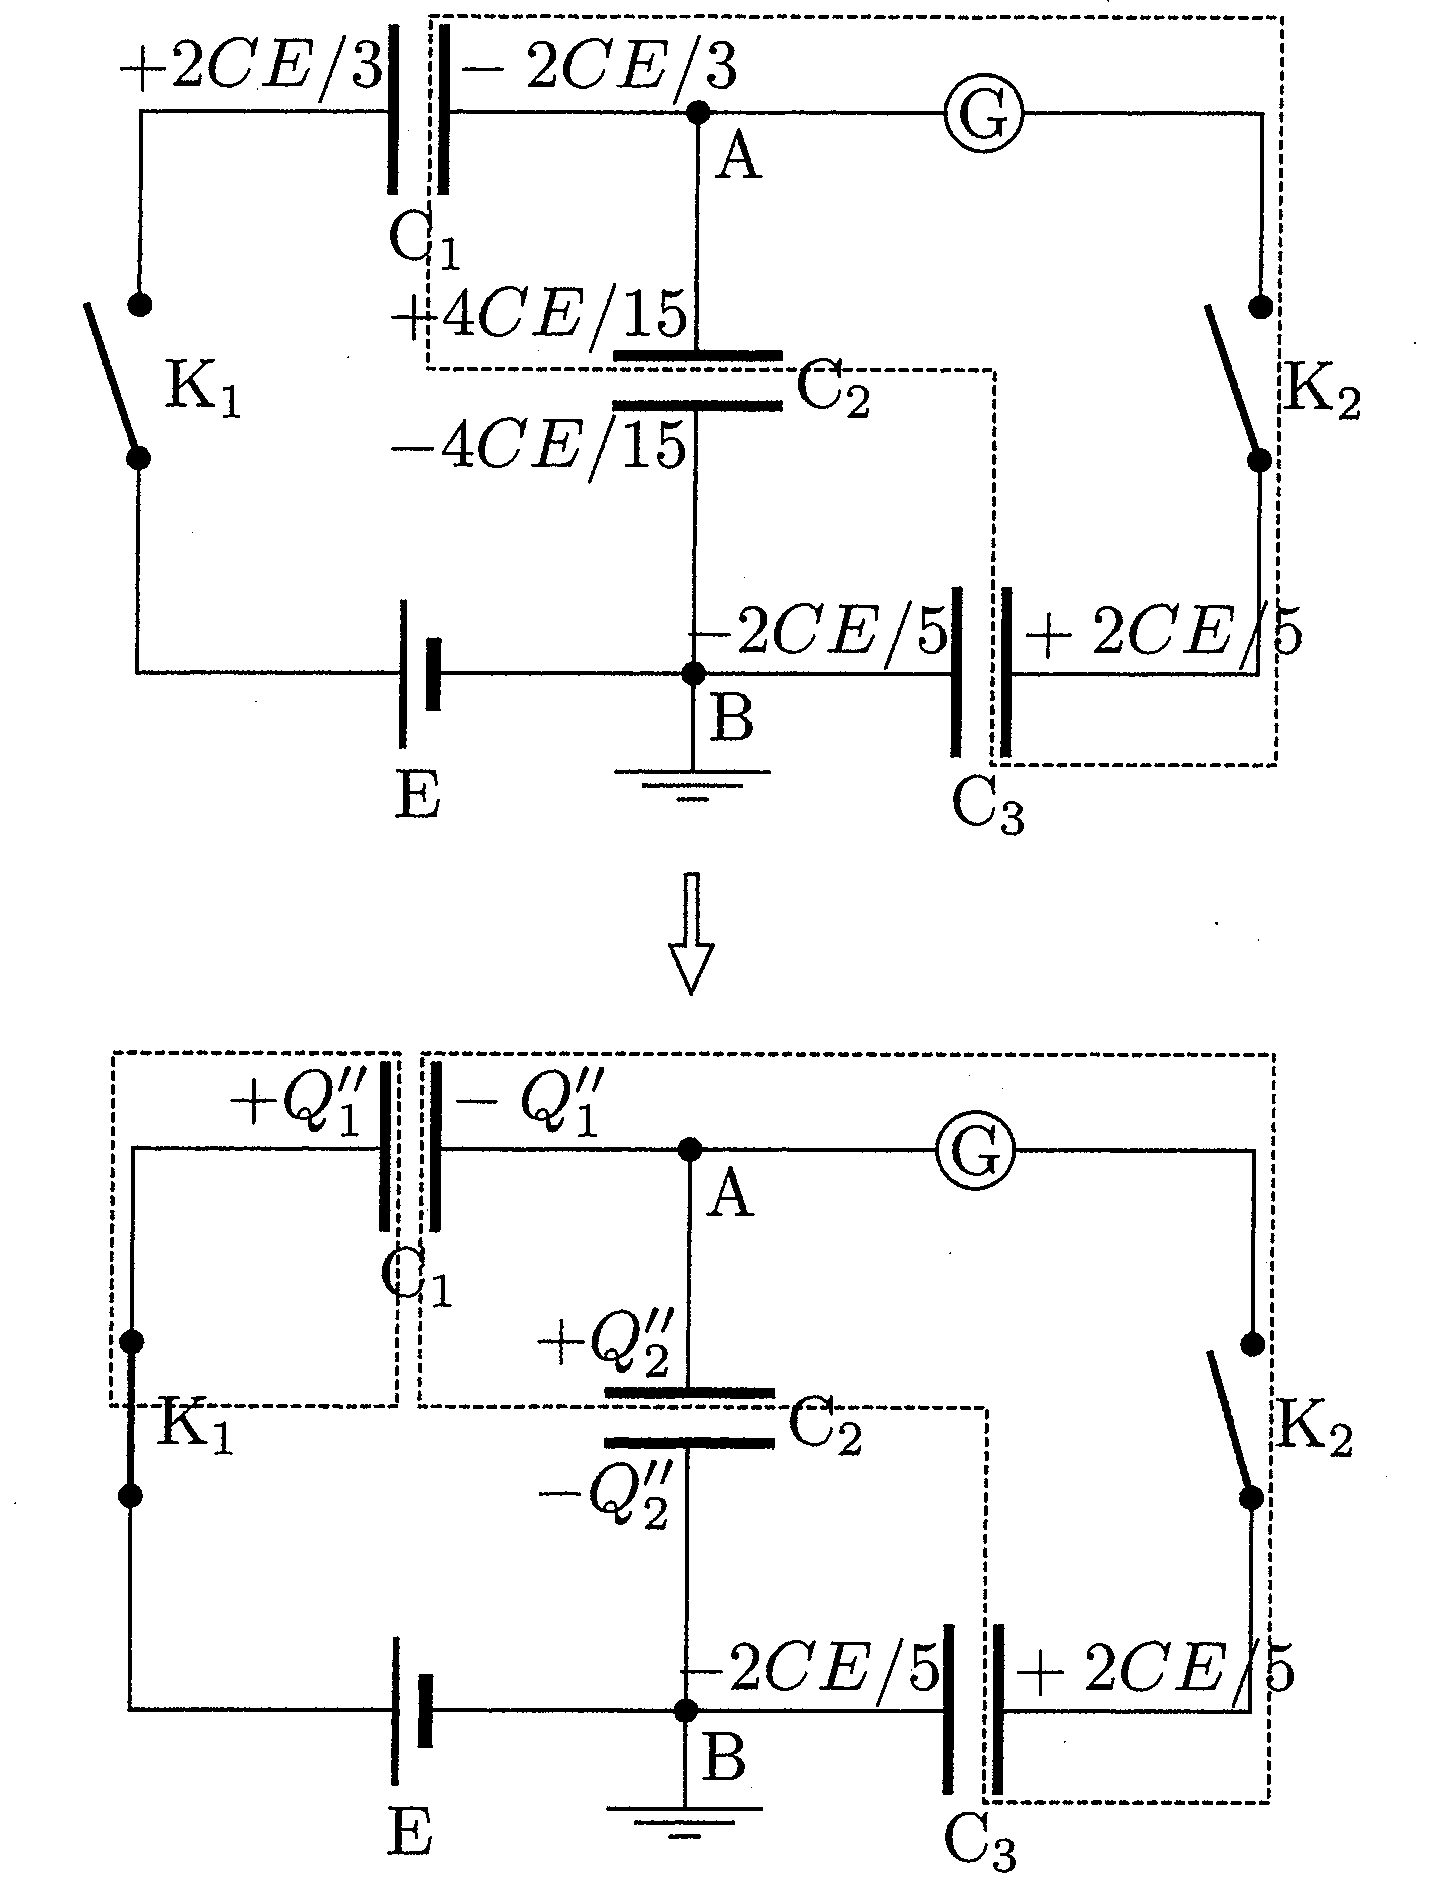
\includegraphics[keepaspectratio,width=64mm]{fig/n25_a54_zu3.png}\end{center}
       このとき，上の枠内の電荷保存則およびキルヒホッフの第二法則より，
       \[-\frac{2}{3}CE+\frac{4}{15}CE=-Q_1^{\prime\prime}+Q_2^{\prime\prime}\]
       \[E=\frac{Q_1^{\prime\prime}}{C}+\frac{Q_2^{\prime\prime}}{2C}\]
       であるから，これらを解いて，
       \[Q_1^{\prime\prime}=\frac{4}{5}CE\U{C},\quad Q_2^{\prime\prime}=\frac{2}{5}CE\U{C}\]
       よって，$\mathrm{A}$点の電位は
       \[\frac{Q_2^{\prime\prime}}{2C}=\frac{1}{5}E\U{V}\Ans\]
\end{komon}
\begin{bekkai}
指針で述べた，電位を用いて考える方法を以下に示す．本問の場合には，$\mathrm{A}$点の電位$V_{\mathrm{A}}\U{V}$が決まるとすべての極板上の電荷が$V_{\mathrm{A}}\U{V}$を用いて表せるので，電荷保存則のみを考えればよく，非常に簡単に問題を解くことができる．この解法を以下に示す（番号は設問の番号に合わせた）．
\begin{komon}
\ko{1} $\mathrm{K}_1$のみを閉じたときの$\mathrm{A}$点の電位を$V_{\mathrm{A}}\U{V}$とする．まず，$\mathrm{C}_3$の右側極板には電荷が流入しないので，$\mathrm{C}_3$の帯電量は$0$のままである．コンデンサー$\mathrm{C}_2$の下側極板の電位は$0\U{V}$，上側極板の電位は$V_{\mathrm{A}}\U{V}$ゆえ，$\mathrm{C}_2$にかかる電圧は$V_{\mathrm{A}}-0=V_{\mathrm{A}}\U{V}$である．よって，$\mathrm{C}_2$の上側極板の電荷は$+2CV_{\mathrm{A}}\U{C}$，下側極板の電荷は$-2CV_{\mathrm{A}}\U{C}$である．

       コンデンサー$\mathrm{C}_1$については，左側極板の電位が$E\U{V}$，右側極板の電位が$V_{\mathrm{A}}\U{V}$であるから，$\mathrm{C}_1$にかかる電圧は$E-V_{\mathrm{A}}\U{V}$である．よって，$\mathrm{C}_1$の左側極板の電荷は$+C(E-V_{\mathrm{A}})\U{C}$，右側極板の電荷は$-C(E-V_{\mathrm{A}})\U{C}$である．

       ここで，上の解答の点線枠内の電荷保存則を考えることにより，
       \[0=-C(E-V_{\mathrm{A}})+2CV_{\mathrm{A}}\]
       であるから，これを解いて，
       \[V_{\mathrm{A}}=\frac{1}{3}E\U{V}\Ans\]
\ko{2} $\mathrm{K}_1$を開いてから$\mathrm{K}_2$を閉じたとき，左上の部分は回路の他の部分と接触がないので，$\mathrm{C}_1$の左側極板の帯電量$+\dfrac{2}{3}CE\U{C}$はそのまま保たれる．また，コンデンサーは必ず向かい合う極板に正負逆，同じ大きさの電荷が帯電するので，$\mathrm{C}_1$の右側極板の帯電量は$-\dfrac{2}{3}CE\U{C}$のまま変化しない．このときの$\mathrm{A}$点の電位を$V_{\mathrm{A}}^\prime\U{V}$とすると，前問と同様な考えにより，$\mathrm{C}_2$の上側極板の電荷は$+2CV_{\mathrm{A}}^\prime\U{C}$，下側極板の電荷は$-2CV_{\mathrm{A}}^\prime\U{C}$，$\mathrm{C}_3$の右側極板の電荷は$+3CV_{\mathrm{A}}^\prime\U{C}$，左側極板の電荷は$-3CV_{\mathrm{A}}^\prime\U{C}$である．

       ここで，上の解答の点線枠内の電荷保存則を考えることにより，
       \[\begin{aligned}
         &-\frac{2}{3}CE+\frac{2}{3}CE+0\\
         &\qquad=-\frac{2}{3}CE+2CV_{\mathrm{A}}^\prime+3CV_{\mathrm{A}}^\prime
       \end{aligned}\]
       であるから，これを解くと，
       \[V_{\mathrm{A}}^\prime=\frac{2}{15}E\U{V}\Ans\]
\ko{4} $\mathrm{K}_2$を開いてから$\mathrm{K}_1$を閉じる．このとき，右下の部分は回路の他の部分と接触がないので，$\mathrm{C}_3$の右側極板の帯電量$+\dfrac{2}{5}CE\U{C}$はそのまま保たれる．また，コンデンサーは必ず向かい合う極板に正負逆，同じ大きさの電荷が帯電するので，$\mathrm{C}_3$の左側極板の帯電量は$-\dfrac{2}{5}CE\U{C}$のまま変化しないことになる．このときの$\mathrm{A}$点の電位を$V_{\mathrm{A}}^{\prime\prime}\U{V}$とすると，(1)と同様な考えにより，$\mathrm{C}_2$の上側極板の電荷は$+2CV_{\mathrm{A}}^{\prime\prime}\U{C}$，下側極板の電荷は$-2CV_{\mathrm{A}}^{\prime\prime}\U{C}$，$\mathrm{C}_1$の左側極板の電荷は$+C(E-V_{\mathrm{A}}^{\prime\prime})\U{C}$，右側極板の電荷は$-C(E-V_{\mathrm{A}}^{\prime\prime})\U{C}$である．

       ここで，上の解答の点線枠内の電荷保存則を考えると，
       \[\begin{aligned}
         &-\frac{2}{3}CE+\frac{4}{15}CE\\
         &\qquad=-C(E-V_{\mathrm{A}}^{\prime\prime})+2CV_{\mathrm{A}}^{\prime\prime}
       \end{aligned}\]
       であるから，これを解いて，
       \[V_{\mathrm{A}}^{\prime\prime}=\frac{1}{5}E\U{V}\Ans\]
\end{komon}
この別解の方法では，$\mathrm{A}$点の電位を元に各コンデンサーの帯電量を求めているが，これを行えば自動的に回路のキルヒホッフの第二法則は満足される．よって，電荷保存則のみを考えればよくなり，容易に問題を解くことができる．

ただし，この解法を用いることができるのは，ある一点の電位によりすべての極板上の電荷が容易に表現できるような系に限られる．そうでない場合にはオーソドックスに極板上の電荷を仮定し，電荷保存則・キルヒホッフの第二法則を組み合わせて考えるしかない．
\end{bekkai}

% ［55］は原本の【例題13】（再編案で例題→練習へ格下げ）．原本は例題なので解答が
%   載っていない（指針だけ）．解答は書き起こした．
\MonN{55}{複合極板コンデンサー}\par\nopagebreak
\begin{sisin}
複雑なコンデンサーは単純なコンデンサーの合成だとみなして回路を書き換え，コンデンサー回路の考え方（25.6）に従って電荷分布を求める．書き換えの4つの型は25.7にまとめてある．

なお本問は，どの場合も電池がつながれたままなので極板間の電圧は$V\U{V}$で変わらない．したがって合成容量さえ求まれば$Q=CV$で答えが出る．
\end{sisin}
\KaiHead
極板面積を$S\U{m^2}$，極板間隔を$d\U{m}$，真空の誘電率を$\varepsilon_0\U{C^2/N\cdot m^2}$とすると，もとのコンデンサーの電気容量は$C=\varepsilon_0\dfrac{S}{d}\U{F}$である．
\begin{komon}
\ko{1} 金属板の部分は導線とみなせるので，このコンデンサーは極板間隔$\dfrac{d}{4}\U{m}$のコンデンサー2つの直列接続になる（金属板の厚さが$\dfrac{d}{2}$なので，残ったすき間$\dfrac{d}{2}$が上下に二等分される）．それぞれの電気容量は
       \[\varepsilon_0\frac{S}{d/4}=4C\U{F}\]
       であるから，合成容量$C^\prime$は
       \[\frac{1}{C^\prime}=\frac{1}{4C}+\frac{1}{4C}\quad\text{より}\quad C^\prime=2C\U{F}\]
       よって，蓄えられる電気量は
       \[Q=C^\prime V=2CV\U{C}\Ans\]
\ko{2} 左半分（真空）と右半分（誘電体）の並列接続とみなせる．極板面積がそれぞれ$\dfrac{S}{2}$になるので，
       \[C_1=\varepsilon_0\frac{S/2}{d}=\frac{1}{2}C\U{F}\]
       \[C_2=\varepsilon_{\mathrm{r}}\varepsilon_0\frac{S/2}{d}=\frac{\varepsilon_{\mathrm{r}}}{2}C\U{F}\]
       であり，合成容量は$C^\prime=C_1+C_2=\dfrac{1+\varepsilon_{\mathrm{r}}}{2}C\U{F}$．よって，
       \[Q=C^\prime V=\frac{1+\varepsilon_{\mathrm{r}}}{2}CV\U{C}\Ans\]
\ko{3} 金属板は厚さが無視でき，帯電もしていないので，上半分（真空・間隔$\dfrac{d}{2}$）と下半分（誘電体・間隔$\dfrac{d}{2}$）の直列接続とみなせる．
       \[\begin{aligned}
         &C_1=\varepsilon_0\frac{S}{d/2}=2C\U{F}\\
         &C_2=\varepsilon_{\mathrm{r}}\varepsilon_0\frac{S}{d/2}=2\varepsilon_{\mathrm{r}}C\U{F}
       \end{aligned}\]
       であるから，
       \[\frac{1}{C^\prime}=\frac{1}{2C}+\frac{1}{2\varepsilon_{\mathrm{r}}C}=\frac{1+\varepsilon_{\mathrm{r}}}{2\varepsilon_{\mathrm{r}}C}\]
       より$C^\prime=\dfrac{2\varepsilon_{\mathrm{r}}}{1+\varepsilon_{\mathrm{r}}}C\U{F}$．よって，
       \[Q=C^\prime V=\frac{2\varepsilon_{\mathrm{r}}}{1+\varepsilon_{\mathrm{r}}}CV\U{C}\Ans\]
       \begin{chuu}
       (3)で挿入した金属板は，厚さが無視でき帯電もしていないので，結果には全く影響しない．{\gtfamily 帯電していない厚さ0の金属板は，入れても入れなくても同じ}である．
       \end{chuu}
\end{komon}

\Rank{C問題}
\MonN{56}{導体球の電気容量}\par\nopagebreak
\begin{sisin}
金属（導体）の性質を整理しておくこと．\MARU{1}金属に帯電した電荷は表面のみに分布し，内部には分布しない．\MARU{2}金属内部の電場は$0$なので，金属内部および表面の電位は等しい．\MARU{3}金属表面は等電位面になるので，金属表面付近の電場は表面に対して垂直になる．

本問のような，導体球に対して電荷を与えた場合に作られる電場・電位は，その電荷が中心位置に集中した点電荷の場合と全く同様になる，ということは有名事実として覚えておくこと．
\end{sisin}
\KaiHead
\begin{komon}
\ko{1} 反発\Ans
\ko{2} 表面（導体内部では電荷は自由に動き回れるので，表面まで逃げて散乱して分布する）\Ans
\ko{3} 等電位\Ans
\ko{4} 垂直\Ans
\ko{5} 中心\Ans
\ko{6} $k\dfrac{Q}{r}\U{V}$\Ans
\ko{7} $k\dfrac{Q}{a}\U{V}$\Ans
\ko{8} \MARU{2}\Ans
\ko{9} $k\dfrac{Q}{a}\U{V}$（無限遠方の電位は$0\U{V}$であるから，これと(7)との電位差はこの値になる）\Ans
\ko{10} $\dfrac{a}{k}\U{F}$（$Q=CV$に当てはめると$Q=C\cdot k\dfrac{Q}{a}$であり，これを解く）\Ans
\end{komon}
\begin{bsHosoku}{参考}
問題文の誘導では直観的に，導体球の外側の電気力線の様子は，正電荷$Q\U{C}$が球の中心に点電荷として存在しているときに作られる電気力線の様子と全く同じであるとしているが，これを数学的に示すためにはガウスの法則を用いる必要がある．導体球の中心を中心とする半径$r\U{m}$の球面を考える．空間的に対称になっているので，電場はこの球面に対して垂直な向きであり，また問題文の考察より外向きである．
\begin{center}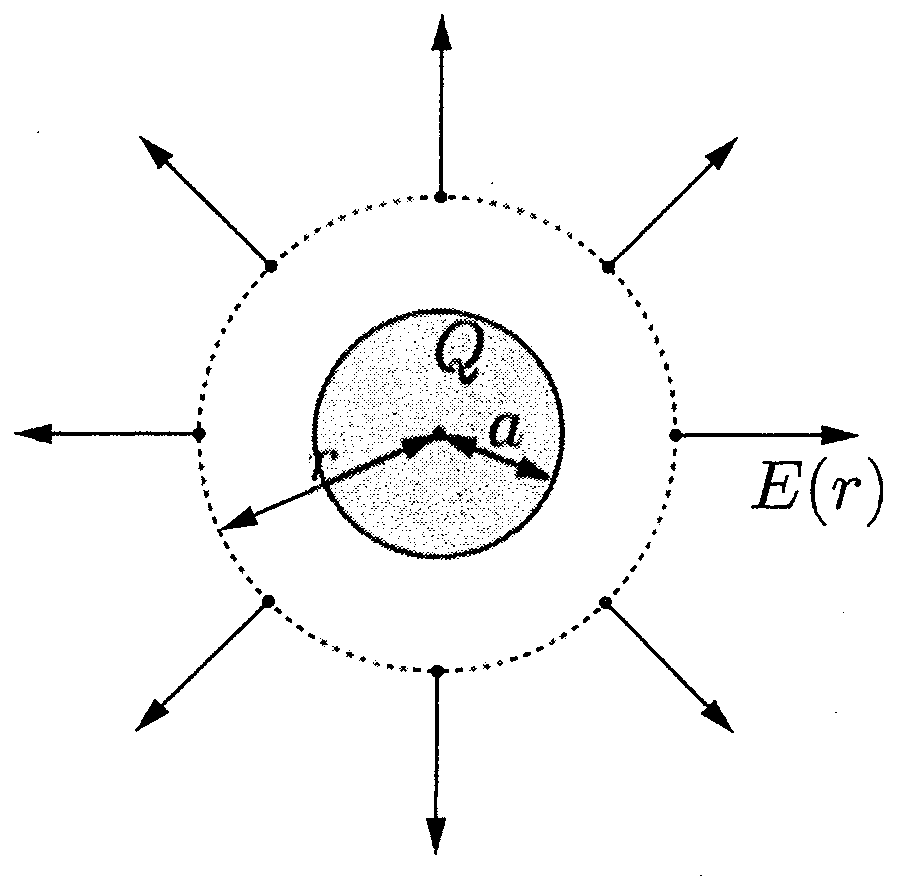
\includegraphics[keepaspectratio,width=52mm]{fig/n25_a56_zu.png}\end{center}
ここで，この半径$r\U{m}$の球面に対してガウスの法則を適用すると，球の表面積が$4\pi r^2\U{m^2}$であることに注意して，
\[4\pi r^2\cdot E(r)=4\pi k\cdot Q\]
である．これを解くと，
\[E(r)=k\frac{Q}{r^2}\U{V/m}\]
% 原本はここが $E(r)=kQ/r$ になっているが，左辺の $4\pi r^2 E(r)$ から明らかに
%   $kQ/r^2$ が正しい（誤植）．
となり，これは中心に点電荷$Q\U{C}$が存在する場合に作られる電場と全く同一である．電場が共通であれば電位も同じ表式になるので，電荷を持つ導体球が作る電場・電位は点電荷と同じように考えてよい，ということが言えるわけである．
\end{bsHosoku}

\MonN{57}{誘電体と誘電分極}\par\nopagebreak
\begin{sisin}
誘電体によって電場が弱められる様子を，定量的に考えようという問題である．25.3にあるように，間に挟み込んだ誘電体に電場をかけると誘電分極が生じ，結果として誘電体の極板付近の部分に，極板上の電荷を打ち消すような電荷（これを{\gtfamily 分極電荷}といい，図中の$\delta+$，$\delta-$がこれである）が発生する．この分極電荷をコンデンサーの電荷と同様にして扱う．

極板上の電荷から発生する電気力線（図中の太線）は，\underline{誘電体の}\hskip0pt\underline{有無によ}\hskip0pt\underline{って変化}\hskip0pt\underline{しない}．なぜなら，極板上の電荷からどう電気力線が出ていくかはガウスの法則によって決まるからであり，誘電体があろうとなかろうと$4\pi kQ$本の電気力線の出入りがある．

分極電荷に対してもこれと同様な扱い方をすることにより，図中の$\delta E$を求めよう．
\end{sisin}
\KaiHead
\begin{komon}
\ko{1} 自由電子（金属中の電子で，金属結合に寄与する，金属内を自由に動ける電子のことを自由電子という）\Ans
\ko{2}[\hspace{-1.9zw}\makebox[1.9zw][r]{(2)(3)}] コンデンサー$\mathrm{A}$，$\mathrm{B}$の電気容量はそれぞれ
       \[C_{\mathrm{A}}=\varepsilon_0\frac{S}{d}\U{F},\quad C_{\mathrm{B}}=\varepsilon_{\mathrm{r}}\varepsilon_0\frac{S}{d}\U{F}\]
       であり，これらに電圧$V\U{V}$の電池が接続されたので，蓄えられる電荷は，
       \[Q_{\mathrm{A}}=C_{\mathrm{A}}V=\frac{\varepsilon_0SV}{d}\U{C}\quad\cdots\cdots\text{(2)}\Ans\]
       \[Q_{\mathrm{B}}=C_{\mathrm{B}}V=\frac{\varepsilon_{\mathrm{r}}\varepsilon_0SV}{d}\U{C}\quad\cdots\cdots\text{(3)}\Ans\]
\ko{4}[\hspace{-1.9zw}\makebox[1.9zw][r]{(4)(5)}] 極板間隔はいずれも$d\U{m}$，極板間の電位差はいずれも$V\U{V}$であるから，電場の強さは，
       \[E_{\mathrm{A}}=\frac{V}{d}\U{V/m}\quad\cdots\cdots\text{(4)}\Ans\]
       \[E_{\mathrm{B}}=\frac{V}{d}\U{V/m}\quad\cdots\cdots\text{(5)}\Ans\]
\ko{6} クーロンの法則の比例定数を$k\U{N\cdot m^2/C^2}$とする．$\mathrm{B}$の極板上には$+Q_{\mathrm{B}}\U{C}$，$-Q_{\mathrm{B}}\U{C}$の電荷が蓄えられており，この電荷だけに着目すると，これらは次図のように，各極板から両側へ向けて$4\pi kQ_{\mathrm{B}}$本の電気力線を作っている（ガウスの法則より）．
       \begin{center}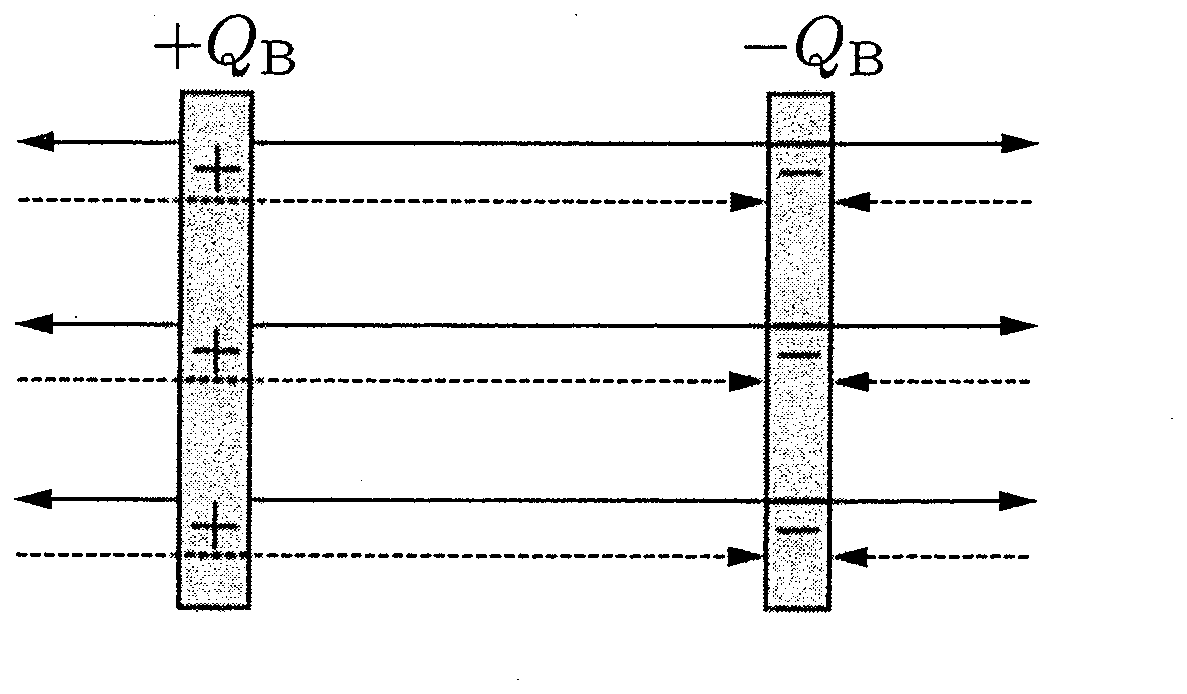
\includegraphics[keepaspectratio,width=66mm]{fig/n25_a57_zu1.png}\end{center}
       よって，極板間の部分は，$+Q_{\mathrm{B}}\U{C}$の電荷が作る右向き$2\pi kQ_{\mathrm{B}}$本の電気力線と，$-Q_{\mathrm{B}}\U{C}$の電荷が作る右向き$2\pi kQ_{\mathrm{B}}$本の電気力線との重なりになるので，その間での電場の強さは
       \[\frac{2\pi kQ_{\mathrm{B}}\times 2}{S}=\frac{4\pi k}{S}\cdot\frac{\varepsilon_{\mathrm{r}}\varepsilon_0SV}{d}\]
       であるが，ここでクーロンの法則の比例定数$k$と真空の誘電率$\varepsilon_0$との間には，
       \[k=\frac{1}{4\pi\varepsilon_0}\]
       の関係があるので，これを利用して整理すると，極板上の電荷$+Q_{\mathrm{B}}\U{C}$，$-Q_{\mathrm{B}}\U{C}$が極板間に作っている電場の強さは，
       \[\frac{4\pi k}{S}\cdot\frac{\varepsilon_{\mathrm{r}}\varepsilon_0SV}{d}=\frac{\varepsilon_{\mathrm{r}}V}{d}\U{V/m}\Ans\]
\ko{7} 誘電分極\Ans
\ko{8} 実際の極板間の電場は，(5)で求めた$E_{\mathrm{B}}=\dfrac{V}{d}\U{V/m}$であるから，誘電体の表面に発生する分極電荷によって，
       \[\frac{\varepsilon_{\mathrm{r}}V}{d}-E_{\mathrm{B}}=(\varepsilon_{\mathrm{r}}-1)\frac{V}{d}\U{V/m}\Ans\]
       だけ電場が弱められていることが分かる．
\ko{9} 誘電体表面に発生する分極電荷を$+q\U{C}$，$-q\U{C}$とおく．これらの分極電荷が誘電体の内部に作る電場の強さは，(6)と同様にガウスの法則を適用して考えればよい．
       \begin{center}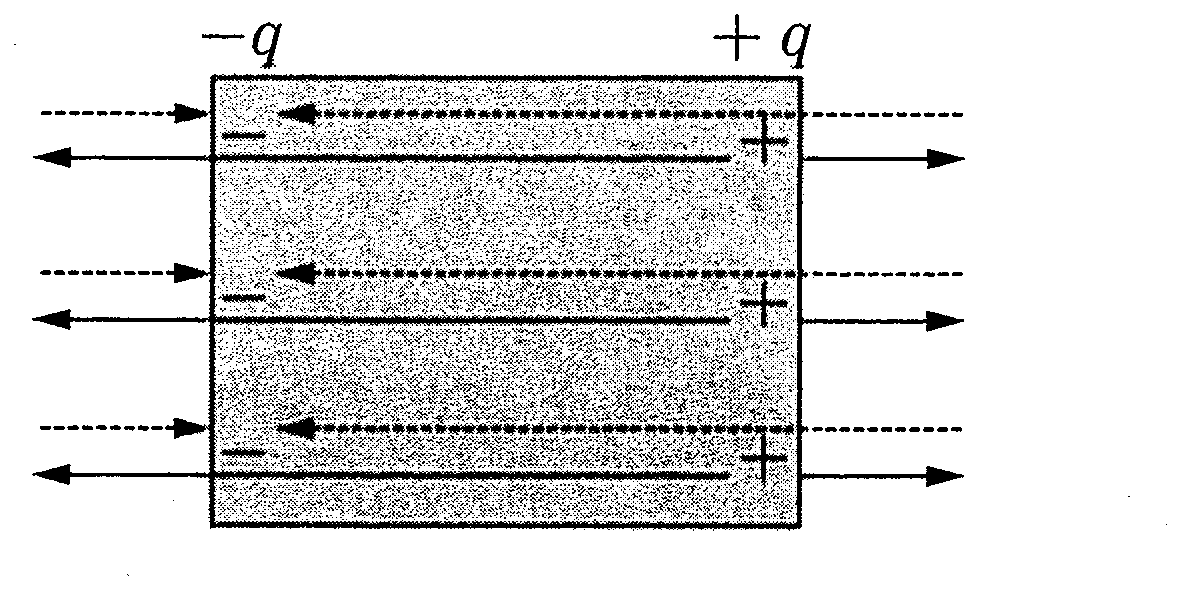
\includegraphics[keepaspectratio,width=64mm]{fig/n25_a57_zu2.png}\end{center}
       前図のように考えればこれらの電荷が誘電体内部に作る電場の強さが求められる．誘電体内部での電場は，$+q\U{C}$の電荷が作る左向き$2\pi kq$本の電気力線と，$-q\U{C}$の電荷が作る右向き$2\pi kq$本の電気力線との重なりになるので，その強さは
       \[\frac{2\pi kq\times 2}{S}=\frac{4\pi k}{S}q\U{V/m}\]
       であるが，(8)よりこの大きさが$(\varepsilon_{\mathrm{r}}-1)\dfrac{V}{d}\U{V/m}$であるから，
       \[\frac{4\pi k}{S}q=(\varepsilon_{\mathrm{r}}-1)\frac{V}{d}\]
       が成立する．これを解いて，
       \[\begin{aligned}
         q&=(\varepsilon_{\mathrm{r}}-1)\frac{V}{d}\cdot\frac{S}{4\pi k}\\
          &=(\varepsilon_{\mathrm{r}}-1)\frac{\varepsilon_0SV}{d}\U{C}\Ans
       \end{aligned}\]
\end{komon}

\MonN{58}{コンデンサーと静電エネルギー}\par\nopagebreak
\begin{sisin}
回路中に抵抗が含まれているが，定常状態の電荷が動いていない状態では回路中に電流が流れておらず，このような場合には抵抗には電圧がかからない．
\end{sisin}
\KaiHead
\begin{komon}
\ko{1} スイッチの操作前後の回路図は下の通りである．この際，スイッチ$\mathrm{S}_2$は開いたままであるから，点線で囲んだ二つの枠内について総電荷が保存される．次図のように文字を取る．
       \begin{center}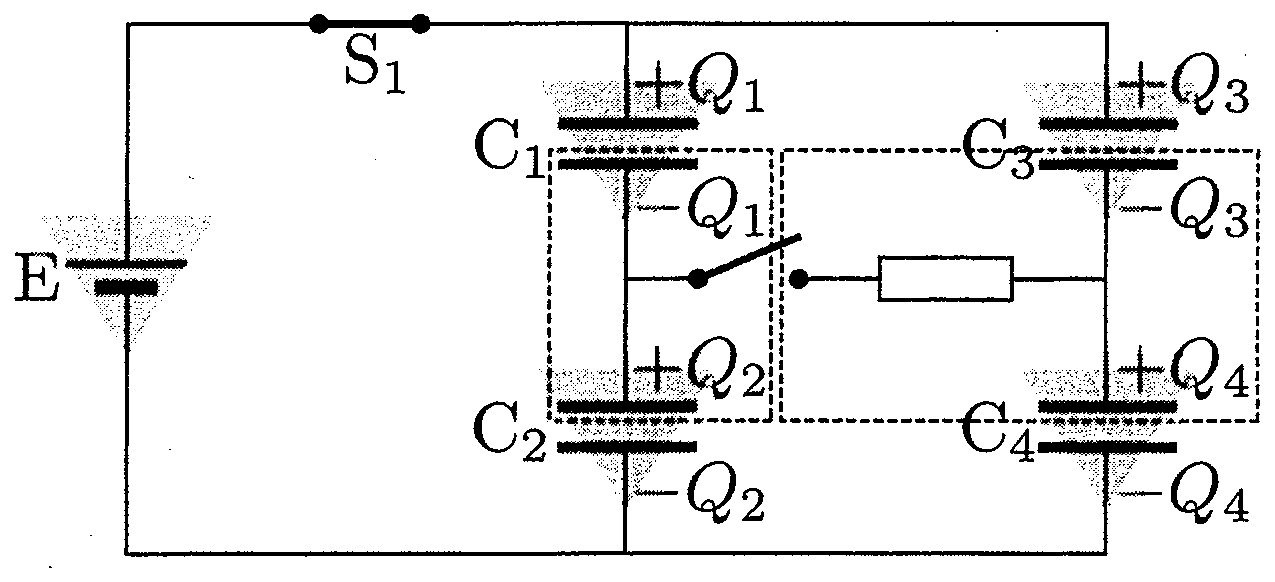
\includegraphics[keepaspectratio,width=66mm]{fig/n25_a58_zu1.png}\end{center}
       このとき，閉ループを作っているのは左側のループおよび外周部分の二つであり，これらに対してキルヒホッフの第二法則を用いると，
       \[10V=\frac{Q_1}{3C}+\frac{Q_2}{2C}\]
       \[10V=\frac{Q_3}{4C}+\frac{Q_4}{6C}\]
       また，点線枠内の総電荷が保存する．よって，
       \[0+0=-Q_1+Q_2,\quad 0+0=-Q_3+Q_4\]
       である．以上4式を整理すると，
       \[\begin{aligned}
         &Q_1=Q_2=12CV\U{C}\\
         &Q_3=Q_4=24CV\U{C}\Ans
       \end{aligned}\]
       \begin{chuu}
       上述の解答で，キルヒホッフの第二法則としては右側のループに対して
       \[0=-\frac{Q_1}{3C}-\frac{Q_2}{2C}+\frac{Q_3}{4C}+\frac{Q_4}{6C}\]
       という式を立てることも可能だが，敢えて外周のループを取った．このようにして式を立てておくと，変数$Q_1$，$Q_2$の組の式と$Q_3$，$Q_4$の組の式に分けられるため，その後の計算が簡単に済ませられるからである．このように，複数の回路にキルヒホッフの第二法則を用いることが可能な場合はどれを利用すると計算が楽になるかを考えよ．
       \end{chuu}
\ko{2} 各コンデンサーに蓄えられた静電エネルギーの和は，
       \[\begin{aligned}
         U&=\frac{Q_1^2}{2\cdot 3C}+\frac{Q_2^2}{2\cdot 2C}+\frac{Q_3^2}{2\cdot 4C}+\frac{Q_4^2}{2\cdot 6C}\\
          &=180CV^2\U{J}\Ans
       \end{aligned}\]
\ko{3} $\mathrm{S}_1$を開いても電荷は移動しない．この状態からスイッチ$\mathrm{S}_2$を閉じると，スイッチ$\mathrm{S}_2$の両側の電位が等しくなるようにコンデンサー極板上の電荷が移動する．各コンデンサーの上側極板に帯電する電気量をそれぞれ$Q_1^\prime$，$Q_2^\prime$，$Q_3^\prime$，$Q_4^\prime\U{C}$とおくと，帯電状態は次図のように変化する．
       \begin{center}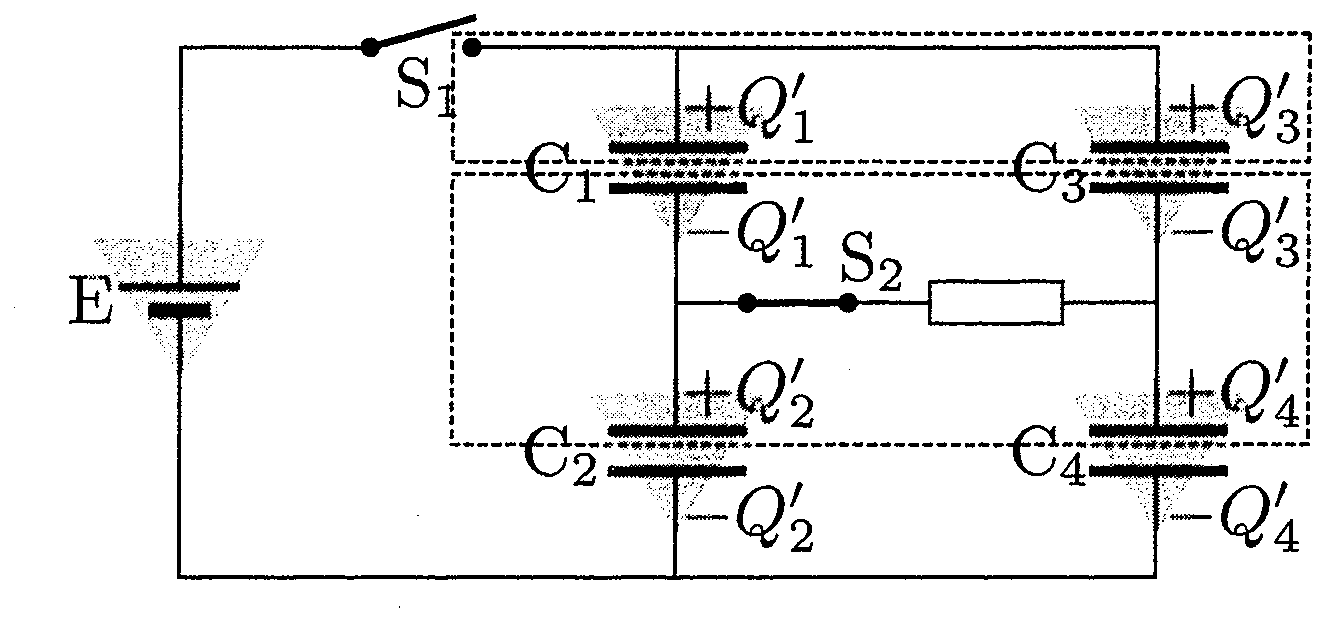
\includegraphics[keepaspectratio,width=68mm]{fig/n25_a58_zu2.png}\end{center}
       閉ループを作っているのは右上の部分および右下の部分の二つだけであるから，これらのループに対してキルヒホッフの第二法則を用いると，
       \[0=\frac{Q_1^\prime}{3C}-\frac{Q_3^\prime}{4C},\quad 0=\frac{Q_2^\prime}{2C}-\frac{Q_4^\prime}{6C}\]
       である．また，点線枠内に着目すると，ここはスイッチ操作前後について，回路の他の部分と接続していない．よって，この部分に対して電荷保存則を適用すると，
       \[+Q_1+Q_3=+Q_1^\prime+Q_3^\prime\]
       \[-Q_1+Q_2-Q_3+Q_4=-Q_1^\prime+Q_2^\prime-Q_3^\prime+Q_4^\prime\]
       である．以上4式を整理して計算して各電荷を求めると，
       \[Q_1^\prime=\frac{108}{7}CV\U{C},\quad Q_2^\prime=9CV\U{C}\]
       \[Q_3^\prime=\frac{144}{7}CV\U{C},\quad Q_4^\prime=27CV\U{C}\Ans\]
       \begin{bsHosoku}{参考}
       変数が多いので上述の4式の整理はうまく考えながら行うこと．まず，電荷保存の法則を先に利用すると，
       \[+Q_1^\prime+Q_3^\prime=36CV\]
       \[-Q_1^\prime+Q_2^\prime-Q_3^\prime+Q_4^\prime=0\]
       より，
       \[Q_2^\prime+Q_4^\prime=36CV\]
       これらとキルヒホッフの第二法則をそれぞれ組み合わせれば求められる．
       \end{bsHosoku}
\end{komon}

\MonN{59}{多極板コンデンサー}\par\nopagebreak
\begin{sisin}
多極板コンデンサーの問題は，間に導線を仮想するなどして複数のコンデンサーに分解し，前問までと同様な回路図に書き直せば，後は今までの問題と全く同じ攻め方で解ける（25.7）．

{\gtfamily 接地（アース）されている点は電位が$0$になると同時に，自由に電荷が出入りすることができる}（25.4）．

電気容量は極板間隔に\underline{反比例}するから，極板間隔が半分になれば電気容量は2倍になることに注意．
\end{sisin}
\KaiHead
\begin{komon}
\ko{1} 極板$\mathrm{AD}$および$\mathrm{DB}$からなるコンデンサーの極板間隔はともに$d\U{m}$なので，電気容量はいずれも
       \[\frac{1}{2}C\cdot\frac{2d}{d}=C\U{F}\]
       である．

       この多極板コンデンサーは次図のように書き換えることができるが，スイッチを閉じた後，$\mathrm{A}$，$\mathrm{B}$の電位は$0\U{V}$，$\mathrm{D}$の電位は$V\U{V}$であるから$\mathrm{D}$側の極板に正電荷が蓄えられる．これをそれぞれ$+q_1$，$+q_2\U{C}$とすると，$\mathrm{A}$，$\mathrm{B}$の$\mathrm{D}$側に蓄えられている電荷はそれぞれ$-q_1$，$-q_2\U{C}$である．
       \begin{center}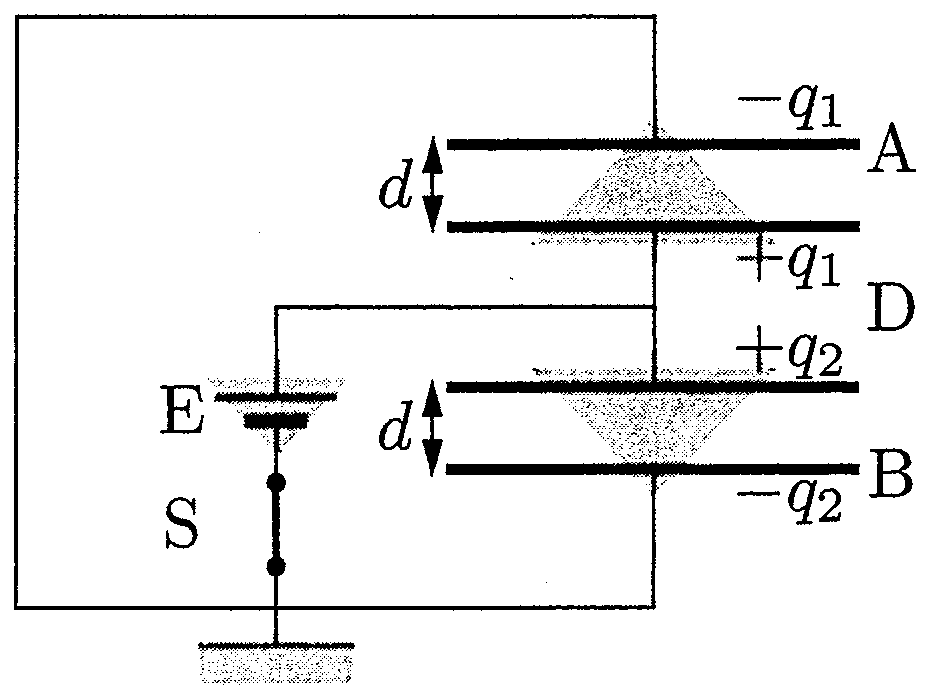
\includegraphics[keepaspectratio,width=58mm]{fig/n25_a59_zu1.png}\end{center}
       上側のループおよび下側のループに対してキルヒホッフの第二法則を用いると，
       \[V=\frac{q_1}{C},\quad V=\frac{q_2}{C}\]
       であるから，
       \[q_1=q_2=CV\U{C}\]
       である．

       今，金属板$\mathrm{D}$を二つに分解して考えているから，金属板$\mathrm{D}$に蓄えられている電気量は
       \[Q=+q_1+q_2=2CV\U{C}\Ans\]
\ko{2} 図の点線のように金属板$\mathrm{D}$を$\mathrm{A}$の方向に距離$x\U{m}$だけ移動したときには，$\mathrm{AD}$間および$\mathrm{DB}$間のコンデンサーの電気容量はそれぞれ，
       \[C_1=\frac{d}{d-x}C\U{F},\quad C_2=\frac{d}{d+x}C\U{F}\]
       である．スイッチ$\mathrm{S}$を開いてから，金属板$\mathrm{D}$を移動させて電気容量を変化させると電荷分布が変化する．極板$\mathrm{A}$，$\mathrm{B}$に蓄えられる電荷を$Q_1$，$Q_2\U{C}$として電荷分布を図示すると次図のように考えられる．
       \begin{center}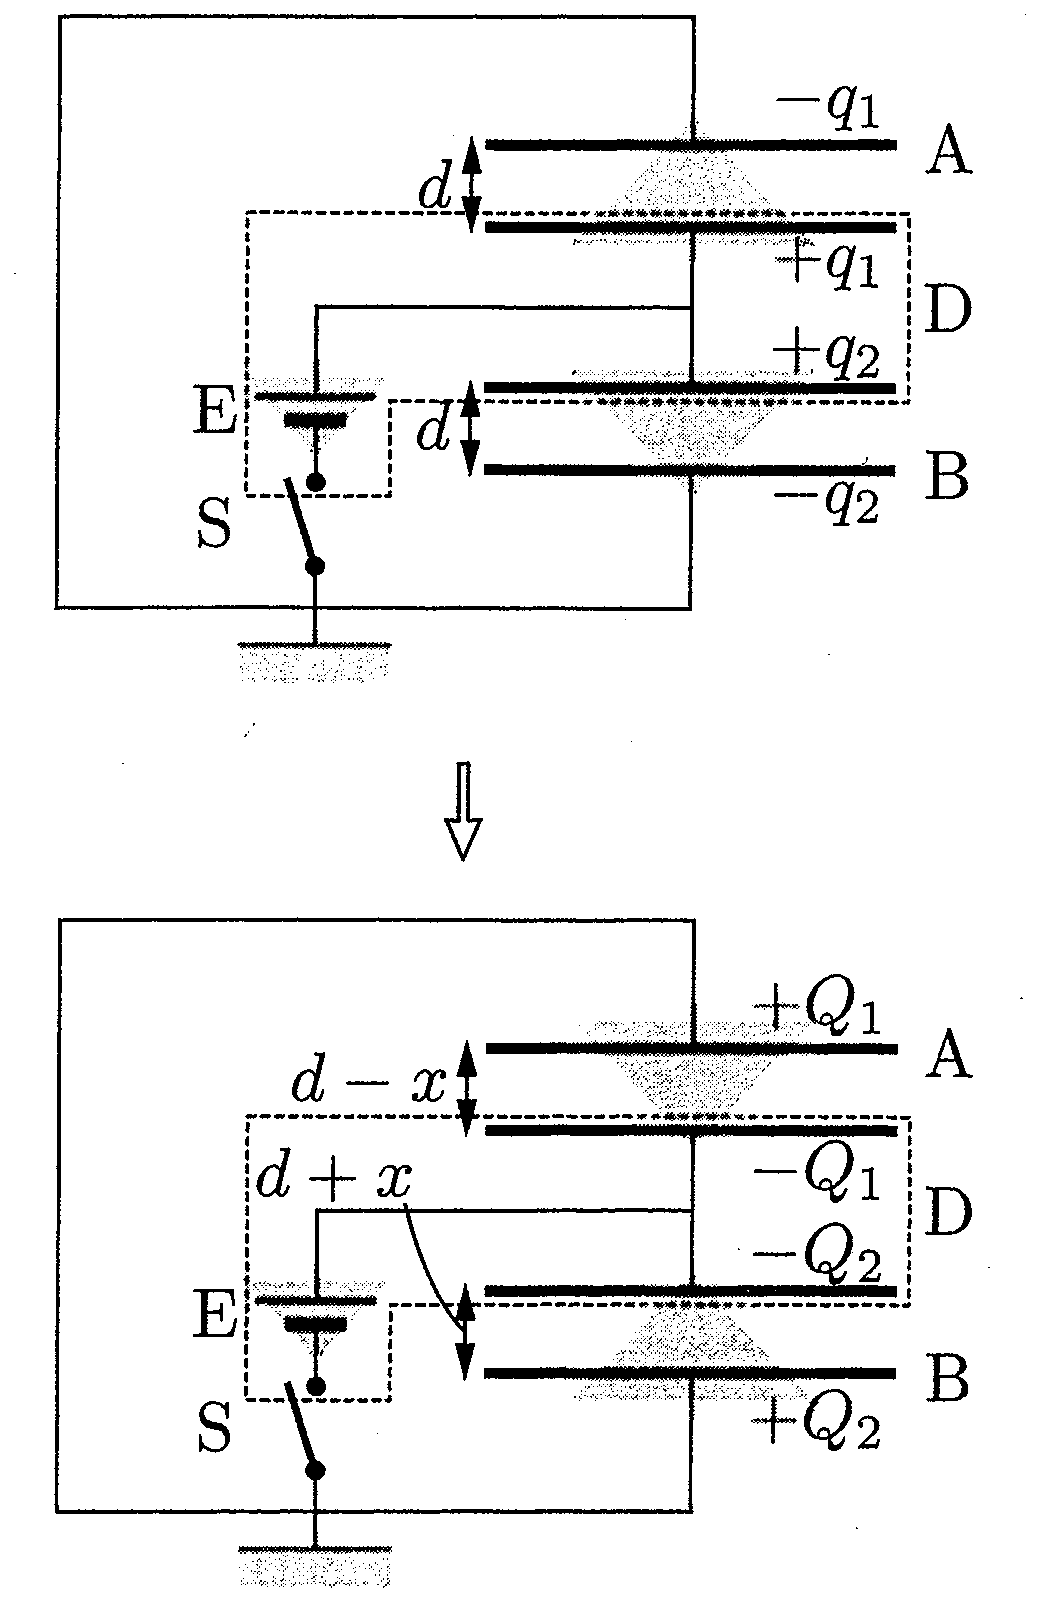
\includegraphics[keepaspectratio,width=60mm]{fig/n25_a59_zu2.png}\end{center}
       このとき，閉ループを作っているのは外周のループのみであり，これに対してキルヒホッフの第二法則を用いると，
       \[0=-\frac{Q_1}{C_1}+\frac{Q_2}{C_2}\]
       また，点線枠内の総電荷が保存する．よって，
       \[+q_1+q_2=-Q_1-Q_2\]
       である．以上2式を整理すると，
       \[\begin{aligned}
         &Q_1=-\frac{d+x}{d}CV\U{C}\\
         &Q_2=-\frac{d-x}{d}CV\U{C}\Ans
       \end{aligned}\]
       \begin{chuu}
       出てきた答えは負の値であるが，これは実際には$\mathrm{A}$，$\mathrm{B}$の極板上の電荷が負であり，$\mathrm{D}$側に正電荷が蓄えられていたことを示している．問題文で問われているのは極板$\mathrm{A}$，$\mathrm{B}$に蓄えられる電荷$Q_1$，$Q_2\U{C}$であるが，このような場合には$\mathrm{A}$，$\mathrm{B}$に\underline{正電荷}$Q_1$，$Q_2\U{C}$が蓄えられていると\underline{仮定}して式を立てておき，出てきた答えを，符号をつけたまま答えればよい．
       \end{chuu}
\end{komon}

\end{multicols}
